%/**
% * LaTeX thesis template (main file)
% * @author : Alexander willner <alex@willner.ws>
% * @url    : http://github.com/thesis
% */

% include config ---------------------------------------------------------------
\RequirePackage{pdf14}                 % PDF/A2-b compatibility
%\PassOptionsToPackage{demo}{graphicx} % for faster drafts
% document configuration -------------------------------------------------------
\documentclass[
        %pagesize,              % put paper size information into document
        a4paper,                % use a5paper for ISO A5; use a4paper for ISO A4
        pdftex,                 % PDF output
        %fontsize=12pt,         % font size
        headsepline,            % use headinclude also! (see M. Kohm)
        footsepline,            % use footinclude also! (see M. Kohm)
        headinclude,            % count head to text body (not to margin)
        footinclude,            % count foot to text body (not to margin)
        %BCOR8mm,               % set extra margin for book fixation
        headsepline,            % line on the top
        titlepage,              % show a title page
        %draft,                 % show under-/overfull boxes, hide images
        %demo=true,             % faster compile time
        %DIV=calc,              % calculate a nice type area
        %listof=totoc,          % List of Listings to ToC
        %oneside,               % e.g. same headings for odd and even pages
        %oneside=true,          % e.g. same headings for odd and even pages
        %twoside=false,         % e.g. same headings for odd and even pages
        %open=any,              % allows chapters to occur on left hand pages
        %openany,               % allows chapters to occur on left hand pages
        %ngerman,               % German language support
        %numbers=noendperiod    % no number at the end (German DUDEN)
%]{scrbook}
]{book}
% ------------------------------------------------------------------------------


% lang config ------------------------------------------------------------------
\usepackage[ngerman,english]{babel}          % German language support
%\usepackage{bibgerm}                        % German bibliography support
%\usepackage[babel,german=quotes]{csquotes}  % German language support
% ------------------------------------------------------------------------------


% basic packages ---------------------------------------------------------------
%\usepackage{tocloft}                         % Tweaks for large ToCs
%\cftsetpnumwidth{2em}                        % Tweaks for large ToCs
%\usepackage[demo]{graphicx}                  % faster compile time
% bugfixes ---------------------------------------------------------------------
%\let\spvec\vec                   % llncs with amsmath bugfix
%\let\vec\accentvec               % llncs with amsmath bugfix
%\newcommand{\subparagraph}{}     % IEEETrans with titlesec bugfix

%\makeatletter                    % for old listings package
%\@ifundefined{float@listhead}{}{%
%    \renewcommand*{\lstlistoflistings}{%
%        \begingroup
%            \if@twocolumn
%                \@restonecoltrue\onecolumn
%            \else
%                \@restonecolfalse
%            \fi
%            \float@listhead{\lstlistlistingname}%
%            \setlength{\parskip}{\z@}%
%            \setlength{\parindent}{\z@}%
%            \setlength{\parfillskip}{\z@ \@plus 1fil}%
%            \@starttoc{lol}%
%            \if@restonecol\twocolumn\fi
%        \endgroup
%    }%
%}
%\makeatother
% ------------------------------------------------------------------------------

% macro: ifpackageloaded -------------------------------------------------------
\makeatletter
\providecommand{\IfPackageLoaded}[2]{\@ifpackageloaded{#1}{#2}{}}
\providecommand{\IfPackageNotLoaded}[2]{\@ifpackageloaded{#1}{}{#2}}
\providecommand{\IfElsePackageLoaded}[3]{\@ifpackageloaded{#1}{#2}{#3}}
\makeatother
% ------------------------------------------------------------------------------

% File encoding: Normal UTF8 ---------------------------------------------------
\usepackage{cmap}                     % Support copy and search for pdflatex
%\input{glyphtounicode}                % Support copy and search for pdflatex
%\pdfgentounicode=1                    % Support copy and search for pdflatex
\IfPackageNotLoaded{CJKutf8}{\usepackage[utf8]{inputenc}}
\makeatletter
\def\UTFviii@defined#1{%
  \ifx#1\relax
      ((TODO:\@ Fix weird character here))%
  \else\expandafter
    #1%
  \fi
}
\makeatother
% ------------------------------------------------------------------------------

% ------------------------------------------------------------------------------
\usepackage{amssymb}                  % Springer Verlag (pdflatex)
\usepackage[hyphens]{url}             % Create URLs in the document
\usepackage[
spacing=true,                         % Fonts: spacing?
kerning=true,
tracking=true,                        % Fonts: hyphenatable letterspacing
expansion=true,                       % Fonts: better grey value
protrusion=true]{microtype}           % Fonts: margin kerning
\microtypecontext{spacing=nonfrench}
\usepackage[T1]{fontenc}              % Font encoding: T1
\usepackage{textcomp}                 % For the Euro sign
\usepackage{booktabs}                 % Nice tables
\usepackage{listings}                 % Nice listings
\usepackage{listingsutf8}             % Listings with UTF-8
\lstset{columns=fullflexible,         % Listings in multicolumn mode
        breaklines=true,              % Listings with long lines
        xleftmargin=3em,              % Correct indentation
        basicstyle=\scriptsize,       % Small text
        numbers=left,                 % Show numbers
        stepnumber=1,                 % For each line
        inputencoding=utf8            % Enable UTF8
        }
\usepackage{algorithmic}              % Nice pseudo code
\usepackage[table]{xcolor}                   % To use and define colors
\definecolor{LinkColor}{rgb}          % Link color
{0.31,0.46,.64}                       %
\definecolor{MarginColor}{rgb}        % Margin color
{0.31,0.46,.64}                       %
\usepackage{subcaption}               % Subfigures
\usepackage{wrapfig}                  % Use floating images
\usepackage{stfloats}                 % Makes LaTeX honour ‘[b]’ placement
\usepackage{amsmath}                  % For eqref
\usepackage{paralist}                 % For inline lists
%\usepackage{fixltx2e}                 % Provides fixes for LaTeX (not needed for anymore since 2015)
\usepackage{fix-cm}                   % Provides fixes for LaTeX
\usepackage{rotating}                 % e.g. for the special side margin notes
\usepackage{lipsum}                   % To add some dummy text
\usepackage{xspace}                   % Fixing some spacing issues
\usepackage{ellipsis}                 % Puts space around ellipses
%\usepackage{ragged2e}                 % New commands/env. for setting ragged text
%\usepackage{lmodern}                 % Nicer fonts (for all)
\usepackage{ltxtable}                 % Long complex tables
\usepackage{ltablex}                  % Long complex tables
\newcolumntype{L}{>{\raggedright\arraybackslash}X}
\usepackage[switch*,modulo]{lineno}   % Show line numbers
\usepackage{accsupp}                  % Don't copy line numbers (see below)
\renewcommand{\thelinenumber}{        % Line number printing mechanism
  \BeginAccSupp{ActualText={}}\arabic{linenumber}\EndAccSupp{}%
}
\usepackage{blindtext}                % insert blind texts
%\usepackage{cleveref}                 % To ref footnotes twice (use after hyperref)
%\crefformat{footnote}{#2\footnotemark[#1]#3}

\makeatletter
\newcommand*{\etc}{%
    \@ifnextchar{.}%
        {etc}%
        {etc.\@\xspace}%
}
\makeatother
\newcommand*{\eg}{e.g.\@\xspace}
\newcommand*{\ie}{i.e.\@\xspace}
\newcommand*{\cf}{cf.\@\xspace}

% To be used in the project specific config file:
%\usepackage[bf]{caption}[2008/08/24]  % Bold caption (better contrast)
%\usepackage{acronym}                  % For acronyms
%\usepackage[pdftex]{graphicx}         % Include images for pdflatex

\hyphenation{op-tical net-works semi-conduc-tor con-cept}

\renewcommand{\figurename}{Fig.}
\renewcommand{\tablename}{Tab.}
\newcommand{\sectionname}{Sec.}
\newcommand{\equationname}{Eq.}
\renewcommand{\lstlistlistingname}{List of Listings}

\makeindex

\setcounter{tocdepth}{3}
\newcommand{\mykeywords}[1]{\par\addvspace\baselineskip%
\keywordname\enspace\ignorespaces#1}
\makeatletter
\providecommand*{\toclevel@title}{99}
\providecommand*{\toclevel@author}{99}

\usepackage[tocindentauto]{tocstyle}      % fixing large roman page letters in ToC
\usetocstyle{standard}                    % same layout as before
\settocstylefeature{pagenumberbox}{\hbox} % fixing large roman page letters in ToC
% type setting ----------------------------------------------------------------
% no "Schusterjungen"
    \clubpenalty=10000
% no "Hurenkinder"
    \widowpenalty=10000
    \displaywidowpenalty=10000
% type setting ----------------------------------------------------------------

% annotations --------------------------------------------------------------
\newcommand{\annot}[2][]{%
    \pdfannot\ width \linewidth\ height 2\baselineskip\ depth 0pt{%
        /Subtype/Text%
        /Open false
        /Name /Comment%
        /CA .4%
        /C [.3 .6 .9]%
        /T (\pdfescapestring{#1})%            /Contents(\pdfescapestring{\detokenize{#2}})%
    }
}

\newcommand\aclc[1]{%
{%
\renewcommand{\url}[1]{}%
\renewcommand{\footnote}[1]{}%
\renewcommand{\cite}[1]{}%
\let\protect\relax%
\acl*{#1}%
}%
}
\newcommand\acfc[1]{%
{%
\renewcommand{\url}[1]{}%
\renewcommand{\footnote}[1]{}%
\renewcommand{\cite}[1]{}%
\let\protect\relax%
\acf*{#1}%
}%
}
\newcommand\todoremark[1]{%
	\color{blue}%
	((remark: #1))
	\color{black}%
}
\newcommand\todo[1]{%
	\color{red}%
	((todo: #1))
	\color{black}%
}
\newcommand\todotext[1]{%
    \todo{#1}%
	\color[gray]{0.8}%
	\blindtext[1]
	\color{black}%
}

\newcommand\todowrite[2]{%
  \color{red}%
  ((write about #1))
	\color[gray]{0.8}%
	Lorem ipsum dolor sit amet, consectetur adipisicing elit, sed do eiusmod tempor incididunt ut labore et dolore magna aliqua. Ut enim ad minim veniam, quis nostrud exercitation ullamco laboris nisi ut aliquip ex ea commodo consequat. Duis aute irure dolor in reprehenderit in voluptate velit esse cillum dolore eu fugiat nulla pariatur.
  #2
	\color{black}%
}


\newcommand\todosmall[1]{%
    \todo{#1}%
	\color[gray]{0.8}%
	Lorem ipsum dolor sit amet, consectetuer adipiscing elit. Etiam lobortis facilisis sem. Nullam nec mi et neque pharetra sollicitudin. Praesent imperdiet mi nec ante.
	\color{black}%
}
\newcommand\todoshort[1]{\todosmall{#1}}
\newcommand\todomid[1]{%
    \todo{#1}%
    \color[gray]{0.8}%
    Lorem ipsum dolor sit amet, consectetur adipisicing elit, sed do eiusmod tempor incididunt ut labore et dolore magna aliqua. Ut enim ad minim veniam, quis nostrud exercitation ullamco laboris nisi ut aliquip ex ea commodo consequat. Duis aute irure dolor in reprehenderit in voluptate velit esse cillum dolore eu fugiat nulla pariatur.
    \color{black}%
}

\usepackage{marginnote}               % Non floating margin notes
%for two-column layout
\makeatletter
\let\oldmarginnote\marginnote%
\renewcommand*{\marginnote}[1]{%
   \begingroup%
   \ifoddpage\value{page}
     \if@firstcolumn\reversemarginpar\fi
   \else
     \if@firstcolumn\else\reversemarginpar\fi
   \fi
   \needspace{\baselineskip}\oldmarginnote{#1}%
   \endgroup%
}
\makeatother
%\setlength{\marginparwidth}{0.7in}
\newcommand\sidenote[1]{\mbox{}%
  \marginnote{%
    \scriptsize%
    %\raggedright%
    \hspace{0pt}%
    \color{MarginColor}%
    %\begin{turn}{270}%
      \emph{#1}%
    %\end{turn}%
  }%
}%

% annotations --------------------------------------------------------------

% more listings ------------------------------------------------------------
\definecolor{grey}{rgb}{0.5,0.5,0.5}
\lstdefinelanguage{sparql}{
morecomment=[l][\color{black}]{\#},
morestring=[b][\color{black}]\",
morekeywords={SELECT,CONSTRUCT,DESCRIBE,ASK,WHERE,FROM,NAMED,PREFIX,BASE,OPTIONAL,FILTER,GRAPH,LIMIT,OFFSET,SERVICE,UNION,EXISTS,NOT,BINDINGS,MINUS,a},
sensitive=true
}
\lstdefinelanguage{ttl}{
sensitive=true,
morecomment=[l][\color{grey}]{@},
morecomment=[l][\color{black}]{\#},
morestring=[b][\color{black}]\",
}
\definecolor{groovyblue}{HTML}{0000A0}
\definecolor{groovygreen}{HTML}{008000}
\definecolor{darkgray}{rgb}{.4,.4,.4}

\lstdefinelanguage{Groovy}[]{Java}{
  keywordstyle=\color{groovyblue}\bfseries,
  stringstyle=\color{groovygreen}\ttfamily,
  keywords=[3]{each, findAll, groupBy, collect, inject, eachWithIndex},
  morekeywords={def, as, in, use},
  moredelim=[is][\textcolor{darkgray}]{\%\%}{\%\%}, % chktex 21
  moredelim=[il][\textcolor{darkgray}]{§§}
}
% more listings ------------------------------------------------------------

% IEEE copyright ---------------------------------------------------------------
\usepackage[pscoord]{eso-pic}
\newcommand{\ieeecopyright}[3]{
  \setbox0=\hbox{#3}
  \AddToShipoutPictureFG*{ \put(\LenToUnit{#1\paperwidth},\LenToUnit{#2\paperheight}){\vtop{{\null}\makebox[0pt][c]{#3}}}}
}
% IEEE copyright ---------------------------------------------------------------

% show the hex code of the unknown unicode character to actually find it ----
\usepackage{stringenc}
\usepackage{pdfescape}
\makeatletter
\renewcommand*{\UTFviii@defined}[1]{%
  \ifx#1\relax
    \begingroup
      % Remove prefix "\u8:"
      \def\x##1:{}%
      % Extract Unicode char from command name
      % (utf8.def does not support surrogates)
      \edef\x{\expandafter\x\string#1}% chktex 41
      \StringEncodingConvert\x\x{utf8}{utf16be}% convert to UTF-16BE
      % Hexadecimal representation
      \EdefEscapeHex\x\x
      % Enhanced error message
      \PackageError{inputenc}{Unicode\space char\space \string#1\space
                              (U+\x)\MessageBreak%
                              not\space set\space up\space
                              for\space use\space with\space LaTeX}\@eha%
    \endgroup
  \else\expandafter% chktex 41
    #1%
  \fi
}
\makeatother
% ---------------------------------------------------------------------------

% own requirement environment --------------------------------------------------
\makeatletter
\newcommand\requirement[3]{%
  \protected@write\@auxout{}{\string\CreateCounter{#1}}% chktex 21
  \crefname{my#1}{requirement}{requirements}\Crefname{my#1}{Requirement}{Requirements} %fixme:doesn't work
  \crefname{#1}{requirement}{requirements}\Crefname{#1}{Requirement}{Requirements} %fixme:doesn't work
  \@ifundefined{c@my#1}
    {#1??: #3}
    {\refstepcounter{my#1}\label{#2}#1\arabic{my#1}: #3}%
}
\newcommand{\CreateCounter}[1]{%
  \@ifundefined{c@my#1}
    {\newcounter{my#1}\global\@namedef{themy#1}{#1\arabic{my#1}}}% chktex 21
    {}%
}
\AtEndDocument{\let\CreateCounter\@gobble}% chktex 21
\makeatother
% ------------------------------------------------------------------------------
          % Default config
\usepackage[babel]{csquotes}                  % Biber wants it for babel
\usepackage[export]{adjustbox}                % For boxes around images
\usepackage{needspace}                        % used for embedding listings
%\usepackage{idxlayout}                       % fix index bugs and allow config
% ------------------------------------------------------------------------------

% basic config -----------------------------------------------------------------
\definecolor{LinkColor}{rgb}{0.0,0.2,0.5}     % Link color
\definecolor{MarginColor}{rgb}{0.0,0.2,0.5}   % Margin color
\definecolor{CaptionColor}{rgb}{0.0,0.2,0.5}  % Caption color
\definecolor{disabled}{gray}{0.5}             % Disabled text color
%\addtokomafont{sectioning}{\rmfamily}         % Serifs in headings
%\addtokomafont{sectioning}{\normalfont\scshape\rmfamily\color{CaptionColor}} % Serifs in headings
%\addtokomafont{sectioning}{\normalfont\rmfamily\color{CaptionColor}}        % Serifs in headings
\renewcommand{\lstlistlistingname}{List of Listings}
\renewcommand{\lstlistingname}{Listing}
\renewcommand{\contentsname}{Table of Contents}
\setcounter{secnumdepth}{4}
\setcounter{tocdepth}{2}
% basic config -----------------------------------------------------------------


% local config -----------------------------------------------------------------
\usepackage{pdflscape}
%\usepackage{subfig}
\usepackage{xmpincl}
%\includexmp{an-xmp-file-if-you-like}
\usepackage{enumitem}                   % More compact listings
\usepackage{float}                      % Provides the H float modifier option
% ------------------------------------------------------------------------------


% bibliography -----------------------------------------------------------------
\usepackage[
            style=numeric,%ieee,
            backref,
            backend=biber,
            defernumbers=true,
            useprefix=true,
            giveninits=true,
            %maxcitenames=2,
            maxbibnames=99, minbibnames=99,
            %doi=false,isbn=false,url=false,
            ]{biblatex}
\addbibresource{thesis_template.bib}
\defbibheading{empty}{}
\DeclareBibliographyCategory{cited}
\AtEveryCitekey{\addtocategory{cited}{\thefield{entrykey}}}
% ------------------------------------------------------------------------------


% acronyms ---------------------------------------------------------------------
\usepackage{acro}
\DeclareAcroPageStyle{dotfill}{inline}{
  punct = true,
  punct-symbol = \linebreak[1]\null\dotfill\nobreak%
}
\acsetup{
            single=false,
            sort=true,
            list-style=longtable,
            page-style=dotfill, % or =plain
            index, %  migh result in 'pdfTeX warning (dest): name... has been referenced but does not exist, replaced by a fixed one'
            pages=first,
            page-name={},
            pages-name={},
}
\robustify\footnote%
\robustify\url%
\newif\ifacrousefootnote%
\newcommand\acfootnote[1]{\ifacrousefootnote\footnote{#1}\fi}

\makeatletter\newif\ifnewacro%
\@ifpackagelater{acro}{2015/08/15}{% version 2.0 or later
\setboolean{newacro}{true}
}{% else hide footnotes and citations
\setboolean{newacro}{false}
\typeout{warning: your acro package is too old (<2.0)}
}%
\makeatother
\ifnewacro% show footnotes only once
    \ExplSyntaxOn%
    \NewAcroCommand\aclu%
      {
        \acro_is_used:nF {#1}
          { \acrousefootnotetrue\acro_cite: }
        \acro_long:n {#1}
      }
    \NewAcroCommand\Aclu%
      {
        \acro_if_acronym_used:nF {#1}
          { \acrousefootnotetrue\acro_cite: }
        \acro_first_upper:
        \acro_long:n {#1}
      }
    \ExplSyntaxOff%
\else
    \newcommand{\aclu}[1]{\acs{#1}}
    \newcommand{\Aclu}[1]{\Acs{#1}}
\fi
% ------------------------------------------------------------------------------


% chapter layout ---------------------------------------------------------------
%\usepackage[Sonny]{fncychap}                  % Nice chapter header
%\ChNameVar{\vspace*{-1in}\Large\rmfamily\vspace*{-2in}}   % Fancy chapter with serifs
%\ChTitleVar{\color{CaptionColor}\Large\rmfamily\scshape}  % Fancy chapter with serifs
\usepackage[clearempty]{titlesec}            % Suppress header and footer for empty pages
\setlength{\headheight}{1.1\baselineskip}
\titleformat{\chapter}[display]
  {\scshape\huge\color{CaptionColor}}
  {\filleft\Large\chaptertitlename~\thechapter}
  {2.5ex}
  {\titlerule\vspace{1ex}\filleft}
  [\vspace{1ex}\titlerule]
% ------------------------------------------------------------------------------


% more config ------------------------------------------------------------------
% todo: move to 'basic config'
\usepackage{lmodern}                          % Nicer fonts (for all) - times
\usepackage{mathptmx}                         % Nicer fonts (for all) - times
%\usepackage{scrhack}                         % Fix some scrbook issues
\usepackage{chapterthumb}                     % Fancy thumb index
\usepackage[chapter]{algorithm}               % Nice pseudo code
\usepackage{lettrine}                         % Drop characters, if you like
\renewcommand{\LettrineFontHook}{\color{CaptionColor}}
\usepackage[nohints]{minitoc}                 % ToC for chapters
\dominitoc[n]                                 % ToC: no caption
\renewcommand{\mtcSfont}{\small}              % ToC: small
\usepackage{makeidx}                          % Make an index
\makeindex                                    % Make an index
% ------------------------------------------------------------------------------


% spqueezing -------------------------------------------------------------------
%\usepackage{etoolbox}
%\makeatletter
%\patchcmd{\AC@@acro}
%  {\dotfill\pageref{acro:#1}}
%  {\nobreak\leaders\hbox{$\mkern -7mu \mkern \@dotsep mu\hbox{.}\mkern \@dotsep mu \mkern 7mu$}%
%   \hfill\nobreak\makebox[1.3em][r]{\pageref{acro:#1}}}
%  {}
%  {}
%\makeatother
% ------------------------------------------------------------------------------


% wall papger / logo on first page ---------------------------------------------
 \usepackage{wallpaper}
 \newlength\cornerXoffset%
 \newlength\cornerYoffset%
 \setlength\cornerXoffset{2cm}        % X
 \setlength\cornerYoffset{2cm}        % Y
 \newcommand\ThisLROffsetCornerWallPaper[2]{%
  \AddToShipoutPicture*{%
    \AtPageLowerLeft{%
      \parbox[b]{\paperwidth-\cornerXoffset}{%
        \hfill \includegraphics[width=#1\paperwidth,height=#1\paperheight,%
        keepaspectratio]{#2}%
        \vspace{\cornerYoffset}\null%
      }
    }
  }
 }
% ------------------------------------------------------------------------------


% page layout ------------------------------------------------------------------
\usepackage[pass,a4paper]{geometry}
%\usepackage[marginparwidth=.7in, marginparsep=0.2in]{geometry}
%\geometry{a4paper, bottom=4cm}
% \renewcommand{\topfraction}{0.9}
% \renewcommand{\bottomfraction}{0.9}
% \renewcommand{\textfraction}{0.07}         % allow minimal text w. figs
% \renewcommand{\floatpagefraction}{0.7}     % require fuller float pages
% \renewcommand{\dblfloatpagefraction}{0.7}  % require fuller float pages
% \renewcommand{\dbltopfraction}{0.9}        % fit big float above 2-col. text
% \renewcommand{\textfloatsep}{5mm}
% \setcounter{topnumber}{2}
% \setcounter{bottomnumber}{2}
% \setcounter{totalnumber}{4}                % 2 may work better
% \setcounter{dbltopnumber}{2}               % for 2-column pages
% ------------------------------------------------------------------------------


% hyperlinks (almost last package) ---------------------------------------------
\usepackage{hyperxmp}                 % Semantic meta data (RDF/XMP)
%\pdfminorversion=4                   % PDF/A compatbility
%\pdfobjcompresslevel=0               % PDF/A compatbility
%\pdfcompresslevel=0                  % PDF/A compatbility
\usepackage[pdftex,                   % Hyperlinks in PDFs
pdfa=true,                            % PDF/A compatbility (fix hyperlink with ghostscript)
unicode=true,                         % PDF/A compatbility
raiselinks=true,			                % calculate real height of the link
breaklinks,                           % break links
%backref=page,                        % backlinks in bibliography (section, slide, page, none)
%pagebackref=true,                    % backlinks in bibliography
hyperindex=true,                      % backlinkex index
linktocpage=true,                     % ToC links pages
bookmarks=true,                       % Bookmarks for PDF viewers
bookmarksopen=true,                   % Open bookmarks
bookmarksopenlevel=2,                 % How many levels to open
bookmarksnumbered=true,               % Numbers in the bookmarks
bookmarkstype=toc,                    % Type of bookmark
plainpages=false,                     % Anchors even on plain pages?
pageanchor=true,                      % Pages are linkable
pdfstartview=FitH,                    % Open document with Fit Width
pdfpagelabels=true,                   % set PDF page labels
pdfpagemode=UseOutlines,              % Show bookmarks in viewer
colorlinks,                           % Show colored links
linkcolor=LinkColor,                  % Link color
urlcolor=LinkColor,                   % URL color
anchorcolor=LinkColor,                % Anchor color
citecolor=LinkColor,                  % Cite color
menucolor=LinkColor,                  % Menu color
hypertexnames=true                    % Whatever ;)
]{hyperref}                           % Use hyperlinks
%\renewcommand*{\backref}[1]{[cited at page #1]} % Show formatted backlinks
\usepackage{bookmark}                 % Manually add PDF bookmarks
% ------------------------------------------------------------------------------


% cleveref with fixes ----------------------------------------------------------
\usepackage{cleveref}                 % To ref footnotes twice (use after hyperref)
\crefformat{footnote}{#2\footnotemark[#1]#3}
% ------------------------------------------------------------------------------


% glossary (last package) ----------------------------------------------------
\usepackage[xindy,nonumberlist,toc]{glossaries}
\newglossaryentry{Term}
{
  name=Term,
  description={A general-purpose term}
}
\newglossaryentry{Foo}
{
    name={Foo},
    description={Bar}
}

\setglossarystyle{altlist}
\renewcommand*{\glsgroupskip}{}
\makeglossaries%
% ------------------------------------------------------------------------------


% meta data --------------------------------------------------------------------
% meta data --------------------------------------------------------------------
\newcommand{\metaType}{PhD of templates}
\newcommand{\metaTypeShort}{Dr.-Tmpl.}
\newcommand{\metaWhy}{To get the degree in}
\newcommand{\metaHowFinal}{Submitted}
\newcommand{\metaHowNonFinal}{Draft}
\newcommand{\metaBoard}{Board}
\newcommand{\metaSubmitted}{Presented by}
\newcommand{\metaDate}{11.~Februar~2016}
\newcommand{\metaDateEn}{11.~February~2016}
\newcommand{\metaDateExam}{\metaDate}
\newcommand{\metaNumber}{2016--02}
\newcommand{\metaTitleLayouted}{Sophisticated Template\\for a Thesis}
\newcommand{\metaTitle}{Sophisticated Template for a Thesis}
\newcommand{\metaTitleShort}{Thesis Template}
\newcommand{\metaDegree}{MTA}
\newcommand{\metaBirthplace}{Born in Foo Bar}
\newcommand{\metaAuthor}{First Last}
\newcommand{\metaAuthorMail}{first.last@example.org}
\newcommand{\metaKeywords}{Foo, Bar, First, Last}
\newcommand{\metaSubject}{Template Subject}
\newcommand{\metaUniversity}{Template University}
\newcommand{\metaFaculty}{Template Faculty}
\newcommand{\metaDepartment}{Template Department}
\newcommand{\metaCitycode}{12345}
\newcommand{\metaCity}{City}
\newcommand{\metaCountry}{Country}
\newcommand{\metaURL}{http://example.org}
\newcommand{\metaChair}{Chair}
\newcommand{\metaChairName}{Prof.\ Dr.-Ing.\ Goo Gl}
\newcommand{\metaChairUniversity}{Industry}
\newcommand{\metaReviewer}{Reviewer}
\newcommand{\metaFirstReviewerName}{Prof.\ Dr.-Ing.\ Foo Bar}
\newcommand{\metaFirstReviewerUniversity}{Example University}
\newcommand{\metaSecondReviewerName}{Prof.\ Dr.\ Bar Foo}
\newcommand{\metaSecondReviewerUniversity}{Another University}
\newcommand{\metaThirdReviewerName}{Dr.\ John Smith}
\newcommand{\metaThirdReviewerUniversity}{My University}
\newcommand{\metaFourthReviewerName}{{\color{gray}Dr.\ Jon Doe}}
\newcommand{\metaFourthReviewerUniversity}{{\color{gray}BAR}}


\newcommand{\metaAuthorShort}{\metaAuthor}
\newcommand{\metaConference}{Conference}
\newcommand{\metaConferenceArea}{Area}
\newcommand{\metaDedication}{\scriptsize{Dedicated to my beloved family.}}
% ------------------------------------------------------------------------------

%%% Only for koma script
%\subject{\metaSubject}
%\title{\metaTitle}
%\author{\metaAuthor}
%\date{\metaDate}
%\dedication{\metaDedication}

\hypersetup{
      pdfauthor={\metaAuthorShort~<\metaAuthorMail>},
      pdfsubject={\metaSubject},
      pdftitle={\metaTitle},
      pdfkeywords={\metaKeywords},
      pdfcreator={http://github.com/thesis},
      pdfproducer={pdfTeX},
}

% ------------------------------------------------------------------------------


% final fixes ------------------------------------------------------------------
\righthyphenmin=2
\tolerance=2000
\emergencystretch=10pt
% ------------------------------------------------------------------------------

% PDF/A color profile ----------------------------------------------------------
\immediate\pdfobj stream attr{/N 3}  file{lib/resources/pdfa/srgb.icc}% chktex 1
\pdfcatalog{%
/OutputIntents [ <<
/Type /OutputIntent
/S/GTS_PDFA1
/DestOutputProfile \the\pdflastobj\space 0 R
/OutputConditionIdentifier (sRGB IEC61966-2.1)% chktex 8
/Info(sRGB IEC61966-2.1)% chktex 8 chktex 36
>> ]
}
% ------------------------------------------------------------------------------
     % inlcude general configuration
%\DeclareAcronym{PLC}{short={PLC}, long={Programmable Logic Controller}}
%\DeclareAcronym{Swoogle}{short={Swoogle}, long={}, cite={ding2004swoogle}, long-post={\acfootnote{\url{http://swoogle.umbc.edu}}}}
%\DeclareAcronym{}{short={}, long={}, short-indefinite={an},  long-indefinite={an}, cite={}, long-post={\acfootnote{\url{}}}, class=exclude}
%\DeclareAcronym{}{short={}, long={}}
\DeclareAcronym{ABAC}{short={ABAC}, long={Attributed Based Access Control}, cite={li2002design,Yuan2005}}
\DeclareAcronym{DBpedia}{short={DBpedia}, long={DBpedia}, cite={Auer2007}, long-post={\acfootnote{\url{http://dbpedia.org}}}, class=exclude}
       % inlcude acronyms
\DeclareUnicodeCharacter{0301}{}       % fixing an UTF-8 encoding issue
%\usepackage[norefs,nocites]{refcheck} % useful, but not working with cref
%\usepackage[doublespacing]{setspace}  % useful for reviewing a printout
%\PassOptionsToPackage{cmyk}{xcolor}   % PDF/A compatibility, skipped
%\usepackage[a-2b]{pdfx}               % PDF/A compatibility, skipped
\usepackage{pdflscape}

\newcommand{\isFinal}{true}            % Modify e.g. the title page
% ------------------------------------------------------------------------------


% include only required files for faster building ------------------------------
%\includeonly{src/03_requirements,src/06_implementation}
% ------------------------------------------------------------------------------


% begin thesis -----------------------------------------------------------------
\begin{document}
    \frontmatter
    \pagestyle{empty}
    \pagenumbering{alph}
    \pdfbookmark{Title}{title}
\begin{titlepage}
\newgeometry{left=35mm, right=35mm, top=35mm, bottom=35mm}


\begin{center}
\vspace*{2cm}
\LARGE{\metaTitleLayouted}\\
\normalsize

\vspace*{2cm}
\metaSubmitted%
\\
\metaAuthor, \metaDegree~\\
\metaBirthplace%
\\

\vspace*{2cm}
\metaFaculty%
\\
\metaUniversity%
\\
\metaWhy%
\\
\vspace*{0,5cm}
\metaType%
\\
-~{\metaTypeShort}~-% chktex: 8
\\
\vspace*{0,5cm}

\ifthenelse{\equal{\isFinal}{true}}{
\metaHowFinal%
}{
\metaHowNonFinal%
}
\end{center}

\ifthenelse{\equal{\isFinal}{true}}{

\vspace*{2cm}
\metaBoard:\\
\vspace*{.3cm}\\
\begin{tabular}{@{\hspace{1.5em}}ll}
\metaChair: & \metaChairName~(\metaChairUniversity) \\
\metaReviewer: & \metaFirstReviewerName~(\metaFirstReviewerUniversity) \\
\metaReviewer: & \metaSecondReviewerName~(\metaSecondReviewerUniversity)\\
\metaReviewer: & \metaThirdReviewerName~(\metaThirdReviewerUniversity)\\
\end{tabular}

\vspace*{1,9cm}
\metaDateExam%
\vspace*{0,9cm}

}{
\vspace*{6cm}
}

\begin{center}
\metaNumber\newline
\end{center}


\ThisLROffsetCornerWallPaper{.2}{resources/images/logo}   % logo in the corner

\restoregeometry%
\end{titlepage}

    \cleardoublepage\vspace*{100mm}
\begin{minipage}{109.5mm}
\section*{Affidavit}
I hereby declare that the following thesis ``\metaTitle'' has been
written only by the undersigned and without any assistance from third
parties.\\

Furthermore, I confirm that no sources have been used in the preparation
of this thesis other than those indicated in the thesis itself.\\[2cm]
\metaCity,
\metaDate%
\end{minipage}

    \cleardoublepage\pdfbookmark{Dedication}{dedication}
\begin{center}
\LARGE{\metaDedication}
\end{center}

    \cleardoublepage

    \pagestyle{scrheadings}
    \lohead[]{}
    \pagenumbering{roman}
    \setcounter{page}{1}
    \pdfbookmark{Acknowledgments}{acknowledgments}
\chapter*{Acknowledgments}

\todomid{thank your supervisors}

\todomid{thank your colleagues}

\todomid{thank your family and friends}

\vspace{0.5in}
\begin{flushright}
  \metaCity, February 12, 2016%\today%
\end{flushright}
\cleardoublepage{}
    \pdfbookmark{Abstract}{abstract}
\chapter*{Abstract}

{\setlength{\parindent}{-.1cm}%
\sidenote{Research Area:\\Foo Bar}%
\todomid{write about the research area}

\sidenote{Application Area:\\Bar Foo}
\todomid{write about the application area}

\sidenote{Research Issue:\\Foo Fooli}
\todomid{write about the research issue}

\sidenote{Own Approach:\\Bar Barli}
\todomid{write about the own approach}

\sidenote{Scientific Contributions}
\todomid{write about the scientific contributions}

\sidenote{Validation \& Outlook}
\todomid{write about the validation and outlook}

\cleardoublepage
\begin{otherlanguage}{ngerman}
\pdfbookmark{Zusammenfassung}{Zusammenfassung}
\chapter*{Zusammenfassung}%

\sidenote{For\-schungs\-be\-reich:\\Foo Bar}%
\todomid{write}

\sidenote{Ein\-grenz\-ung:\\Bar Foo}
\todomid{write}

\sidenote{Pro\-blem\-stel\-lung:\\Foo Fooli}
\todomid{write}

\sidenote{Eigener Ansatz:\\Bar Barli}
\todomid{write}

\sidenote{Wis\-sen\-schaft\-lich\-er Bei\-trag}
\todomid{write}

\sidenote{Va\-li\-die\-rung \& Aus\-blick}
\todomid{write}

\end{otherlanguage}

}
\cleardoublepage
\cleardoublepage

    \phantomsection
    % Change the depth for review
\pdfbookmark{Table of Contents}{toc}
\renewcommand{\contentsname}{Table of Contents}
\tableofcontents

\cleardoublepage
\phantomsection\addstarredchapter{\listfigurename}
\listoffigures

\cleardoublepage
\phantomsection\addstarredchapter{\lstlistlistingname}
\lstlistoflistings

\cleardoublepage
\phantomsection\addstarredchapter{\listtablename}
\listoftables

\cleardoublepage
\cleardoublepage

    \mainmatter
    \lohead[\putchapterthumb]{\putchapterthumb}
    \pagenumbering{arabic}
    \setcounter{page}{1}
    \linenumbers
    \acresetall%
    \cleardoublepage\chapter{Introduction}
\minitoc\label{sec:introduction}\vspace{.5cm}

\section{Background and Motivation}

\sidenote{Research Context: Foo}
\todomid{write about the research context \gls{Foo}}\index{Foo}

\sidenote{Research Area: Bar}
\todomid{write about the research area and \Cref{fig:intro:a}}\index{Bar}

\begin{figure}[H]
    \centering
    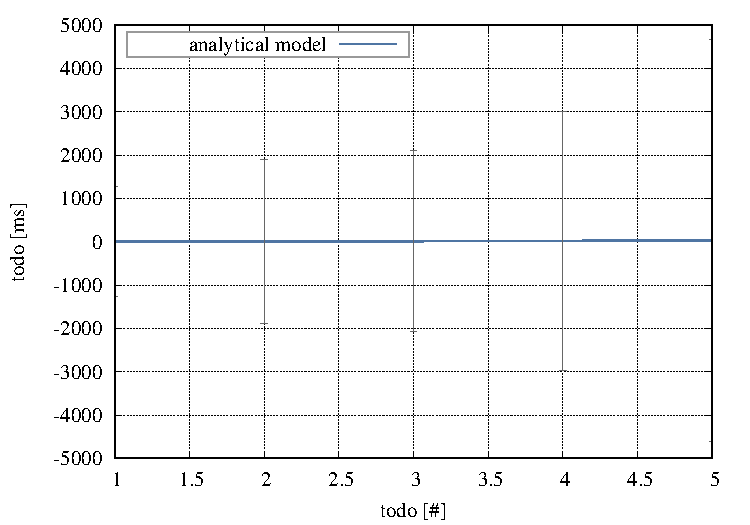
\includegraphics[width=.55\textwidth]{resources/images/example1}
    \caption{Example (based on~\cite{li2002design})}\label{fig:intro:a}
\end{figure}

\sidenote{Application Area: Foo Fooli}\index{Foo!Fooli}
\todomid{write about the application area~\cite{Heflin2004}}

\begin{figure}[H]
      \centering
      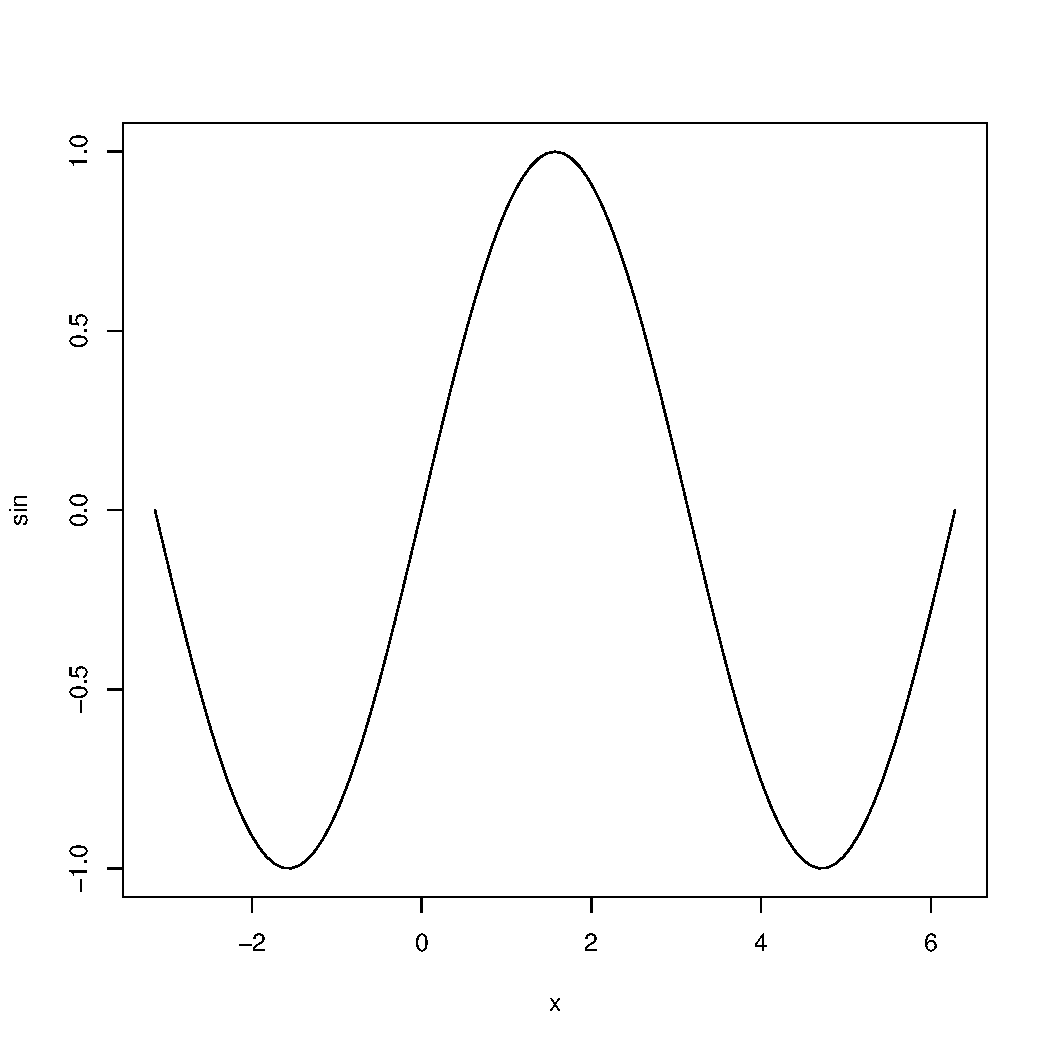
\includegraphics[width=.45\textwidth]{resources/images/example2}
      \caption{Another example~\cite{li2002design}}\label{fig:intro:b}
\end{figure}

\sidenote{Research Focus: Bar Barli}\index{Bar!Barli}
\todomid{write about the research focus and \Cref{fig:intro:b}}

\sidenote{Taxonomy}\index{Taxonomy}
\todomid{write about the taxonomy and \ac{ABAC}}

\begin{figure}[htbp]
      \centering
      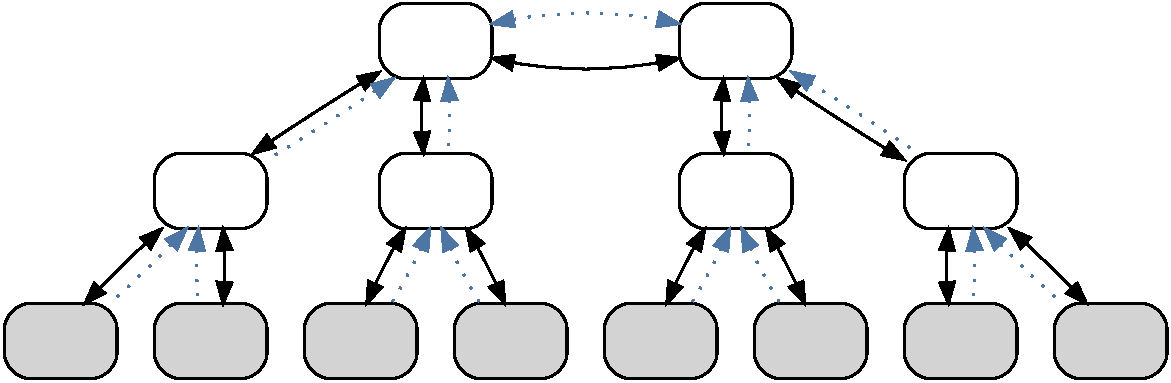
\includegraphics[width=.75\textwidth]{resources/images/example3}
      \caption{Taxonomy}
\end{figure}

\section{Problem Statement}\index{Requirements}
%2.11.4.1 IoT interoperability necessary framework
\sidenote{State of the Art}
\todomid{write about the State of the Art}

\sidenote{Issue:\\Example 1}
\todomid{write about the first issue}

\sidenote{Issue:\\Example 2}
\todomid{write about the second issue}

\sidenote{Synopsis}
\todomid{write about the synopsis of the issues and \Cref{fig:intro:c}}

\begin{figure}[htbp]
    \centering
    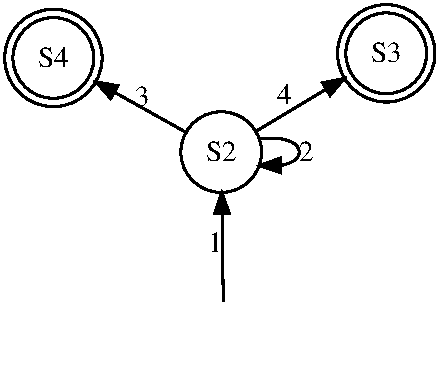
\includegraphics[width=.5\textwidth]{resources/images/job_lifecycle}
    \caption{Relationship between issues}\label{fig:intro:c}
\end{figure}

\section{Assumptions and Scope}

\sidenote{Research Assumptions}
\todomid{write about the research assumptions~\cite{li2002design}}

\sidenote{Research Scope}
\todomid{write about the research scope --- \Cref{fig:intro:a,fig:intro:b,fig:intro:c}}


\section{Objectives and Contributions}

\begin{figure}[htbp]
    \centering
    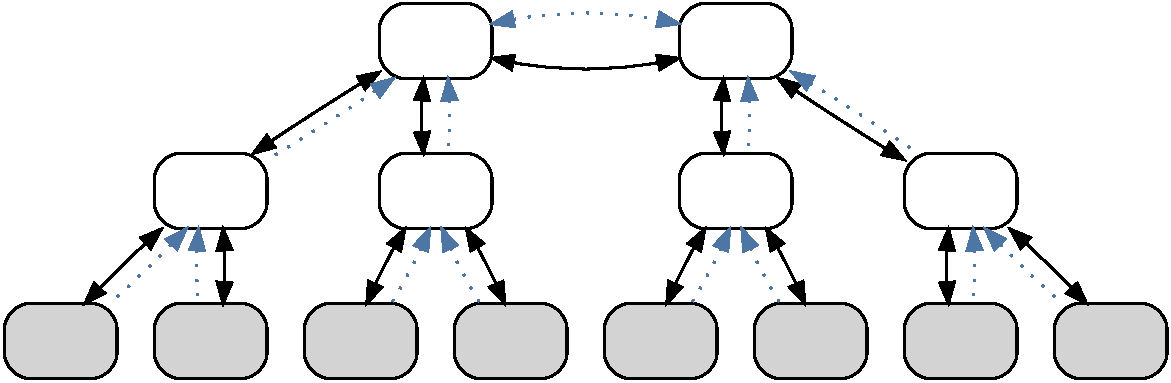
\includegraphics[width=.55\textwidth]{resources/images/example3}
    \caption{Structure of research}\label{fig:intro:struct}
\end{figure}

\sidenote{Research Objectives \& Contributions}
\todomid{write about the research objectives and \aclu{DBpedia} and \Cref{fig:intro:struct}}

\section{Methodology and Outline}

\todomid{write about the research outline and \Cref{fig:intro:methodology}. Summarize \Cref{sec:introduction,sec:sota,sec:reqs,sec:contrib1,sec:contrib2,sec:contrib3,sec:eval,sec:summary}.}

\begin{sidewaysfigure}
    \centering
    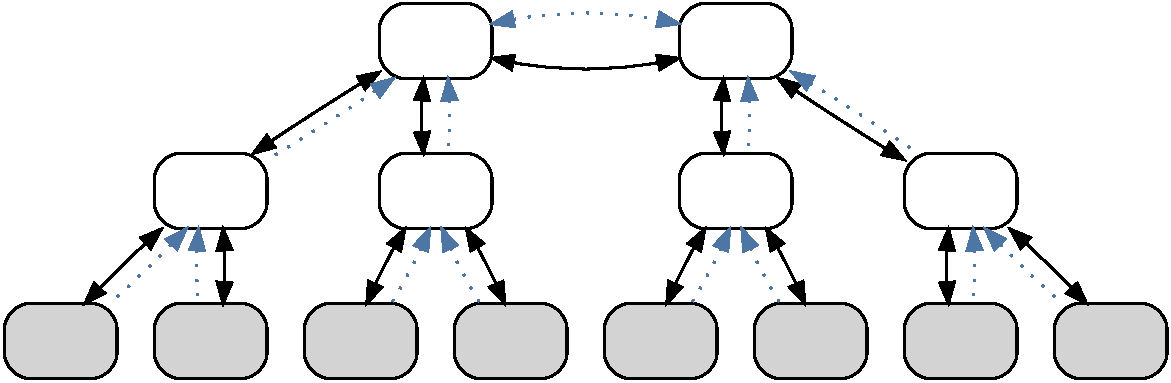
\includegraphics[width=.7\textwidth]{resources/images/example3}
    \caption{Workflow of the research and structure of the thesis}\label{fig:intro:methodology}
\end{sidewaysfigure}

    \cleardoublepage
\setlist[enumerate,1]{%
  label=\arabic*.,
}

\newlist{inlinelist}{enumerate*}{1}
\setlist*[inlinelist,1]{%
  label=(\roman*),
}



\chapter{State of the Art}\label{sec:sota}\minitoc\vspace{.5cm}
\index{SotA}

\section{Introduction}
This chapter provides an understanding of the relevant terms, technologies, and standards in the field of Internet of things and Semantic interoperability. It starts with an introduction to the Internet of things with specifying its visions and the standardization efforts in this research area. Afterward, the most relevant standardization work of the IoT is presented. Eventually, after introducing the semantic web and semantic technology, the Semantic Web stack for the IoT is discussed, and the appropriate ontologies created for IoT are given. Finally, the openMTC platform is introduced as well as its architecture and most relevant features.

\section{Internet of Things}\index{Related Area}

In 1998, Kevin Ashton introduced the paradigm "Internet of things" (IoT)~\cite{bookiot}. Since then, this novel paradigm has attracted massive attention in academia as well as in industry~\cite{hindi}. \par
The IoT is intended to add a new dimension to the world of information and communication by defining a network in which physical devices have their virtual representation on the Internet, thus enabling the exchange of data between physical things, applications, and people. This interconnection allows the intercommunication and handling of things by other things or by humans, leading to the automation of different tasks and scenarios~\cite{gazi}. A thing can refer to wide variety of physical objects, from a humidity sensor at a farm to a heart rate monitoring device or a motor in a space station. It can refer virtually to a mobile phone application or enterprise resource planning software running in the cloud. This new dimension in the communications world is illustrated in the following: figure~\ref{fig:contrib2:d}

\begin{figure}[htbp]
    \centering
    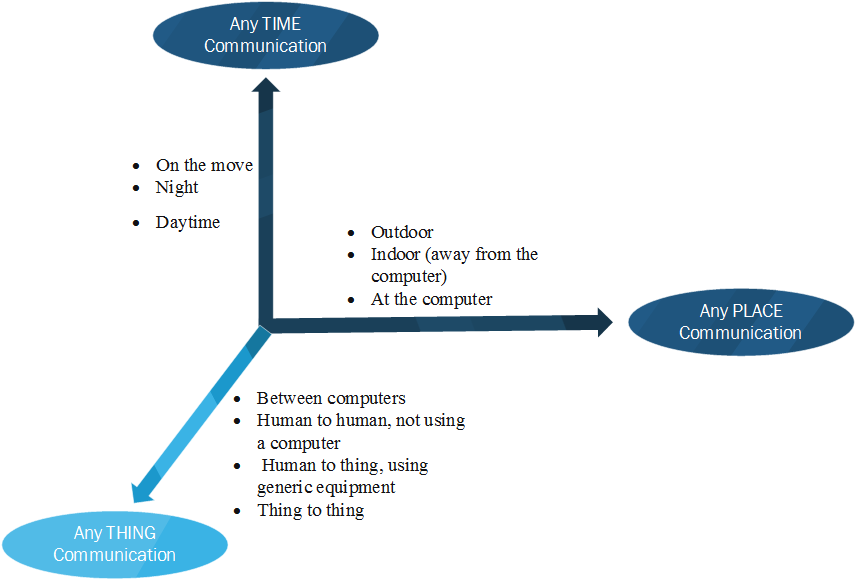
\includegraphics[width=1\textwidth]{resources/images/dimonsion}
    \caption{The new dimension introduced in the Internet of things adapted from~\cite{gazi} }\label{fig:contrib2:d}
\end{figure}
In this context, the IoT will have, in the near future, a massive impact on the lives and behavior of its users. By enabling smart homes, smart offices, e-health, and smart learning, the IoT will affect not only the private lives of everyday users but also their working environments. Similarly, from the point of view of business, the IoT will have a visible impact on industrial manufacturing, automation, logistics, business management, and intelligent transportation systems for people and goods.

\subsection{Concepts of IoT}

There are several IoT definition presented by the research communities which they derived it from the syntactical composition of the term. The first term, as shown previously, consist of "Internet" and the second term of "Things." Each term provides a particular signification. For instance, the term "Internet" shifts toward a network-oriented vision of IoT while the term "Things" concentrates on integrating general objects into a common framework [2]. Putting those two terms together proposes by its meaning a new level of innovation into the Information and communications technology (ICT) world. From this point of view, the IoT semantically means a network of connected uniquely addressable object based on standards communication protocols~\cite{semanticiot}. This means that there is a tremendous number of complex interconnected objects involved in the process. As introduced in the previous chapter, unique identification of all this heterogeneous resources or objects and the representation and storing of the exchanged information and data is one of the main challenges facing the IoT. For this reasons, the third perspective of the IoT was defined as the semantic integration. All three of those three visions of IoT are presented in Figure~\ref{fig:contrib2:vision}.
\begin{figure}[htbp]
    \centering
    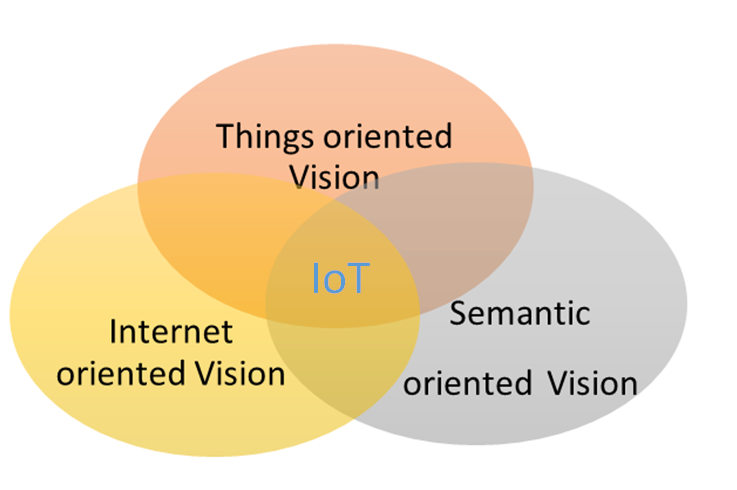
\includegraphics[width=1\textwidth]{resources/images/vision}
    \caption{Convergence of various visions of IoT adapted from~\cite{semanticiot} }\label{fig:contrib2:vision}
\end{figure}

From the perspective of "Things," the focus of IoT is on how to uniquely identify every object using specifications of the Electronic Product Code (EPC). Those objects are any things traceable using sensors and RFID technologies. Therefore, this vision depends mainly on sensor-based networks and RFID-based sensor networks~\cite{vision2}.\par
While the perspective of "things" aims at integrating various objects into a common framework, the perspective of "Internet" focuses on making smart objects interconnected. Since IP is a lightweight protocol that already connects a large number of communicating devices, it is used as well to connect heterogeneous objects~\cite{vision2}. In this context, the sensor-based object can be identified by an understandable format. This format is then uniquely identified, and its attributes are monitored as needed. \par
As mentioned earlier in this section and the previous chapter, semantics are also proposed as an IoT vision. This vision aims at providing interoperability between things in the IoT. Here is needed a general vision of processing the raw data into meaningful data and of a sealed detachment of data and their interpretation.

\subsection{Generic Architecture of IoT}

The implementation of the IoT is based on an architecture which consists of various layers. The application and business layers are presented at the top of this architecture while the field of perception layer is presented at the bottom. In this context, each component of the modern society--such as industries, enterprise, societies, institutes, and governments--is able to design the layered architecture of the IoT according to their requirements. Generally, the generic layered architecture for IoT is divided into five layers as shown in Figure~\ref{fig:contrib2:layer}. The layered architecture presented herein is proposed in~\cite{res1} and ~\cite{res2}.
\begin{figure}[htbp]
    \centering
    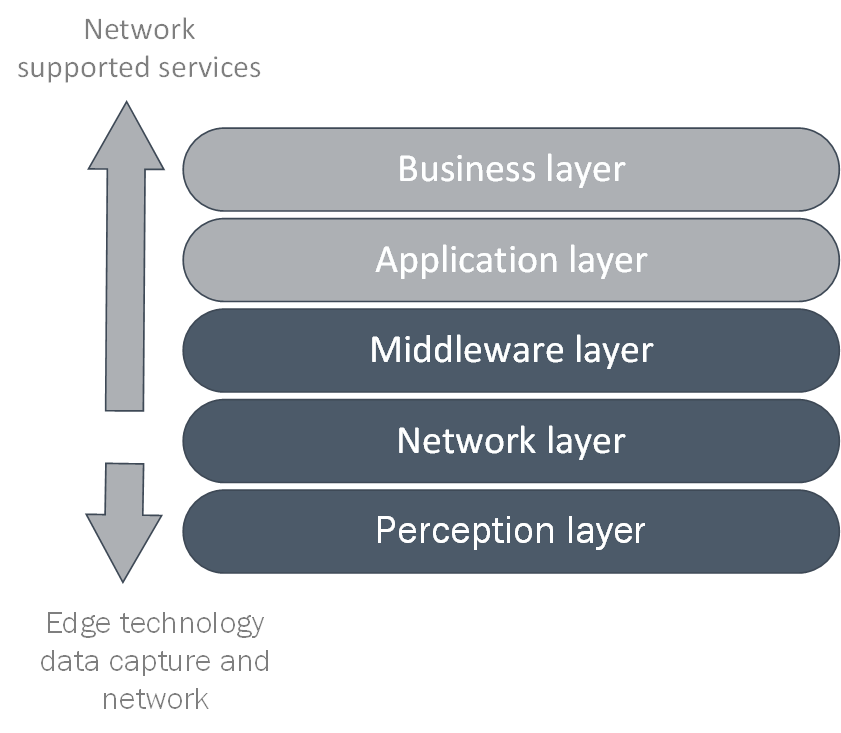
\includegraphics[width=.9\textwidth]{resources/images/iotarchi}
    \caption{The IoT Architecture inspired from~\cite{hindi} and~\cite{rep2}}\label{fig:contrib2:layer}
\end{figure}

The functionalities of the different layers are presented briefly in the following:
\begin{itemize}
\item \textbf{Business Layer:} Since that the real IoT technology success depends mainly on the business model in use, this layer is responsible for building business models, flow charts, and graphs based on the various data received from the Application layer. From this perspective, this layer has a significant role in determining the business strategies and future actions~\cite{archi}.
Application Layer: This layer represents all the different set of Application implemented by the IoT such as e-health, smart home, intelligent transportation system, etc. In a nutshell, this layer is responsible for managing applications based on the information retrieved from the set of objects processed in the Middleware layer.
\item \textbf{Middleware Layer:} This layer is responsible for managing the various services of the devices connected to the IoT system where each device is implementing a different type of service. It also stores the information and data received from the Network layer.\par
\item \textbf{Network Layer:} This layer is responsible for transferring the information and data provided by different devices and sensors from the Perception layer to the Middleware layer. In this context, the transmission medium can be wireless or wired. It also can be through various connectivity technologies such as Wifi, Bluetooth, ZigBee, etc.  
\item \textbf{Perception Layer:} This layer is responsible for the identification and collection of accurate information of sensor devices. This information varies depending on the sensors type. It can provide location, temperature, humidity, motion, etc. Afterward, this layer transfer that information to the Network layer.
\end{itemize}
\subsection{Standardization}
As presented previously, in IoT there are various technologies and components involved in data processing that have a particular data format and use different protocols. These factors make the exchange of data and communication among interconnected elements, with the intention of a combined processing of the information, a very complex task~\cite{booksd}. Therefore it is necessary that data representation, protocols, and interfaces are standardized. \par 
From this point of view, standards in IoT should be designed to meet the requirements of a various range of industries, societies, and even individual users. The design process should focus on enabling a bidirectional communication and information exchange between things. It should also emphasize their environment more and their representation in the virtual cloud from where diverse IoT applications are able to monitor, control, and assist them. As a result, standards in IoT should be created not only to support a broad range of applications but also to consider the network capacity as well as the energy efficiency~\cite{hindi}.  It is also necessary to take various regulations into consideration while designing a standard for IoT and to ensure sufficient capacity for expansion. \par
In this regard, designing a standard specified for IoT faces the interoperability issue as well. Therefore, IoT standard should ensure global interoperability between things that make use of radio spectrum in IoT. \par
In this context of IoT paradigm, at large, it is evident that the standardization of IoT is a fundamental part of the future Internet definition. This statement was already made by the cluster of European research and development projects on IoT (CERP-IoT)~\cite{fromhindi}.\par
From this perspective, there are various exciting standardization efforts being carried out by different governments and the private sector. The most relevant standardization efforts of the IoT that provide means in its design to solve the interoperability challenge are considered in the next section.

%Standards should be designed to support a wide range of applications and address common requirements from a wide range of industry sectors as well as the needs of the environment, society and individual citizens. Through consensus processes involving multiple stakeholders, it will be possible to develop standardized semantic data models and ontologies, common interfaces and protocols, initially defined at an abstract level, then with example bindings to specific cross-platform, cross-language technologies such as XML, ASN.1, web services etc. The use of semantic ontologies and machine-readable codification should help to overcome ambiguities resulting from human error or differences and misinterpretation due to different human languages in different regions of the world, as well as assisting with cross-referencing to additional information available through other systems.
\section{Standards For The Internet of Things }\index{Related Area 2}
Based on the understanding of the vision, architecture and the standardization mechanism of IoT provided in the previous section, this section focus on the organizations works on standardization process of IoT. Accordingly, this section covers only the standards that provide a definition for IoT and work on IoT as well.

\subsection{OPC Unified Architecture}

Based on the knowledge gained from the previous section, in order to realize the vision of IoT, it is required to create a global communication standard for the central components. Furthermore, it is required as well as to provide a means to manage bi-directional communication by enabling a publish/subscribe model for the low resource and a secure connection adapted for the client/server communication model~\cite{bookua}. This bi-directional communication is intended to send various commands to actors. Moreover, information is supposed to be accompanied by semantic information that represents the data and its purpose, which guarantee the best usage of the data. From this perspective, the Open Platform Communications (OPC) created a standard called Unified Architecture (OPC UA), which offers a solution for those requirements on the vertical layers for remote device access.

OPC Foundation provides various standards for data exchange, such as OPC DA specification for accessing current data, OPC HDA for accessing historical data, and OPC A&E for accessing alarms and events. The latest standard created by the OPC is the OPC UA. This standard was originally formed to enhance the Classic OPC with data modeling capabilities by providing a common, object-oriented paradigm for all OPC data~\cite{bookua}. As specified by this standard, the transport of data is mainly done by using web services based on various standards such as SOAP and HTTP or by using an optimized binary TCP protocol~\cite{bookua}. \par

OPC UA builds on the data transportation and information modeling. Thus, it aims at providing interoperability and platform-independency in the communication between applications by providing different possibilities to expose the semantics of the data provided by the Classic OPC~\cite{bookua}. One type of data provided by the OPC is the pressure measurement measured by a pressure sensor. Using the OPC UA standard, it is possible to present information in addition to the data provided by the Classic OPC. Thus, it is feasible to provide information about the type of sensor device that provided the measured temperature. This information is exposed within the OPC AU standard in a hierarchy specified for device types. Hence, OPC UA clients are capable of retrieving the information of the devices they are dealing with~\cite{bookua}. From this perspective, OPC UA provides means for different clients to process highly advanced tasks by interpreting the semantics of the provided data. \par
The OPC UA specifications provide the infrastructure to the information model. Those specifications are created to facilitate the lives of OPC UA clients by providing specifications usable by different vendor-specific OPC UA servers~\cite{bookua}. Currently, the OPC Foundation is working on defining the base model that presents the device information.\par
\subsubsection{Information Modeling}
 Based on the understanding of the previous section, the OPC UA standard is about information and data modeling. From this point of view, within this section the base principles of information modeling in OPC UA are highlighted in the following:
\begin{itemize}
\item \textbf{The use of object-oriented techniques:} those techniques which include type hierarchies and inheritance allows clients to handle all the various instance of the same type in the same way. Moreover, using the type hierarchies provide means to the user to work with the types needed and ignore the more specialized information.
\item \textbf{Accessing the type information the same way as instances:} by exposing the type information provided by the OPC UA server it is possible within the OPC UA standardization to access them in the same way as accessing instances. 
\item \textbf{Connect information in different ways:} OPC UA allows the connection among various information using a broad-meshed network of nodes. The OPC UA standard enables the use of different hierarchies exposing different semantics and references between nodes of those hierarchies. From this perspective, depending on the use case, it is possible to organize the information as needed. 
\item \textbf{Extensibility:} When it comes to information modeling, it is possible to extend the functionality of OPC UA by using various methods. In this context, it is possible for example to specify additional types of references defining relations between nodes and the definition of new methods that extends the functionality of OPC UA.
\item \textbf{Unlimited possibilities to model information:} Instead of mapping the model information to a different model, the OPC UA provide an unlimited methods to uniquely model information.
\item \textbf{Information modeling in server side only:} The information modeling is always performed on an OPC UA servers, and not on client-side. In the other hand, it is possible to manipulate them from more than one OPC UA clients.
\end{itemize}
\subsubsection{OPC UA Architecture }
he OPC UA architecture is based mainly on the communication stack between a server and the client(s). The purpose of this communication stack is to ensure encoding and decoding message requests and responses between the server and the client. Additionally, various communication stacks are able to work together only if they have the same technology mapping. This architecture is illustrated in Figure~\ref{fig:contrib2:ua}.\par
\begin{figure}[htbp]
    \centering
    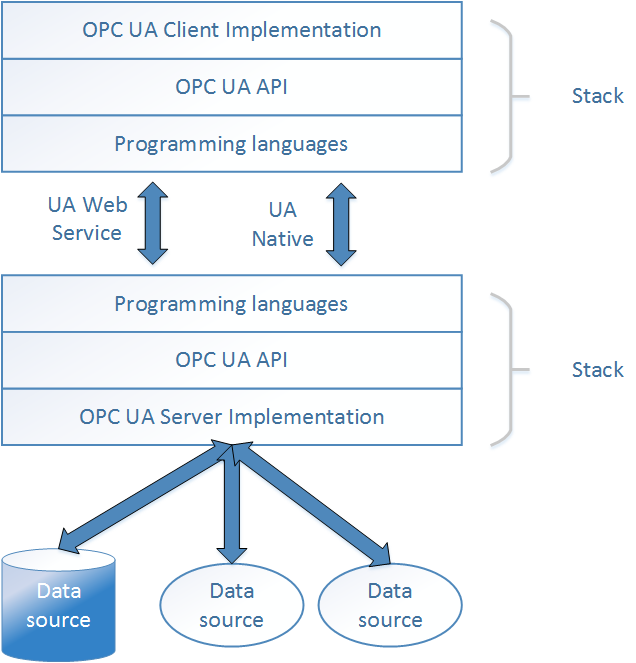
\includegraphics[width=.7\textwidth]{resources/images/OPCUA}
    \caption{The OPC UA Architecture inspired from~\cite{ua2}}\label{fig:contrib2:ua}
\end{figure}

In this context, an OPC UA client is implemented as an OPC UA communication stack. Since the OPC UA API used for accessing the communication stack can change from one operating system to another or from one programming language to another, it was not standardized. On the other hand, the client implementation should use it to access the stack~\cite{ua2}. Consequently, it is possible to develop a customized communication stack with a specific API.  \par

From the server's point of view, it is mainly responsible for delivering the request messages to the Server Implementation through an OPC UA API. This API might be the same as the API located in the OPC UA client. After receiving the request, the Server Implementation implements the logic required for returning an appropriate response message to the originator. Furthermore, as illustrated in the figure~\ref{fig:contrib2:ua}, it is possible for the OPC UA Sever Implementation to get the data from various underlying systems such as a configuration database or set of devices.\par 
Moreover, the OPC UA  aims to be more open for the different technologies used to develop an application, by defining services and concepts in an abstract manner. In this context, OPC UA specifies a technological mapping for implementation. The specified mappings address three main important tasks:
\begin{inlinelist}
  \item data encoding
  \item securing the communication and
  \item transporting the data.~\cite{bookua}
\end{inlinelist}
Currently, the OPC UA standard specifies two different mappings technologies: UA Web Services and UA Native~\cite{ua2}. While the first mapping technology uses SOAP, the second one uses only a simple binary network protocol. The OPC UA provides the possibility to encode the data. There are mainly two encoding approaches which can be adopted. Either by using XML or by using UA Binary. Each technique has advantages and disadvantages, but they are out of the scope of this thesis because the encoding of the data is independent of the mapping technologies.  \par 
Both of the approaches uses different protocols for mapping. The UA Web Service employs the SOAP/HTTP protocol while the UA Native mapping works on TCP/IP.  \par 
Furthermore, the OPC UA specification defines a concept for servers aggregation. Thus, an aggregating server is formed of one or more OPC UA server and publish the information on those servers. In this context, the client does not have to access each time multiple servers. Instead, it is able to access only one server that aggregates all the server needed.

\subsection{OMG Data Distribution Service}

The Data Distribution Service (DDS) is created by the Object Management Group (OMG) as a middleware protocol and API standard for the loT in order to enable interoperability among the connected things such as machines, mobile devices, and enterprise systems. This standard defines a data-centric connectivity by integrating the various components of a given system together in the aim of providing reliability, scalability and low latency data connectivity. It is possible to deploy the DDS standard on various platforms such as devices or the cloud. \par 
To ensure this flexible and modular structure, DDS decoupling location, time, message flow and platform from each other. This is mainly done by providing various methods. For decoupling the location, the DDS standard presents the anonymous publish/subscribe model. It also decouples the time from the other components by ensuring a time independent data distribution. Additionally, the DDS standard offers a data-centric connection management based on messages which allow the decoupling of the message flow among the different components of the system\cite{ssd2}. Finally, the DDS decouple the platform is done by supporting a platform independent model which is responsible for mapping the various models presented according to their platform. \par 
As illustrated in the figure~\ref{fig:contrib2:dds} the DDS standard define specific entities for communication and the relation between them. Those entities are described in the following:
\begin{figure}[htbp]
    \centering
    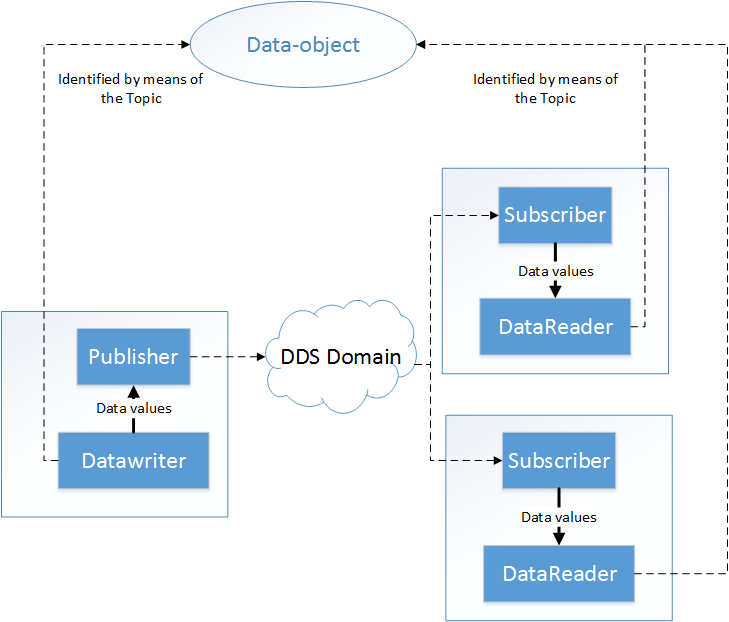
\includegraphics[width=.9\textwidth]{resources/images/dds}
    \caption{Overview of the Data Distribution Service standard inspired from~\cite{ssd} and~\cite{ssd3}}\label{fig:contrib2:dds}
\end{figure}
\begin{itemize}
\item \textbf{Domains:} the first entity is the domain which represents a virtual global data-space~\cite{ssd3} which provide information in a specific domain. Those information are accessible by all the application registered to the information domain.
\item \textbf{Publisher:} as defined in the DDS specification, the publisher is a well-defined object that is responsible for the distribution of different types of data.
\item \textbf{DataWriter:} for applications to communicate with a publisher they must use the DataWriter object. In this manner, when an application connects to a specific Publisher thought a DataWriter, the publisher should perform the distribution of data.
\item \textbf{Subscriber:} In contrast to the publisher, the subscriber is the entity responsible for receiving the published data. The subscriber is responsible as well for making the received data available for application. 
\item \textbf{DataReader:} it is required for the application to use the DataReader object in order to access the data received by the subscriber. From this perspective, subscription is defined by the a the association of a data-reader with a subscriber  which provide information about the intention of the application and which data it require in order to perform a subscription~\cite{ssd} 
\item \textbf{Topic:} This entity is used in order to make it easier for the subscriber to refer the required publication unambiguously. Thus, this object is defined to fit between publications and subscriptions.
\end{itemize}


\subsection{OneM2M Partnership Project}

OneM2M is a standard partnership project founded in 2012 by seven development organizations (SDOs) including TTA, ETSI, TIA,  ATIS,  TTC, ARIB, CCSA, and TDSI. Those participating organizations are working under the same objective which consists of transferring all standardization activities in the scope of IoT service layer to the oneM2M~\cite{onem2mC}. From this perspective, oneM2M standard partnership project aims at providing a single horizontal service platform for exchanging, sharing and manipulating data between various IoT applications which can be used in IoT industries by enabling smarter IoT services to users. Therefore, the oneM2M standard is creating various scalable and interoperable IoT standards to define the communication among things and services.\par 

OneM2M has been developing several specifications in the aim at enabling interoperability and inter-working. In contrast to the OMG Data Distribution Service and OPC UA standards, oneM2M is the only standard that developed a specification for enabling Semantic technologies to face the interoperability problem. In fact, Semantic technologies are specified by oneM2M to describe the meaning and information gathered from the oneM2M resources. Currently, oneM2M is developing standard documentations dedicated to interoperability and conformance testing~\cite{onem2ms}. \par 
In this section, the functional architecture of the oneM2M standard specification is provided as well as its key feature. Afterward, the approach used for inter-working is presented. Finally, the Semantic approach specified by oneM2M is discussed.



\subsubsection{OneM2M Functional Architecture}
In August 2014, oneM2M realised its first specification with a deployable IoT solution. Within this release, there are a set of common standards functions that enable the creation of a horizontal IoT service platform which are presented herein. The motivation behind the horizontal IoT platform is to allow various providers to work with a common framework~\cite{H} \par 

OneM2M standard specification compromise three different functions as depicts in the figure~\ref{fig:contrib1:goal}. The first function is the Application Entity (AE) which implements an M2M application service logic as specified in~\cite{onem2marchi}. Each instance executed by an application service logic is named Application Entity (AE) that can be resident in some M2M nodes and more than once on a single M2M node. The second function is Common Services Entity (CSE) which represents an instantiation of common service functions of the M2M environments. It offers several different service functions such as Data Management, Device Management, Subscription Management, and Location Services. The last function is the Network Services Entity (NSE) which provides services from different networks to the CSEs. In the context of the roles of Mca interface, it provides communication between different oneM2M CSEs~\cite{onem2marchi}.
\par
\begin{figure}[htbp]
    \centering
    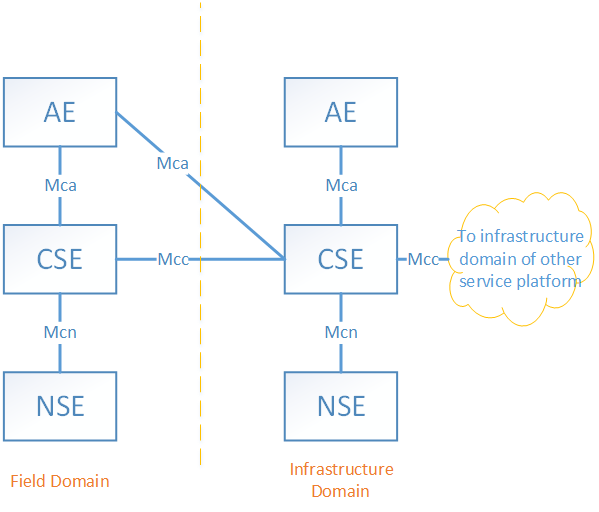
\includegraphics[width=.8\textwidth]{resources/images/arch}
    \caption{oneM2M Functional Architecture based on }\label{fig:contrib1:goal}
\end{figure}\par
There are a huge number of connected M2M and non-M2M enabled devices within an IoT network. Therefore the oneM2M standard specifies various functions to deal with this heterogeneous devices. Since that, in the modern word most of the devices connected to a given platform are more likely to face energy shortages, and they are often presented with limited storage capabilities, they can not interact immediately to all transaction with each other or with another component in the network, this situation will cause cancellation of the transaction and many other problems. Therefore, REST based architecture is considered within the the first release of oneM2M standardization. In fact, REST is based on the concept of resource addressed by URLs. Thus, it provides to the different devices connected to a given oneM2M system a way to store their states and data. In this manner, Applications that perform various transactions are able to use the internal subscription/notification mechanism specified by oneM2M to subscribe to a targeted resources and get notified by the CSE whenever the data is available or updated. An example of the oneM2M resource tree is illustrate in Figure~\ref{fig:contrib1:tree}. In this context, each device in the M2M system is presented by a uniquely addressable resource in the hierarchical tree. For example, a device can be presented by a <device\textunderscore name> resource under the hosting getaway resource <CSEBase>. Application in the other hand is presented by <Container> resource that includes one or more resource type container to classify different <contentInstences> resources under it, where the targeted data are generally located.\par
\begin{figure}[htbp]
    \centering
    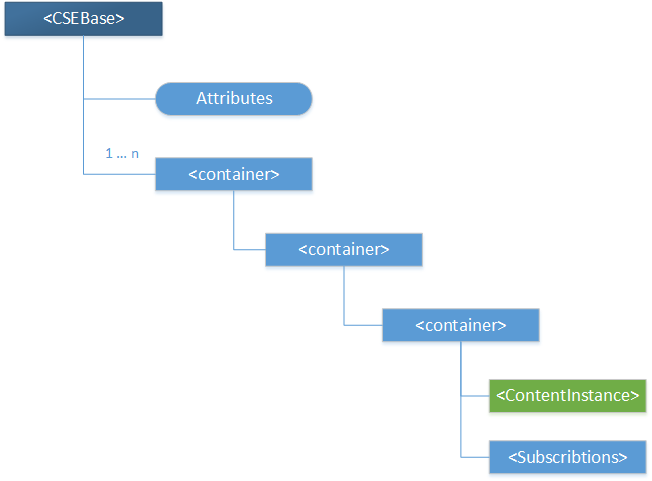
\includegraphics[width=.8\textwidth]{resources/images/tree}
    \caption{M2M Resource Tree based on oneM2M specifications}\label{fig:contrib1:tree}
\end{figure}
Moreover, the oneM2M standard specify as well a publish/subscribe architecture, which facilitate the exchange between sensor networks and cloud-based networks. The publish/subscribe architecture presents a dynamic network pattern to deliver sensor driven processed data to subscriber. It also create a decoupling communication between publisher and subscriber based on time, space and control flow. (Add Request Routing)\par
An interworking proxy entity is introduced to interconnect various local connectivity protocols

\subsubsection{Interworking Proxy Entity}
In order to provide means for interworking with non-oneM2M enabeled devices which generate a huge amount of data, the oneM2M standardization introduce an interworking proxy entity (IPE) to interconnect different local connectivity protocols such as ZigBee or ICE. As illustrated in the figure~\ref{fig:contrib1:goal}, the interworking proxy entity is defined by oneM2M as a specialized AE for interworking with non-oneM2M system as showing in the figure. IPE includes two main functionalities:  
\begin{itemize}
\item translate a non-M2M interface non-oneM2M protocols and massages to oneM2M ones via the Mca interface
\item Mapping non-oneM2M data models into oneM2M resources, which are eventually exposed to oneM2M services.
\end{itemize}\par
In this context, for each new local connectivity protocol a dedicated IPE should be created. 
\begin{figure}[htbp]
    \centering
    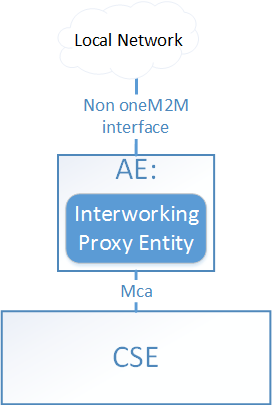
\includegraphics[width=.4\textwidth]{resources/images/ipe}
    \caption{The Interworking Proxy Entity}\label{fig:contrib1:goal}
\end{figure}
\subsubsection{Semantic Interoperabiltiy Enablement in OneM2M}
The oneM2M architecture provides procedures to discover the different resources available in a specific CSE within a given M2M system. This procedure is knowing as the resource discovery procedure (TS-0018). It is mainly processed using the RETRIEVE method which retrieves the information presented or stored in the resource's attributes. This can be done by sending a request from a specific originator (e.g. CSE or AE) to a given receiver by including the name of the target attribute in the Content parameter in the request message. When receiving the request, the receiver verifies the presence of the requested resource and checks the originator privileges for retrieving the information related to the resource. The Receiver returns the requested information only if the verification is successfully done. Otherwise, an error is returned instead. Figure TS-0018 present the mentioned procedure for retrieving a given resource.\par
Moreover, as specified in oneM2M-TS-0001 oneM2M Functional Architecture version 3, the usage of the resource discovery procedures can be customized with specified Filter Criteria parameter which limits the scope of the results. To be more specific, the filter criteria parameter provides rules description for resource discovery, (e.g. creation time, resource types, etc.).\par
Using the conventional oneM2M service layer mechanisms together with the filter criteria can provide effective resource discovery, however, it is not as advanced as expected for querying resources. Therefore, the second release of the oneM2M standard specification aims at realizing semantic-based query by annotating the target resources semantically. OneM2M enable the semantic technologies within a given oneM2M system by adding as a child resource the semantic representation of the parent resource. In this manner, all the resources provide a specific semantic representation which allows more advanced query based on semantic.\par
As defined in the oneM2M specification documentation TR-0007-Study on Abstraction and Semantics Enablement version 2.9, the type of the resources aiming at providing a semantic representation of target resources, is <semanticDescriptor> which will be discussed in more details herein. This type of resources allows the storage of the semantic description which includes relationship and information of a given resource in its child resource. Storing the different semantic information in the <semanticDescriptor> resources allows the extraction and the storage of this information in a semantic repository. The semantic repository contains mainly a set of triples allowing semantic-based query execution. The main architecture of the semantic annotator instance or the resource type <semanticDescriptor> consist of associating this type of resources with the resources that is included in it's tripled. \par
\begin{figure}[htbp]
    \centering
    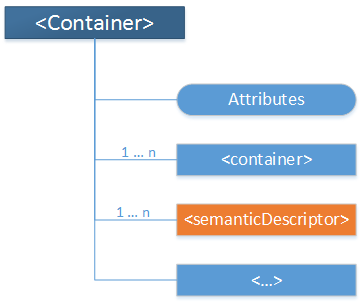
\includegraphics[width=.5\textwidth]{resources/images/sdresource}
    \caption{oneM2M Resource Tree including resource type < semanticDescriptor> }\label{fig:contrib1:goal}
\end{figure}

\sidenote{Integration}
According to the oneM2M specification, each resource in the M2M system includes one or more attribute. This attributes comprises information pertaining to the resource. Moreover, each attribute has a unique name that belongs only to a given resource and value. The resources attribute are uniquely addressable as well.\par  %In the table, a set of common attributes of M2M resources is presented. 
In the oneM2M standard specification, those attributes are commonly used by all announced resources including the resource type semantic descriptor. Besides the common attributes, there are more specific attributes for the semantic descriptor. Those attributes are shared by all announced < semanticDescriptor > specializations.\par
As specified in oneM2M TS-0004 Service Layer Core Protocol Version 2.7.1, semantic descriptor resource includes five mandatory and optional attributes as showing in the figure.
\begin{figure}[htbp]
    \centering
    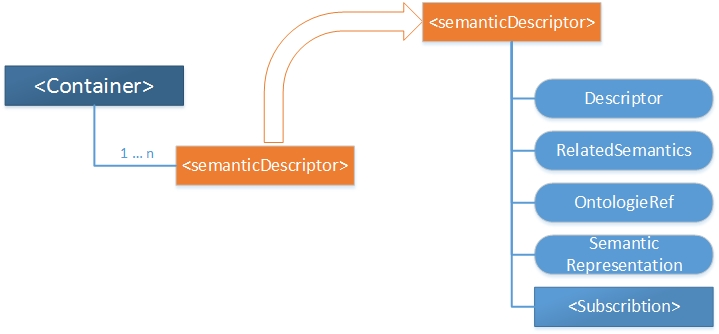
\includegraphics[width=1\textwidth]{resources/images/sdattribute}
    \caption{Structure of <semanticDescriptor> resource }\label{fig:contrib1:goal}
\end{figure}
\subsubsection{Mandatory attributes}
Mandatory attributes mean that in case one of this attributes is missing while creating the resource type semantic descriptor, an error would be throwing back, and the creation of the resource is abandoned.
Those attributes are: 

\paragraph*{Descriptor attribute:}

Each semantic descriptor must provide exactly one descriptor attribute. This attribute is responsible for storing the semantic description of the resource whose child resource the <semanticDescriptor> resource is. As mentioned previously, a semantic description is mainly provided by different ontologies within the semantic annotator architecture. More specifically this description shall be according to subject-predicate-object triples as defined in the RDF graph-based data model [4]. The encoding of the RDF triples used in oneM2M is xs:base64Binary as defined in oneM2M TS-0004 Service Layer Core Protocol Version 2.7.1[TS-0004]. Base64Binary is a representation of arbitrary Base64 encoded binary data. To be more specific data in the base64Binary format are encoded using Base64 encoding defined in RFC 4648 [9], which is derived from in RFC 2045 [10].
\paragraph*{RelatedSemantics attribute:}

For creating a new semantic descriptor resource about a resource and potentially subresource within the semantic annotator design, the semantic descriptor resource must contain exactly one related Semantic attribute. As indicated in its name this attribute provide a list of URIs for resources containing related semantic information to the resources where it was created. The URI(s) aims at referencing other <semanticDescriptor> resources. This attribute is importance because it provides means to execute SPARQL queries. This attribute will be presented and explained in more detail in the data access section.
\paragraph*{DescriptorRepresentation attribute:}
Each semantic descriptor must provide exactly one DescriptorRepresentation attribute. This attribute specifies the serialization type of the descriptor attribute. It has a fixed value application/rdf+xml:1 which consist of a string composed of a media type followed by an m2m:encoding separated by ":" character. 
\subsubsection{Optional attributes}
As defined in oneM2M TS-0004 Service Layer Core Protocol Version 2.7.1[TS-0004], resource of type <semanticDescriptor> can have one or more optional attribute that provide further information depending on the M2M system.
\paragraph*{SemanticOpExec attribute:}
The semanticOpExec attribute contains a SPARQL update request which aims at updating the descriptor attribute. Thus, it is not created or retrieved. 
\paragraph*{OntologyRef attribute:}
 The ontologyRef attribute provide a reference URL of the ontology used to semantically describe the information that is stored in the descriptor attribute. Hence, it is highly recommended to use this attribute in case the information can be described using more than one ontology.\par
The table below summarize all the specific attributes of the semantic descriptor resource.

\begin{sidewaystable}
\centering
\caption{Attributes of the semantic descriptor resource}
\label{my-label}
\begin{tabular}{llllll}
\hline
\textbf{<SemanticDescriptor> attributes}                              & \textbf{Role}                                                                                                                                                                      & \textbf{Data type}                                                                  & \textbf{Default value}                                                    & \textbf{Mandatory}             & \textbf{Optional}              \\ \hline
\textbf{descriptorRepresentation} & \begin{tabular}[c]{@{}l@{}}specify the serialization \\ type of the descriptor\\ attribute\end{tabular}                                                                   & \begin{tabular}[c]{@{}l@{}}Semantic content \\ representation\end{tabular} & \begin{tabular}[c]{@{}l@{}}application/\\ rdf+xml:1\end{tabular} & \multicolumn{1}{c}{X} &                       \\\midrule
\textbf{semanticOpExec}           & \begin{tabular}[c]{@{}l@{}}Update the descriptor \\ attribute\end{tabular}                                                                                                & SAPRQL                                                                     &                                                                  &                       & \multicolumn{1}{c}{X} \\\midrule
\textbf{descriptor}               & \begin{tabular}[c]{@{}l@{}}Storing the semantic \\ description of the targeted\\ resource\end{tabular}                                                                    & \begin{tabular}[c]{@{}l@{}}base64Binary \\ encoded data\end{tabular}       &                                                                  & \multicolumn{1}{c}{X} &                       \\\midrule
\textbf{ontologyRef}              & \begin{tabular}[c]{@{}l@{}}Provide a reference URL \\ of the ontology used to\\ semantically \\ describe the information \\ in the descriptor attribute\end{tabular}      & URL                                                                        &                                                                  &                       & \multicolumn{1}{c}{X} \\\midrule
\textbf{relatedSemantics}         & \begin{tabular}[c]{@{}l@{}}Provide a list of URIs \\ for resources containing\\ related semantic \\ information to the\\  resources where \\ it was created.\end{tabular} & List of URL                                                                &                                                                  & &   \multicolumn{1}{c}{X}                      \\\hline
\end{tabular}
\end{sidewaystable}

\section{Semantic in the Internet of Things}\index{Related Area 3}
Based on the introduction of this thesis, it is necessary to provide the semantic information of things in order to reach the ultimate goal of the Internet of Things. This need for semantic technologies in IoT in order to discover data and resources was identified by the Strategic Research Agenda (SRA) in 2010~\cite{booksd}. During the past years, semantic web technologies gained a big attention in many fields. Besides providing an efficient solution to the interoperability problem among things in IoT, semantic web technologies has proven their capabilities to link related data as well~\cite{booksd}.\par 
Thus, using semantic web technologies at the early staged of the IoT, provide means for the future research to build the concept of Linked Open Data on the earlier integration of ontologies (e.g., lightweight ontologies) into IoT infrastructures and applications. From this perspective, within this section, an introduction to the Semantic web technologies is presented as well as the explanation of the term ontology and its uses.

%SEMANTIC IN IOT The 2010 SRA has identified the importance of semantic technologies towards discovering devices, as well as towards achieving semantic interoperability. During the past years, semantic web technologies have also proven their ability to link related data (web-of-data concept) [48], while relevant tools and techniques have just emerged [49]. Future research on IoT is likely to embrace the concept of Linked Open Data. This could build on the earlier integration of ontologies (e.g., sensor ontologies) into IoT infrastructures and applications. Semantic technologies will also have a key role in enabling sharing and re-use of virtual objects  as a service through the cloud, as illustrated in the previous paragraph. The semantic enrichment of virtual object descriptions will realise for IoT what semantic annotation of web pages has enabled in the Semantic Web. Associated semantic-based reasoning will assist IoT users to more independently find the relevant proven virtual objects to improve the performance or the effectiveness of the IoT applications they intend to use.
%2.11.4.1 IoT interoperability necessary framework
%2.5.3. http://www.internet-of-things-research.eu/pdf/Converging_Technologies_for_Smart_Environments_and_Integrated_Ecosystems_IERC_Book_Open_Access_2013.pdf

\subsection{Semantic Web technologies }
The director of the World Wide Web Consortium (W3C) and the inventor of the World Wide Web Tim Berners-Lee together with James Hendler and Ora Lassila published the first article that features the "Semantic Web" in May 2001~\cite{hi}~\cite{rb}. This article presents a novel way to use and search the Internet which can be seen as a new dimension that provides new opportunities and possibilities. Since HTML provides means to store visual information, it is rather designed for human and computers. Thus, it is not possible for computer or search engine to read and understand the text of an HTML web page. \par 
From this perspective, the Semantic Web aims at extending the current World Wide Web to focus on technology as well as human. Thus, in contrast to the World Wide Web, the Semantic Web does not require a human presence. It uses the natural languages to search compile and organize information from the Web. Therefore, the human presence in the Semantic Web is only required to initiate a request. This approach would enable, for example, machine agents to intelligently search the Web, create decisions and accomplish tasks on behalf of humans~\cite{rb}.
As illustrated in the figure~\ref{fig:contrib2:stack} the architecture of semantic web consists of various layers where each layer uses the capabilities of the layer below. 
\begin{figure}[htbp]
    \centering
    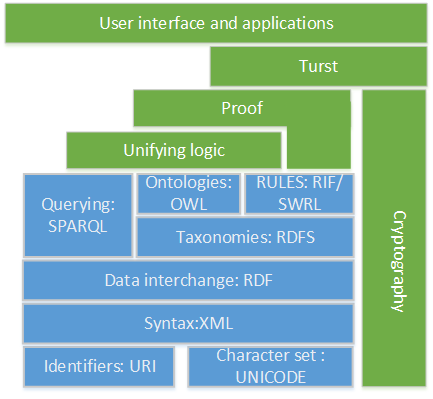
\includegraphics[width=.6\textwidth]{resources/images/stack}
    \caption{Semantic Web Stack based on~\cite{layer}}\label{fig:contrib2:stack}
\end{figure}
The bottom layers of the stack which are highlighted in blue indicate the components of the semantic web that have been standardized. In the other hand, the upper layers highlighted in light green are not clear yet how to implement them, but they are still required for a sufficient deployment of Semantic Web~\cite{layer}. \par
The first layer which consists of the URI and Unicode follows the important features of the existing Web. In fact, international character sets are encoded using the Unicode standard which allows the usage of human languages on the web. The URI refers to Uniform Resource Identifier which consists of a string of a standardized form that provides means to uniquely identify resources. The URL includes two subsets: the Uniform Resource Locator (URL) and Uniform Resource Name (URN). It is important to use URI(s) to guarantee the distribution of the Internet system~\cite{layer2}. \par 

Extensible Markup Language (XML) layer ensure a common syntax usage in the Semantic Web~\cite{layer2}. Thus, the use of XML allows the description of data in a way that is both human and machine-readable. Furthermore, XML includes various applications such as the Resource Description Framework (RDF) which is the core data representation format for Semantic Web. \par

As it was mentioned previously, RDF is the core data representation format for Semantic Web~\cite{thesis}. It is a framework that allows the description of the information in a graph form. XML and Turtle (TTL) can both be employed as the normative syntax for serializing RDF. The base of RDF is the usage of triples (subject, predicate, and object) that form a graph of data. Thus, all information in the Semantic Web is described through the RDF language. Each subject and predicate are denoted by a unique Uniform Resource Identifier (URI), generally a Uniform Resource Locator (URL). In the other hand, the object can either be a literal or a URI. From this perspective, it is possible to form a directed graph, as shown in Figure~\ref{fig:contrib2:rdf}, where objects are represented using literal and URI. Furthermore, it is possible to use RDF/XML to serialize the graph. In fact, various formats can be used for serialization such as JSON/JSON-LD, N3, and N-Triplets. There are common concepts presented by the RDF specification such as blank nodes and collections.
\begin{figure}[htbp]
    \centering
    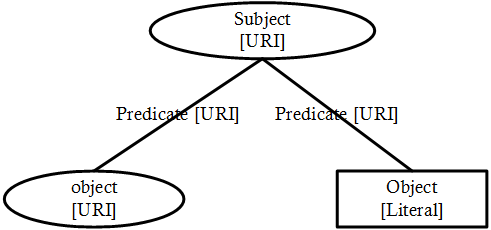
\includegraphics[width=.5\textwidth]{resources/images/rdf}
    \caption{Types of RDF triples}\label{fig:contrib2:rdf}
\end{figure}
Since that RDF provides possibilities to represents graphs formed by triples, it is possible to almost anyone to define the vocabulary of terms used for more detailed description. In this context, RDF Schema (RDFS) is created to provide a standardization for taxonomies and ontological constructs description. Thus, RDFS enable the creation of lightweight ontologies through describing taxonomies of classes and properties~\cite{rdfs}. In fact, all resources are divided into groups called classes. In the same way, classes are also resources. Therefore they are identified by URIs, and they are described using properties. Each member of a class is called instance, which is stated using the rdf:type property. Moreover, RDFS define all resources as an instance of the class rdfs:Resource, all classes as an instance of rdfs:Class and subclasses of rdfs:Resource. Concerning the properties they are defined as instances of rdf:Property which presents relations between subjects and objects in RDF triples such as rdfs:subClassOf or rdfs:label. \par
In order to create more complex ontologies, it is required to use the Web Ontology Language (OWL) which is derived from description logics. The OWL offers more constructs over RDFS by providing additional standardized vocabulary~\cite{owl}. As showing in Figure~\ref{fig:contrib2:owl}, there are three species of OWL:
\begin{inlinelist}
  \item OWL Lite for taxonomies and simple constrains
  \item OWL DL for full description logic support
  \item and OWL Full for maximum expressiveness and syntactic freedom of RDF.~\cite{owl}
\end{inlinelist}\par 
\begin{figure}[htbp]
    \centering
    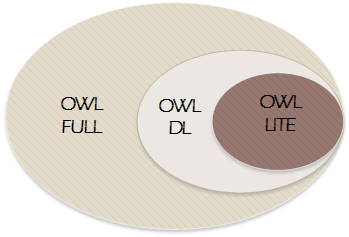
\includegraphics[width=.5\textwidth]{resources/images/owl}
    \caption{the relationships between OWL species based on~\cite{owlpic}}\label{fig:contrib2:owl}
\end{figure}
OWL Lite is the simplest OWL language used to express taxonomy and simple constraints. On the other hand, OWL Full is the most complex OWL language formed by the full OWL vocabulary~\cite{owl}. Thus it has no expressiveness constraints which allow complex expressions. OWL DL provide means to use the knowledge representation formalism Description Logics (DL) which are a family of formal knowledge representation languages used for defining general ontologies~\cite{dl}. Hence, OWL DL in one hand support maximum expressiveness, and in the other, it retains computational completeness by providing description logic capabilities. As showing in the figure~\ref{fig:contrib2:owl}, each legal OWL Lite ontology can be considered as a legal OWL DL ontology, in the same manner, each legal OWL DL ontology is seen as a legal OWL Full ontology. Generally, the inverse of this relation do not hold~\cite{owlpic}.\par 

For performing queries on RDF data, RDFS and OWL ontologies with knowledge bases, the SPARQL Protocol And RDF Query Language (SPARQL) are available[]. SPARQL is an SQL-like language used to query ontologies such as RDFS and OWL. It used RDF triples for the matching part as well as the returned results. Thus, the TURTLE syntax is used in order to express RDF graphs in the matching part of the SPARQL query~\cite{thesis}. SPARQL is considered a protocol for accessing RDF data as well.\par 
 
Based on the figure~\ref{fig:contrib2:stack}, it is expected that all the semantics and rules are performed within the layers underneath Proof. Thus, the results are used to prove deductions. The trust layer means that the proof and the trusted inputs signify that the results are trustful. Finally, cryptography is used in order to provide reliable inputs.

\subsection{The Semantic Web Technologies stack for IoT}
Figure~\ref{fig:contrib2:stack2} debate an overview on how Semantics can be used at various levels in IoT. The figure was adapted from ~\cite{stacksemantic2}in order to illustrate the Stack presented by the Semantic Web Technologies for IoT. \par 
Based on the figure, there are three main levels where the Semantic Web technologies can be integrated~\cite{stacksemantic1}. The first level is the "modeling level" which aims at providing a common understanding the capacities, characteristics, and relations of Things. Thus, integrating Semantic Web
technologies at this level enable the use of shared and accepted vocabularies and lightweight ontologies which facilitate the integration of data generated by a various system. Such an integration of vocabularies and ontologies in the "modeling level" can be done by using a sensor ontology to describe the sensor data collected. The second level is the "data processing level." Using Semantic Web technologies within this level enable reasoning and inference over the data~\cite{stacksemantic1}. To be more specific, this level requires the use of description logic and OWL semantics described in the previous section. The third level is the IoT Services and Application". Enhancing this level with the Semantic Web technologies by using specific ontologies and description enable the discovery, publication, and composition of services in IoT.
\begin{figure}[htbp]
    \centering
    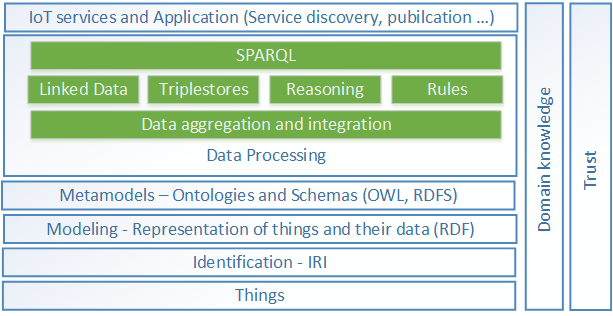
\includegraphics[width=1\textwidth]{resources/images/stacksemantic}
    \caption{The Semantic Web Technologies stack for IoT adapted from~\cite{owlpic}}\label{fig:contrib2:stack2}
\end{figure}

\section{Ontologies for the Internet of Things}

As presented in the previous section, ontologies provide a distributed and common description of various domains communicated between people and application systems. Since ontology aims at providing a consensual domain knowledge, its development involve a various cooperation between different people possibly located at different locations.\par 
In this context, there are already different projects working on ontologies and vocabularies indexation on the Web. Currently, the most popular schemas on the Web is Schema.org which is a collaborative and community work aiming at creating, supporting and promoting schemas for structured data on the Web~\cite{stacksemantic1}. At the time of writing, schema.org is used by more than 10 million sites in order to markup their pages and email messages~\cite{schema}. Although schema.org provide full descriptions for general and commonly used aspect such as Places, relationships, Person, etc., it does not provide specific IoT domain concepts such as Sensor concept.\par 

Thus, currently, many research and works aim at providing a vocabulary specified for IoT. At the time of writing, there are already 300 IoT-specific vocabularies presented in the Linked Open Vocabularies (LOV) online catalog maintained at~\cite{site}. The Open Knowledge Foundation creates the Linked Open Vocabularies in order to facilitate the research process of the various type of vocabularies dedicated for data description on the Web~\cite{rfr}. Evaluating and comparing 300 ontologies is out of the scope of this thesis and will be reserved for future work. However, the most relevant and well-referenced ontologies in other works are presented herein. \par 

One of the most well-knowing ontologies in the field of IoT is the Semantic Sensor Network Ontology (SSN) developed and maintained by the W3C Semantic Sensor Network Incubator Group in 2011~\cite{ssn}. The full ontology inherits its 41 concepts and 39 object properties directly from 11 DOLCE Ultra Lite (DUL) concepts and 11 DUL object properties~\cite{ssn}. SSN ontology is able to describe sensors, their capabilities, observations and methods for sensing~\cite{ssn}. Moreover, the SSN ontology includes various concepts for operating and a structure for field deployments which describes the deployment lifetime. This ontology is built on a central Ontology Design Pattern (ODP). This design aims mainly at describing the relationships between sensors, stimulus, and observations referred to as the Stimulus-Sensor-Observation pattern.
The SSN ontology can be presented using four different perspectives~\cite{ssn}: 
\begin{itemize}
\item \textbf{Sensor perspective:} this perspective focus on the output of the sensors, what is this output and how it was sensed. 
\item \textbf{Observation perspective:} this perspective concentrate only on the observed data and related metadata.
\item \textbf{Property perspective:} which focus on the observations that have been made about a particular property.
\end{itemize}
This ontology takes on consideration an inclusive view of what a sensor is. A sensor is defined in the SSN ontology as anything that observes. Furthermore, SSN allows for each sensor to have a hierarchical representation using ssn:hasSubSystem object property~\cite{rfr}. This representation is illustrated in the Listing~\ref{lst:contrib3:rw1}. Although SSN is considered a “5 star” ontology which follows all the rating requirements, it does not provide means to represent the concept of Actuators~\cite{rfr}. It also does not include various material such as units, locations, and hierarchies of sensor types~\cite{ssn}. \par 

\lstset{caption=An example of a System with a Temperature Sensor and a Pressure Sensor, label=lst:contrib3:rw1,
language=xml, breaklines=true, numbers=left, basicstyle=\small\ttfamily,
stepnumber=1, frame=single, inputencoding=utf8/latin1}~\lstinputlisting{resources/code/ssn.rdf}

Besides the SSN ontology, there are various specialized information models defined for the IoT such as the Zigbee or KNX data models. The SSN ontology, as well as those specialized ontologies, suffer from two main issues. Either those ontologies are too specialized to be used in different scenarios because they concentrate on a particular application domain or they lack some important concepts such as the lack of actuator representation within the SSN ontology. For those reasons, multiple ontologies are constructed from those ontologies in order to handle the missing concepts or to be more generalize to allow the usage of the ontology by different stakeholders. Thus, in this thesis, there are two main ontologies considered which are not very specialized and offer all the essential concepts for the data annotation. The first ontology considered is the Fiesta-IoT Ontology which is an EU project that comprises 14 partners and integrates previous and ongoing EU projects already using semantic web technologies~\cite{fiesta1}. Fiesta-IoT Ontology is a collection of merged concepts from different exciting ontologies such as the SSN ontology previously presented, IoT-lite, M3-lite Taxonomy, Time and DUL. The second ontology considered is the oneM2M Base ontology specified by the oneM2M standard specification in TS012~\cite{baseontology}. Since the design discussed within this thesis rely mainly on the oneM2M specification, it is more beneficial to use the ontology specified by the standard.


\section{OpenMTC Platform}

OpenMTC platform~\cite{openmtc} is an M2M solution for the Internet of Things created and developed by The Fraunhofer FOKUS and Technical University of Berlin (TUB). This platform is considered as an implementation of the oneM2M standard specification which has been designed as a horizontal layer spanning across multiple vertical domains (e.g., Smart transport, eHealth, etc.). The OpenMTC platform support integration of heterogeneous sensors which allows the applications developers to use and manipulate various heterogeneous devices and sensors. Thus, with its concept, OpenMTC platform enable academia and industry to deploy it independently or as part of a common platform.\par 

Currently, this platform is moving toward an intelligent fog node framework called OpenIoTFog~\cite{openiotfog} where the semantic interoperability is required. Therefore, this work aims at moving the OpenMTC towards the OpenIoTFog by providing semantic interoperability which can be done thanks to the oneM2M standard specification implementation within the platform. \par 
As discussed previously, the oneM2M standard specification is one of the fewer standardization efforts that follows the semantic interoperability approach by specifying methods and concepts in this regards. Hence, the OpenMTC platform is considered within this thesis as the perfect candidate for implementing semantic technologies for two main reasons. First, as mentioned in the previous paragraph, the OpenMTC platform provide various possibilities to interact and collect data from many heterogeneous oneM2M and non-oneM2M enabled sensors and devices. Thus, the interoperability problem is a real threat to the platform that should be handled. Second, the OpenMTC platform provides a full implementation of the oneM2M standard specification. Therefore it is possible to apply the semantic technologies on the platform by using the second release of the oneM2M specifications which provide a full description of the semantic implementations within a oneM2M platform. \par
This section presents an understanding of the OpenMTC platform architecture and its mains features.

\subsection{System Architecture}
The architecture of the OpenMTC platform adapts the high-level functional architecture specified by oneM2M which mainly consist of two service capability layers. A gateway service capability layer (GSCL) and a network service capability layer (NSCL). Those layers have been defined and specified by the ETSI Technical Committee M2M. The architectural design of OpenMTC run the different modules on an event based platform following the event based library concept Gevent which provide asynchronous I/O API that can scale its number of execution units according to the processing load. In Figure~\ref{fig:contrib2:openmtc}, the architecture of the OpenMTC is illustrated. As showing in the figure, OpenMTC mainly consists of a back-end M2M capability layer and a front-end M2M capability layer which follows the oneM2M standards as well as the ETSI Technical Committee. The front-end and back-end nodes are capable of using several transport protocols, such as HTTP, CoAP, and Websockets. As illustrated in Figure~\ref{fig:contrib2:openmtc}, it is possible to control the communication and interaction between the front-end and the back-end of the OpenMTC platform using the connectivity management layer over managed and unmanaged Access Networks. Thus, this layer is mainly responsible fort the communication establishment and messages forwarding. Furthermore, the core architecture of the OpenMTC platform includes the principle functionality defined by the oneM2M CSEs along with a set of application enablement APIs that allows the development of applications by third party.\par
\begin{figure}[htbp]
    \centering
    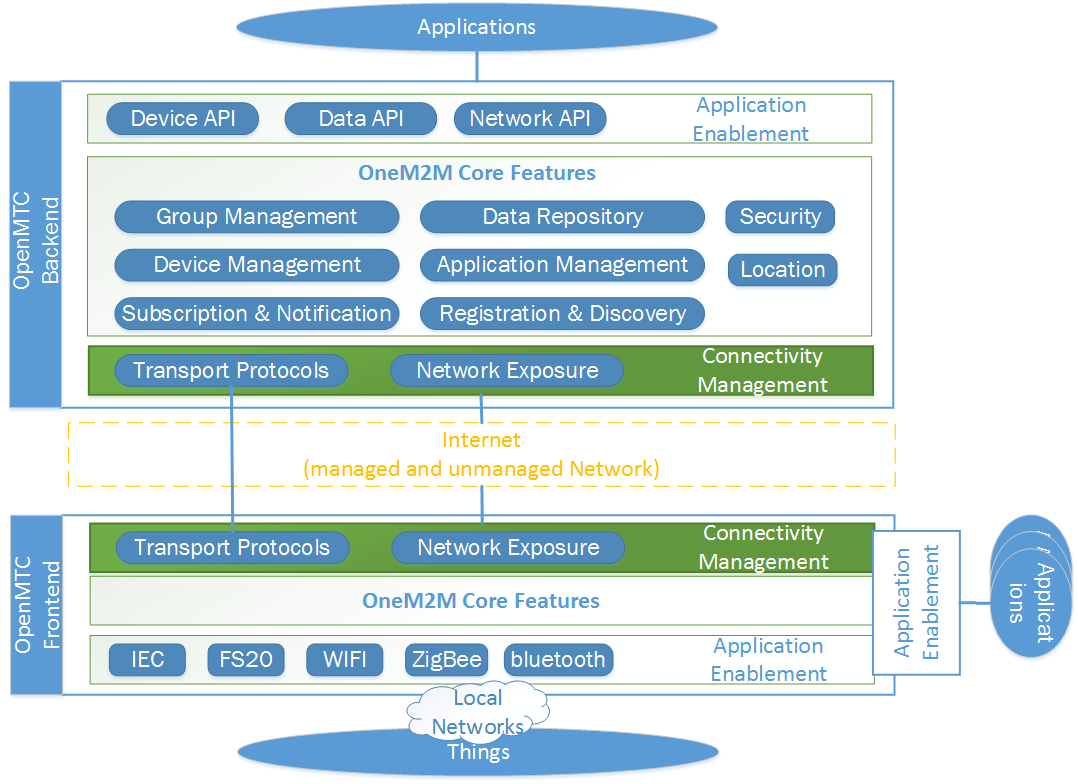
\includegraphics[width=1.1\textwidth]{resources/images/openmtc}
    \caption{The OpenMTC Platform Architecture based on~\cite{owlpic}}\label{fig:contrib2:openmtc}
\end{figure}
Furthermore, the client/server based RESTful architecture with the hierarchical resource tree defined by oneM2M are supported within the core architecture of the OpenMTC platform. Thus, using those features, it is possible for each device, sensor or "thing" to connect and store its states and data in the platform. Another characteristic of the OpenMTC platform is the separation of the communication over the platform interface and the transport protocol. Following the oneM2M standard specification, the OpenMTC platform offers a subscription and notification mechanism through its Addressing and Repository (RAR) capability which facilitate the management of the things connected to the platform~\cite{openmtc}. Using this mechanism provide various applications and services as well as the OpenMTC platform with the possibility to subscribe to a targeted resources and each time the resource subscribed to is modified they get notified.\par 
 In order to provide possibilities to interact with various heterogeneous sensors, devices or things, the OpenMTC platform provides different inter-working proxies entities that follow the oneM2M standard specification. Each IPE is responsible for one specific technology such as ZigBee or IEC which control the external devices by mapping them into the M2M resource tree structure. Thus, it is possible within the core design of the platform to integrate a specific IPE as needed.

\subsection{OpenMTC Key Features}
Based on the previous subsection it is possible to identify the key feature of the OpenMTC platform. Those features are highlighted in the following:
\begin{itemize} 
\item \textbf{OpenMTC Back-end:} There are various features provided by the back-end of the platform.  It offers a real-time data aggregation and processing as well as a well-defined device management and discovery system. As explained previously the core design of the back-end support as well different deployment scenarios. Finally and most importantly, it is possible within the openMTC back-end to develop IoT and M2M applications over a common platform. 
\item \textbf{OpenMTC Front-end:} This M2M capability layer provide various key feature as well. First and most importantly, it offers various possibility to support various sensors and actuators such as FS20, ZigBee or Bluetooth. This layer support also the use of different gateways such as Android-based gateways or Linux-based gateways.
\item \textbf{M2M Communication:} As it was mentioned previously, there are different ways of communication within the OpenMTC platform. The platform support open REST APIs and various communication protocols such as HTTP, MQTT or CoAP. The wireless access within the openMTC is supported as well.
\item \textbf{Scalable and Flexible:} The scalability of the platform is supported by its cloud-enabled deployment which is defined in one complete M2M solution. Moreover, the platform offers more flexibility through the separation of the functional elements available.
\end{itemize} 
\section{Conclusion}

\sidenote{Summary}
\todomid{write}

\sidenote{Takeaway 1}
\todomid{write}

\sidenote{Takeaway 2}
\todomid{write}

\sidenote{Takeaway 3}
\todomid{write}

\sidenote{Next chapter}
\todomid{write}
The idea behind this approach is to both optimize the query execution process and also to provide a way to perform a semantic query on the discovered semantic descriptors presented in the hierarchical resource tree without requiring the creation of a local temporary semantic graph store to put all the semantic triples extracted from the targeted resources.
    \cleardoublepage
\chapter{Requirement Analysis}\label{sec:reqs}\minitoc\vspace{.5cm}
\index{Requirements}

\section{Introduction}

The previous chapter presented an overview of state of the art in the field of semantic interoperability in the Internet of things with a focus on providing an M2M system with the semantic capabilities to overcome the interoperability issue. Based on this overview and in order to elaborate on the research issues in the dissertation, this chapter identifies the requirements for the implementation of the Semantic annotation extension which aims to provide a given M2M or IoT system with the semantic capabilities. \par 
All requirements can be separated into functional and non-functional[add roben reference].The former are concerned about the actual scope of operation, whereas the latter mainly focus on how the system should behave and perform.

\section{Functional Requirements}
The following functional requirements specify the essential functions of the Semantic Annotation Extension designed and implemented within this work. Those requirements are primarily categorized according to fundamental semantic aspects which are listed herein in sort of their relativity to the thesis objectives. 

\subsection{Semantics Annotation}
As it was discussed in the previous chapter, the main objective of this work is to provide interoperability between things in an M2M system. Those things can be presented as sensors, actuator or devices that communicate with the platform using a various set of technologies. Furthermore, in an M2M system complying with the oneM2M specification, those things are mapped to a oneM2M hierarchical resource tree. In this manner, each resource has a representation that can be transferred and manipulated with CRUD methods such as Create, Retrieve Update and Delete. \par 
From this perspective, the Semantic Annotation Extension shall provide capabilities to a given M2M system to manage semantic information about the oneM2M resources by adding and representing the semantic of those resources that shall be made available in a given M2M System for advanced semantic operation such as Semantic Query or semantic discovery of the resources. Thus, the Semantic Annotation Extension shall support a common language for semantic description such as RDF. 

\subsection{Ontology Specification}
Ontologies play a central role in enriching data with a conceptual semantics. From this perspective, the Semantic Annotation uses ontologies to index the content of the M2M resources which can result in the representation of explicit knowledge. In the other hand, as it was presented in the State of the art, the number of ontologies that are being built and already in use is growing fast. \par 
Moreover, not all the ontologies available can be used to annotate the resources' content. From this point of view, The following list of Ontology requirements should be fulfilled in order to provide an efficient Semantic Annotation:
\begin{itemize}
\item In order to semantically annotate M2M resources, the system shall use an ontology for IoT that represents a variety of specific concepts.
\item As it was previously presented the number of ontology already in use or being built is growing[], hence each stakeholder may use a specific independent ontology leading to a deepening of the interoperability problem. Therefore the semantic annotation extension shall provide the possibility to annotate data and information using a different set of ontologies and not to rely only on one ontology.
\item Based on the second requirement description, the system shall provide the possibility to annotate the resources' content using more than one ontology simultaneously and the possibility to add or remove and ontology annotation as needed.
\item The Semantic Annotation Extension shall provide means to extend ontologies in the M2M system.
\item The Semantic Annotation Extension shall be able to support updating, managing and discovering ontologies within an M2M system.
\end{itemize}

\subsection{Semantic Repository}

The Semantic Annotation extension needs to provide a centralized location particularly for semantics to a given M2M system such as a Semantic Repository. The Semantic Repository shall contain all the information extracted from the resource semantics instances. Thus, Information stored in the Semantic Repository are then available via an SPARQL endpoint.

\subsection{Semantics Query}
The Semantic Annotation Extension shall enrich a given M2M system with the capabilities to discover M2M resources using semantic descriptions. Thus, the applications and users can perform a semantic operation on the M2M resources.

\section{Non-Functional Requirement}
As it was presented in the introduction of this chapter, The non-functional requirements listed below, elaborate a performance characteristic of the system. They are not as many, yet they are critical as well.
\subsection{Semantic Interoperability}
Semantic interoperability is a key indicator of this work. Thus, based on the knowledge gained from the previous chapter, the interoperability is the main aim of this thesis which would provide interoperability between heterogeneous devices and services in a given M2M system compliance with the oneM2M standards.
\subsection{Modularity}
Modularity can be categorized as a practical application of the principle of "Separation of Concerns"~\cite{mo}. It basically means that a complex system is divided into simpler and more manageable modules. Each module includes a set of small and basic functions dedicated for a set of specific task. \par
Modular programming is typically useful for program readability and re-usability~\cite{mo}. Thus, it is important in this dissertation because it offers the possibilities to divide the Semantic Extension Implementation into a set of modules where each module is responsible for a particular task. In this manner, it is more advantageous to update the Ontology implemented or extend it by just updating or modifying the module in charge of the ontology. Also, this requirement may facilitate the integration of the semantic Extension within a given M2M system.
\subsection{Usability}
In this context usability refers to the adaptation of the M2M platform's users (e.g. Application, developers) to the Semantic annotation usage. Hence, it should be easy enough for the user to perform and execute semantic operation within a given M2M system such as SPARQL Query operation or resource discovery based on Semantic description.\par  
Moreover, the users shall be able to choose more than one ontology for data and information annotation in a flexible and simultaneous manner.
\subsection{Performance}
 Performance measurements provide key indicators to estimate the quality of a developed solution. They are used mainly to quantify specific characteristics of a system. In this context, the performance of the oneM2M extension should be reflected in reasonable times for carrying out Semantic Operations, the potential for scalability and the quality of the data and information annotated simultaneously using a set of ontologies.
 \subsection{Security}
 Since that the use of semantic provide additional methods to the M2M users and applications for advanced discovery requests based on semantic such as an SPARQL Endpoint, the oneM2M security solutions should be enhanced. This can be done by rebuilding the authorization mechanism. Although this requirement is of a recognizing importance, it is not in the scope of this thesis. 

\section{Conclusion}

The functional and non-functional requirements for the design and implementation of a Semantic Annotation Extension in a given M2M system are presented within this chapter. Some of those requirements is already defined in oneM2M TS-0002~\cite{02} and adapted to this work. In the given table~\ref{f}, The functional as well as non-functional requirements are prioritized according to their importance for a working working prototype of the Semantic Annotation Extension.

\begin{table}[htbp]
\centering
\caption{Prioritization of functional requirements}
\label{f}
\begin{tabular}{*{14}lll}
\hline
\multicolumn{1}{}{\textbf{Requirement}} & \multicolumn{1}{}{\textbf{Priority}} & \multicolumn{1}{}{\textbf{}} \\ \hline
Semantics Annotation                      & major                          &                                \\\hline
Ontology Specification                    & major                                   &                                \\\hline
Semantic Repository                       & major                                   &                                \\\hline
Semantic Query                            & minor                                   &                               
\end{tabular}
\end{table}

As presented in table~\ref{f}, there are two possibilities to prioritizes a requirement. Either by using \textit{major} which means that the requirement is critical for the implementation  or by using \textit{minor} which mean that the specified requirement is of relevant but not essential for the implementation.\par 

The methodologies used to specify, which requirement should be marked as \textit{major} and which not, can be understood as follow: all requirements that are mandatory for semantically annotate the information and targeted data should be marked as \textit{major}, in the other hand the requirements that does not affect the functions for the integration are seen as complementary. Thus the latter are marked as \textit{minor}. \par 

The same process is elaborated with the non-functional requirement which is illustrated in table~\ref{f2}. \par 
\begin{table}[H]
\centering
\caption{Prioritization of non-functional requirements}
\label{f2}
\begin{tabular}{*{14}lll}
\hline
\multicolumn{1}{}{\textbf{Requirement}} & \multicolumn{1}{}{\textbf{Priority}} & \multicolumn{1}{}{\textbf{}} \\ \hline
Semantic Interoperability                 & major                                 &                                \\\hline
Modularity                                & major                                   &                                \\\hline
Usability                                 & major                                   &                                \\\hline
Performance                               & major                                   &                                \\\hline
Security                                  & out of scope                            &                               
\end{tabular}
\end{table}
There is a new prioritization term used within the table~\ref{f2}. Out of scope means that the specific requirement is not in the scope of the thesis. Thus, as it was discussed in this chapter the security requirement is left out of the thesis objectives.
    %\cleardoublepage
\chapter{Design and Specialisation}\label{sec:contrib1}\minitoc\vspace{.5cm}
\index{Contribution 1}

\section{Introduction}
\sidenote{Overview}
As outlined in the introduction, the goal of this thesis is to design and implement a semantic annotation extension of the OpenMTC Platform aiming to provide semantic interoperability for accessing resources and interpreting data from different stakeholders. This goal is a part of the overall goal of the IIoT department which aims at moving the OpenMTC platform towards an intelligent Fog Node framework (OpenIoTFog).
This extension allows OpenMTC to create a pool of common data available in a specific environment and to share them between different OpenMTC applications, without requiring the information of the data type or content (units, metadata, context, etc.) in advance. Moreover, our implementation consist as well in enabling data access via SPARQL interface and OneM2M standard. The figure .1.1 demonstrate an overall picture of the whole concept.\par


\section{Overall Architecture}

The high-level functional architecture specified by oneM2M is adapted to define the detailed architecture of the semantic annotation extension. In this context, M2M middleware platforms provide huge advantages when it comes to Smart City implementations. Hence, it is expected to provide interoperability and communication between machines “things” and their virtual representation on the M2M middleware to support object addressing, tracking, and discovery as well as information representation, storage, and exchange. In this section, we specify a semantic annotation extension aiming to provide semantic interoperability within an M2M system. Figure 5.2 depicts the High-level architecture of the semantic annotation extension within an M2M service middleware. In such a oneM2M compatible system the semantic annotation extension is considered to be located in the frontend as well as the backend of the system. \par
The M2M middleware aligned with oneM2M standard specification compromise three different functions as depicts in the figure. The first function is the Application Entity (AE) which implements an M2M application service logic as specified in []. Each instance executed by an application service logic is named “Application entity” (AE) that can be resident in some M2M nodes and more than once on a single M2M node. The second function is Common Services Entity (CSE) which represents an instantiation of common service functions of the M2M environments. It offers several different service functions such as Data Management, Device Management, Subscription Management, and Location Services. The last function is the Network Services Entity (NSE) which provides services from different networks to the CSEs. In the context of the roles of Mca interface, it provides communication between different oneM2M CSEs. A description of the implemented capabilities within the prototype system is given in the next chapter. 
\par
\begin{figure}[htbp]
    \centering
    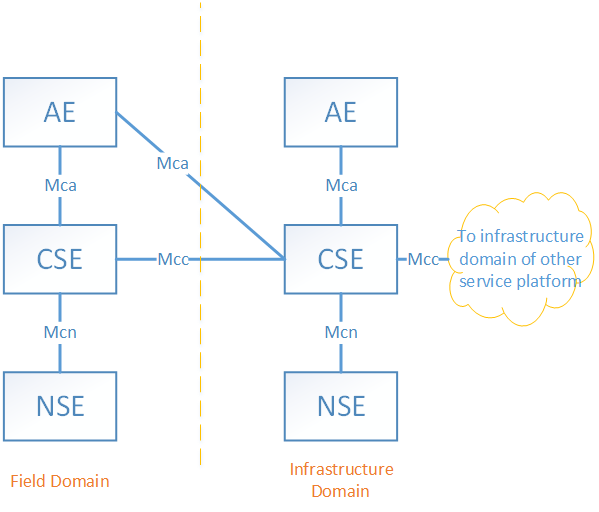
\includegraphics[width=.9\textwidth]{resources/images/arch}
    \caption{oneM2M Functional Architecture}\label{fig:contrib1:goal}
\end{figure}\par
There are a huge number of connected M2M and non-M2M devices within an M2M network. Therefore our semantic annotation extension considers different architecture designs to deal with this heterogeneous devices. Since that, most of the devices connected to the M2M network are more likely to face energy shortages, and they are often presented with limited storage capabilities, they can't interact immediately to all transaction with each other or with another component in the network, this situation will cause cancellation of the transaction and many other problems. Therefore, REST based architecture is considered within the semantic annotation extension as well as any M2M system. In fact, REST is based on the concept of resource addressed by URLs. Thus it provides to the different devices connected to the M2M network a way to store their states and data. In this manner, our semantic annotation extension makes use of the internal subscription/notification mechanism provided by the inner-API which is mainly based on events to subscribe in oneM2M system to a targeted resources. The CSE sends back notification as soon as the data is available or updated which enables the extension to get used to the targeted data. Figure illustrate the M2M resource tree evaluated in our extension.  In this context, each device in the M2M system is presented by a uniquely addressable resource in the hierarchical tree. For example, a device can be presented by a <device\textunderscore name> resource under the hosting getaway resource <scl>. Application in the other hand is presented by <application> resource that includes one or more resource type container to classify different <contentInstences> resources under it, where the targeted data are generally located.\par
\begin{figure}[htbp]
    \centering
    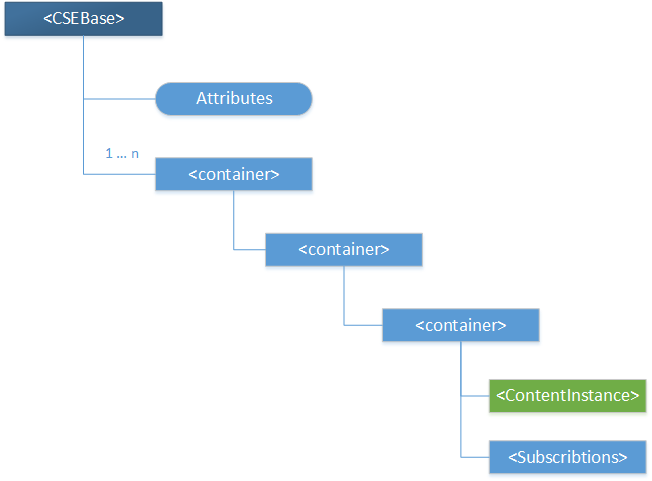
\includegraphics[width=1\textwidth]{resources/images/tree}
    \caption{M2M Resource Tree based on ETSI/oneM2M specifications}\label{fig:contrib1:goal}
\end{figure}
Moreover, since our semantic annotation extension is mainly dealing with sensor data, it adapt the publish/subscribe architecture as well, which facilitate the exchange between sensor networks and cloud-based networks. The publish/subscribe architecture presents a dynamic network pattern to deliver sensor driven processed data to subscriber. It also create a decoupling communication between publisher and subscriber based on time, space and control flow. (Add Request Routing)\par
In most of the cases, those devices and sensors are a non-M2M devices which generate a huge amount of data that need to be semantically annotated and exchanged. To deal with such an issue, the semantic annotation extension consider the interworking proxy entity (IPE) which is a specialized AE defined by oneM2M for interworking with non-oneM2M system as showing in the figure. IPE includes two main functionalities:  
\begin{itemize}
\item translate a non-M2M interface non-oneM2M protocols and massages to oneM2M ones via the Mca interface
\item Mapping non-oneM2M data models into oneM2M resources, which are eventually exposed to oneM2M services.
\end{itemize}\par
Adapting this approach within the core design of our work provide a unique solution that enables communications between different protocols and most importantly, it enables semantic information exchange as well as data sharing [] among the different deployments.


\section{Detailed design model}

\subsection{Overview}
As mentioned in the previous section the design architecture of our work is composed mainly of 4 principle modules. Each module is located in a specific area within the M2M system. The detailed design model of each module is presented in the next subsections.
\sidenote{Intro}


\sidenote{Goal}

\sidenote{Approach}


\subsection{Design and specification of the semantic annotator}

\sidenote{Overview}
The semantic annotator is the most important component of our work as it is responsible for semantically annotating sensors, devices and the type of information they produce (e.g., context of the data, units of the data, type of the data, the location/address, etc.). Hence, the network applications will have the possibility to discover, share and understand the information from different device applications. The main idea of the semantic annotator is to create a child resources for the targeted resources to help represent semantic information. As presented in the previous section, a “resource” is a resource that is addressable using a uniform resource identifier (URI) and stored in the resource repository of a given M2M system, such as the resource tree in oneM2M as shown in the figure (e.g. AE, container, contentlnstance, etc.). In addition, a resource is a uniquely addressable entity in the RESTful oneM2M architecture. It is possible to transfer and manipulate the resource representation by using the four major RESTful methods such as Create, Retrieve, Update, and Delete (CRUD). Moreover, each resource may contain one or more child resources and attributes that store a different set of information about the resources. A child resource is a resource that has a containment relationship with a parent resource. Each child resource is referenced within the representation of its parent resource. Thus, the lifetime of each child resource is limited to its parent’s resource lifetime.\par
Table highlight examples of resources and related child resources defined by TS-0001- OneM2M Functional Architecture version 3. 


\sidenote{Approach}
The M2M architecture provides procedures to discover the different resources available in a specific CSE within a given M2M system. This procedure is knowing as the resource discovery procedure (TS-0018). It is mainly processed using the RETRIEVE method which retrieves the information presented or stored in the resource’s attributes. This can be done by sending a request from a specific originator (e.g. CSE or AE) to a given receiver by including the name of the target attribute in the Content parameter in the request message. When receiving the request, the receiver verifies the presence of the requested resource and checks the originator privileges for retrieving the information related to the resource. The Receiver returns the requested information only if the verification is successfully done. Otherwise, an error is returned instead. Figure TS-0018 present the mentioned procedure for retrieving a given resource.\par
Moreover, as specified in oneM2M-TS-0001 oneM2M Functional Architecture version 3, the usage of the resource discovery procedures can be customized with specified Filter Criteria parameter which limits the scope of the results. To be more specific, the filter criteria parameter provides rules description for resource discovery, (e.g. creation time, resource types, etc.).\par
Using the conventional M2M service layer mechanisms together with the filter criteria can provide effective resource discovery, however, it is not as advanced as we expect for querying resources. Therefore, our semantic annotator’s design consist of providing more advanced mechanisms in order to achieve a more advanced resource query execution. The main design architecture of the semantic annotator aims at realizing semantic-based query by annotating the target resources semantically. In the context of this disclosure, the semantic annotator aims at creating and adding as a child resource the semantic representation of the parent resource. In this manner, all the targeted resources provide a specific semantic representation which allows more advanced query based on semantic.\par
As defined in OneM2M functional Architecture, the type of the resources aiming at providing a semantic representation of target resources which are created by our semantic annotator, is <semanticDescriptor> which will be discussed in more details herein. This type of resources is a crucial component of the semantic annotator design as it allows the storage of the semantic information which principally includes relationship and value information of a given resource in its child resource. Storing the different semantic information in the <semanticDescriptor> resources allows the extraction and the storage of this information in a semantic repository. The semantic repository presented in the next subsection contains mainly a set of triples allowing semantic-based query execution. Also, each semantic annotation instance includes an identifier which is defined by the resource type <semanticDescriptor> associated with some random donation (e.g., a code that may be alphabetic). The main architecture of the semantic annotator instance or the resource type <semanticDescriptor> consist of associating this type of resources with the resources that is included in it's tripled. Thus, each resource type < semanticDescriptor> is mapped to the URIs of the resources of resource repository stored in hierarchical M2M resource structure.  The figure illustrate the M2M Resource Tree that includes the resource type < semanticDescriptor>.\par
\begin{figure}[htbp]
    \centering
    \includegraphics[width=.8\textwidth]{resources/images/resources}
    \caption{M2M Resource Tree based including resource type < semanticDescriptor> }\label{fig:contrib1:goal}
\end{figure}

\sidenote{Integration}
As discussed previously the resource type semantic descriptor is a key of importance for supporting semantic interoperability within an M2M system or M2M service middleware that adapt the oneM2M architecture. This can be done by storing the different semantic descriptions of the targeted resources in its child resources. Within our work, the semantic description is mainly provided by different ontologies which will be discussed in more details in the next subsection. As a result, a targeted resource can have multiple semantic description resources as child resources in case it is semantically described by more than one ontology as showing in the figure bellow.  \par
According to the ETSI/oneM2M specification, each resource in the M2M system includes one or more attribute. This attributes comprises information pertaining to the resource. Moreover, each attribute has a unique name that belongs only to a given resource and value. The resources attribute are uniquely addressable as well. In the table, a set of common attributes of M2M resources is presented.
In the M2M architecture, those attributes are commonly used by all announced resources including the resource type semantic descriptor. Besides the common attributes, there are more specific attributes for the semantic descriptor. Those attributes are shared by all announced < semanticDescriptor > specializations.\par
As specified in oneM2M TS-0004 Service Layer Core Protocol Version 2.7.1, semantic descriptor resource includes five mandatory and optional attributes as showing in the figure.
\begin{figure}[htbp]
    \centering
    \includegraphics[width=1\textwidth]{resources/images/strc}
    \caption{Structure of < semanticDescriptor> resource }\label{fig:contrib1:goal}
\end{figure}
\subsubsection{Mandatory attributes}
Mandatory attributes mean that in case one of this attributes is missing while creating the resource type semantic descriptor, an error would be throwing back, and the creation of the resource is abandoned.
Those attributes are: 

\paragraph*{Descriptor attribute:}

Each semantic descriptor must provide exactly one descriptor attribute. This attribute is responsible for storing the semantic description of the resource whose child resource the <semanticDescriptor> resource is. As mentioned previously, a semantic description is mainly provided by different ontologies within the semantic annotator architecture. More specifically this description shall be according to subject-predicate-object triples as defined in the RDF graph-based data model [4]. The encoding of the RDF triples used in oneM2M is xs:base64Binary as defined in oneM2M TS-0004 Service Layer Core Protocol Version 2.7.1[TS-0004]. Base64Binary is a representation of arbitrary Base64 encoded binary data. To be more specific data in the base64Binary format are encoded using Base64 encoding defined in RFC 4648 [9], which is derived from in RFC 2045 [10].
\paragraph*{RelatedSemantics attribute:}

For creating a new semantic descriptor resource about a resource and potentially subresource within the semantic annotator design, the semantic descriptor resource must contain exactly one related Semantic attribute. As indicated in its name this attribute provide a list of URIs for resources containing related semantic information to the resources where it was created. The URI(s) aims at referencing other <semanticDescriptor> resources. This attribute is importance because it provides means to execute SPARQL queries. This attribute will be presented and explained in more detail in the data access section.
\paragraph*{DescriptorRepresentation attribute:}

Each semantic descriptor must provide exactly one DescriptorRepresentation attribute. This attribute specifies the serialization type of the descriptor attribute. It has a fixed value “application/rdf+xml:1”  which consist of a string composed of a media type followed by an “m2m: encoding” separated by “:” character. 
\subsubsection{Optional attributes}
As defined in oneM2M TS-0004 Service Layer Core Protocol Version 2.7.1[TS-0004], resource of type <semanticDescriptor> can have one or more optional attribute that provide further information depending on the M2M system.
\paragraph*{SemanticOpExec attribute:}
The semanticOpExec attribute contains a SPARQL update request which aims at updating the descriptor attribute. Thus, it is not created or retrieved. 
\paragraph*{OntologyRef attribute:}
 The ontologyRef attribute provide a reference URL of the ontology used to semantically describe the information that is stored in the descriptor attribute. Hence, it is highly recommended to use this attribute in case the information can be described using more than one ontology.\par
The table below summarize all the specific attributes of the semantic descriptor resource.

\begin{landscape}
   \begin{table}[]
\centering
\caption{Attributes of the semantic descriptor resource}
\label{my-label}
\begin{tabular}{llllll}
\hline
\textbf{<SemanticDescriptor> attributes}                              & \textbf{Role}                                                                                                                                                                      & \textbf{Data type}                                                                  & \textbf{Default value}                                                    & \textbf{Mandatory}             & \textbf{Optional}              \\ \hline
\textbf{descriptorRepresentation} & \begin{tabular}[c]{@{}l@{}}specify the serialization \\ type of the descriptor\\ attribute\end{tabular}                                                                   & \begin{tabular}[c]{@{}l@{}}Semantic content \\ representation\end{tabular} & \begin{tabular}[c]{@{}l@{}}application/\\ rdf+xml:1\end{tabular} & \multicolumn{1}{c}{X} &                       \\\midrule
\textbf{semanticOpExec}           & \begin{tabular}[c]{@{}l@{}}Update the descriptor \\ attribute\end{tabular}                                                                                                & SAPRQL                                                                     &                                                                  &                       & \multicolumn{1}{c}{X} \\\midrule
\textbf{descriptor}               & \begin{tabular}[c]{@{}l@{}}Storing the semantic \\ description of the targeted\\ resource\end{tabular}                                                                    & \begin{tabular}[c]{@{}l@{}}base64Binary \\ encoded data\end{tabular}       &                                                                  & \multicolumn{1}{c}{X} &                       \\\midrule
\textbf{ontologyRef}              & \begin{tabular}[c]{@{}l@{}}Provide a reference URL \\ of the ontology used to\\ semantically \\ describe the information \\ in the descriptor attribute\end{tabular}      & URL                                                                        &                                                                  &                       & \multicolumn{1}{c}{X} \\\midrule
\textbf{relatedSemantics}         & \begin{tabular}[c]{@{}l@{}}Provide a list of URIs \\ for resources containing\\ related semantic \\ information to the\\  resources where \\ it was created.\end{tabular} & List of URL                                                                &                                                                  & \multicolumn{1}{c}{X} &                       \\ \hline
\end{tabular}
\end{table}
\end{landscape}
\subsubsection{OneM2M procedures on SemanticDescriptor resource}

As discussed in the last section, each entity in an M2M system that follows the oneM2M architecture is represented as a uniquely addressable resource (e.g. CSE or AE). Thus it is possible to process modify and retrieve resources in oneM2M system. This section specifies the different procedures involved to manipulate information pertaining to a resource of type <semanticDescriptor> and which are located in a standardized resource structure.\par

The information exchange within a procedure is based on the use of Request/Response messages between an originator and a receiver. For example a request/response communication between different CSEs through the Mcc reference point or between AEs and a CSEs through the Mca reference point. The figure illustrates the general flow between an originator and a receiver.\par
\begin{figure}[htbp]
    \centering
    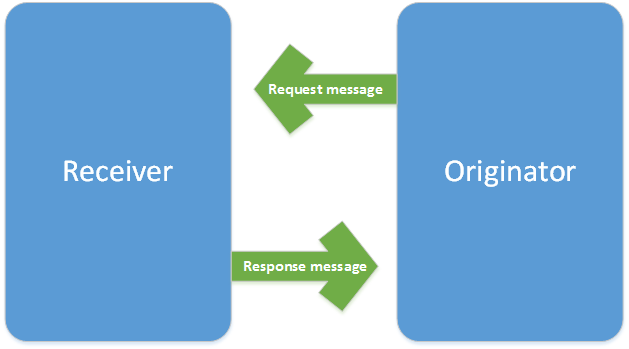
\includegraphics[width=.6\textwidth]{resources/images/response-request}
    \caption{General Flow }\label{fig:contrib1:goal}
\end{figure}
The originator sends a request message over the Mca and Mcc reference points that includes mandatory and optional parameters. The principle mandatory parameter includes mainly the address of the targeted resources, the identifier of the originator and finally the operation to be executed on the resource such as Create, Retrieve, Update, or Delete (CRUD). In case the originator possesses all the privilege to access the resource requested, the receiver send a response message back over the Mca and Mcc reference points. The response message contains mainly mandatory parameters, but it may contain optional parameter as well. The type of parameters returned in the response depends upon the requested operation (CRUD) or the mandatory response code. Therefore, this clause aims at describing the resource type <semanticDescriptor> specific primitive behavior for CRUD operations to communicate efficiently with oneM2M compliant M2M Platform System.\par

\subsubsection*{General resource request procedure for originator }

The Originator shall go through the following action in order to execute a CRUD (in this case a create request) request on a targeted CSE or AE.\par
\begin{figure}[htbp]
    \centering
    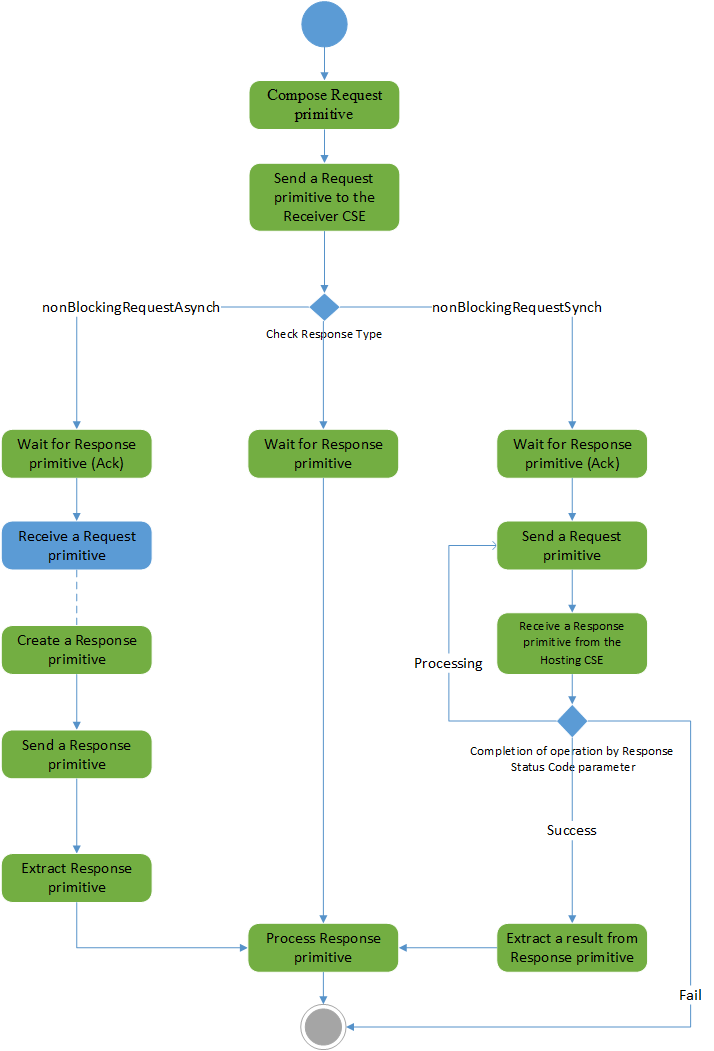
\includegraphics[width=1\textwidth]{resources/images/ori}
    \caption{General procedure of Originator }\label{fig:contrib1:dia}
\end{figure}
As showing in the diagram in Figure~\ref{fig:contrib1:dia}, the first step that should be done by the originator is to compose request primitive message which is mapped to a specific protocol. It is necessary to include in the request message the mandatory parameters previously mentioned such as the operation type, the address of the targeted resources and the identifier of the originator.\par
The second step consists of sending the request message previously composed to the desired CSE. Therefore the originator needs to determine the receiver CSE before sending. 
In the third step, the originator checks if the Response Type parameter is included in the response message. In case it exist, the originator determines the communication method from the Response Type parameter otherwise as specified in oneM2M TS-0004 Service Layer Core Protocol the communication method is set as “blockingRequest” which means that the Receiver CSE responds with the result of the requested operation after finishing processing it. The Response Type parameter includes mainly two different communication method:
\begin{itemize}
\item \textbf{nonBlockingRequestSynch:} based on Onem2M functional architecture, this kind of communication method means that in case the request is accepted by the Receiver CSE, the Receiver CSE responds, after acceptance, with an Acknowledgment confirming that the Receiver CSE will further process the request. As showing in the diagram, several steps follow this Response Type. As specified in the OneM2M functional architecture, within the first step the originator waits for a response from the receiver that corresponds to the sent request. The second step consists of sending a request primitive message from originator to the receiver. The originator must include in the request the mandatory parameters previously mentioned and optionally the optional parameter.  After successfully delivering a request primitive message to the hosting CSE, the originator shall receive mandatory parameters such as the Response Status Code, Request Identifier, and Content. The next following steps depend on form the Response Status Code. If the Response Status Code is successful (e.g. 2000, 2001, 2002, or 2004) and Content parameter exists, the result is extracted from the Response primitive and as a final step the originator process the response. Otherwise, if the Response Status Code is acknowledgment which indicates processing at the Receiver, the originators shall send a new Request primitive message. Finally, in case the Response Status Code is an error (e.g. 4XXX, 5XXX or 6XXX) or the Content parameter does not exist, it moves to finish with an error.
\item \textbf{nonBlockingRequestAsynch:} without going into the details, this method is the same as nonBlockingRequestSynch except that the result of the requested operation is sent back as a notification(s) to the notification target(s).  Therefore, as showing in the diagram, the request procedure compromise additional steps. As specified in the OneM2M functional architecture, within the first step the originator receives Request primitive with mandatory parameters such as operation, Content. In this case, the Operation parameter shall be Notify, and the Content includes notification information related to the originator.  After receiving the Request primitive, the originator shall compose a Response primitive including the mandatory parameters which are Response Status Code and Request Identifier and then send it. After sending the response to the receiver the originator extract the result from the response primitive previously received.
\end{itemize}
\subsubsection*{General request procedure for receiver }

Several steps should be executed by the receiver in a specific order to process a request received from an originator. The receiver shall execute and send an error response in case any error appears in the steps demonstrated in the diagram in Figure~\ref{fig:contrib1:reci}.\par
\begin{figure}[htbp]
    \centering
    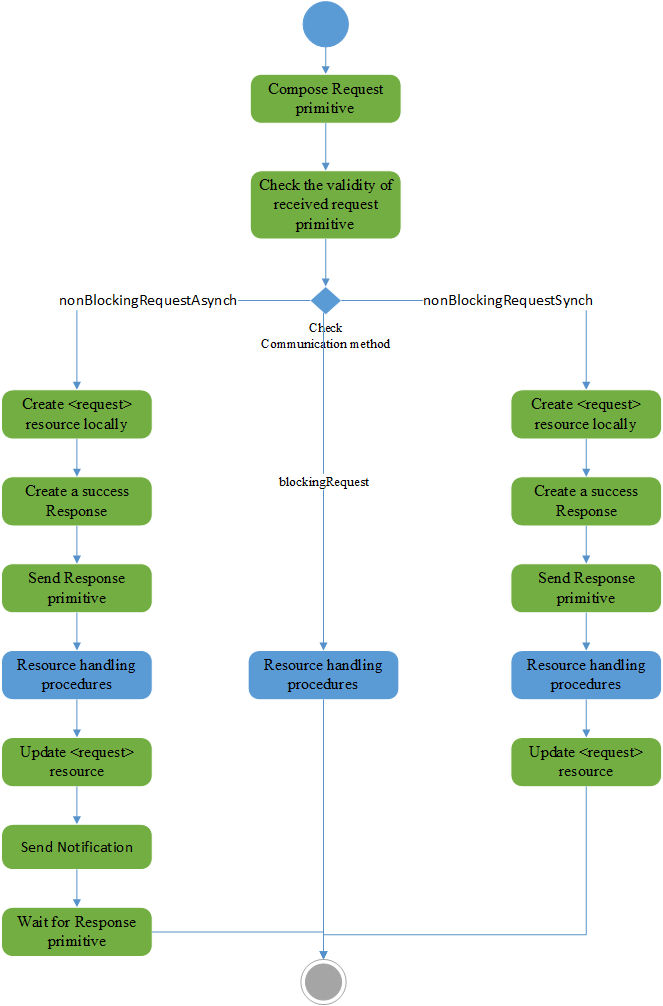
\includegraphics[width=1\textwidth]{resources/images/reci}
    \caption{General procedure of receiver }\label{fig:contrib1:reci}
\end{figure}
Based on the oneM2M specification [ts004], the first step consists of validating the received resource representation against the provided schema definitions.\par
The next step for the receiver CSE is to check the request method received by using Response Type parameter. In case the request is blockingRequest, or the Response Type is not included, it moves to the resource handler procedure step. This step will be discussed in more details herein. Otherwise, if the request is nonBlockingSynch, the receiver CSE shall create <request> resource locally which provide full support for a standardized interface to information representing the context and current status of a request [ts001]. Then the hosting CSE shall create a success response primitive including a response statute code such as CREATED for Create operation, Ok in the case of Retrieve operation, UPDATED for Update operation or DELETED in the case of Delete operation and then send it or forward it back to the originator. After sending the response primitive message, the Receiver goes to the resource handler procedure step which will be presented herein. As a final step, the hosting CSE shall update the <request> resource previously created.
In the case of a nonBlockingAsynch request, the receiver goes through the same steps previously discusses with two extra steps. When the requested operation for a nonBlockingAsynch request is completed, the hosting CSE of the resource shall send a Notify request primitive to inform the final result of requested operation against the oneM2M resource [ts004]. Finally, the originator shall wait for the Response primitive message from the receiver that corresponds to the Request primitive that was previously sent.\par
The receiver goes through a common step in all the different Response type received. The resource handler procedure step. This step calls for extra steps specified for each CRUD operation.
\begin{figure}[htbp]
    \centering
    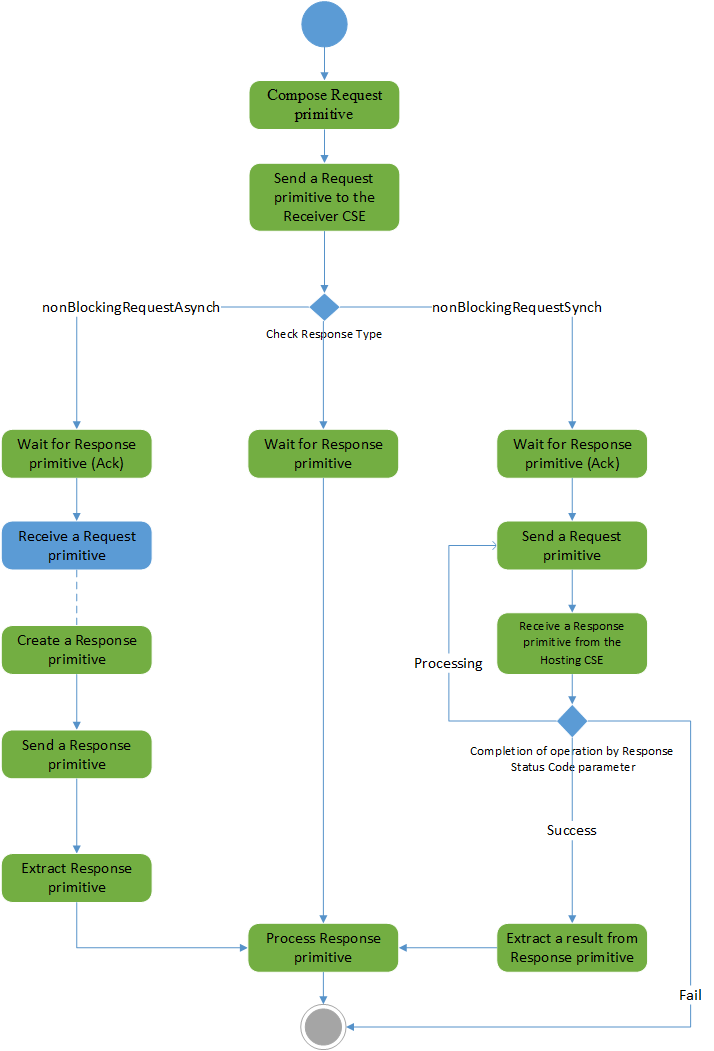
\includegraphics[width=1\textwidth]{resources/images/resource}
    \caption{General procedure of resource handling procedure }\label{fig:contrib1:re}
\end{figure}
 The figure depicts the general procedure to resource handling procedure.\par
The figure bellow describes <semanticDescriptor> resource specific primitive behavior for all CRUD operations for the receiver that specifies the resource handling procedures. \par
The first step is to check whether the receiver is Registrar CSE, the Originator is AE, and operation is created. If the receiver is Registrar CSE and Originator is an AE, the receiver shall check if the sender is allowed to create resource type specified in resource type parameter. Otherwise, check if the receiver is a hosting CSE of the incoming request or a transit CSE. In case the receiver is the hosting CSE, the receiver shall verify the existence of the addressed resources then depending on the target resource type, the Hosting CSE shall check the access control rules of the originator. If there is any rule satisfying all the specific conditions, then the evaluation is successful. Otherwise, it is failed. In the case of success, the receiver shall at first check the validity of resource representation for the CRUD operation requested. For Create and Update CRUD operation there are several extra steps to go through which will be discussed herein.\par
In the case of a valid resource representation, the specific CRUD operation is performed which consist of Creating, Retrieving, Updating or Deleting the resource. The next step consists of announcing the resources in case it contains a specific attribute named “announceTo.” As defined in TS001 an announced resource is a resource at a remote CSE that is linked to the original resource that has been announced, and it maintains some of the characteristics of the original resource. After verifying whether the resource is anounceble or not, the receiver CSE checks the communication method. As mentioned previously in this clause there are three methods of communication. If the request was blockingRequest or Response Type parameter was not included, the receiver composes a success response. Otherwise, it moves to finish. As a final step if the receiver is Hosting CSE, the overall procedure comes to an end by sending the response primitive. In case the receiver is a transit CSE, it needs to execute a Communication Management and Delivery Handling (CMDH) message forwarding procedure only if the Receiver supports the CMDH processing. As defined in ts004, if the Receiver is not compatible with CMDH processing, it shall carry out message forwarding.\item
Depending on the CRUD operation the resource request procedure for the originator and/or the receiver differ slightly from the general procedure previously discussed.\par
\subsubsection*{Create Operation }

For the Create operation, the resource request procedure for the originator keeps the same structure as the general procedure.
In the other hand, when processing the request by the receiver, the descriptor attribute should be a valid RDF/XML syntax. Therefore there are several steps to validate the resource representation before performing the Create Operation. Those specific actions are presented in the diagram in figure \ref{fig:contrib1:create} 
\begin{figure}[htbp]
    \centering
    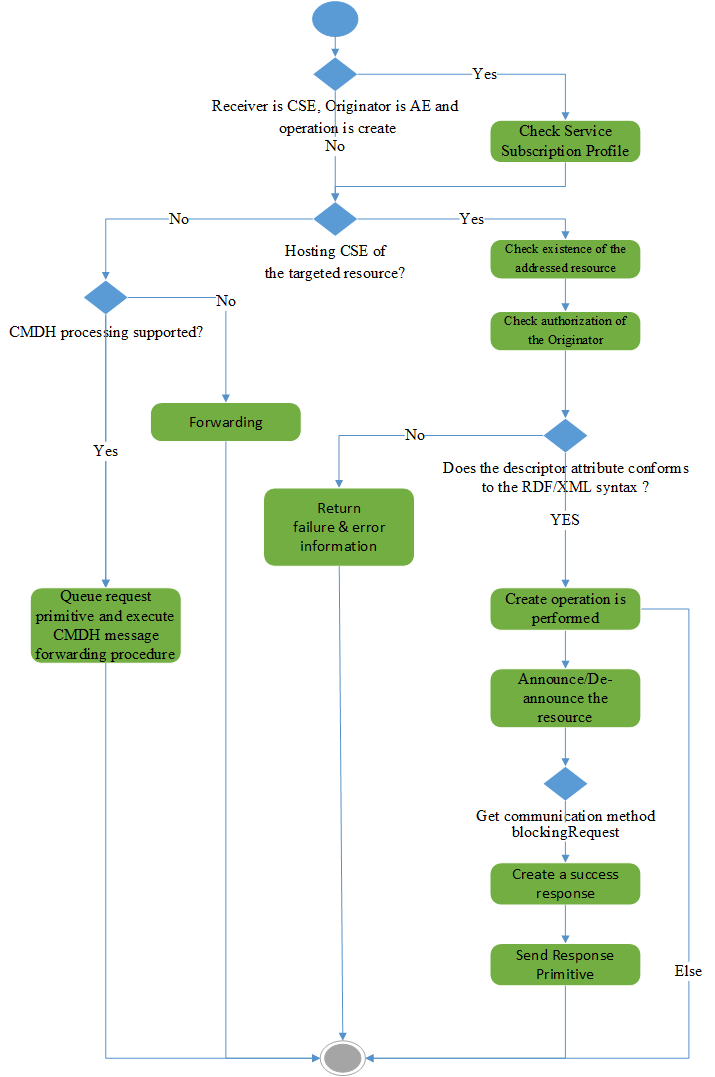
\includegraphics[width=1\textwidth]{resources/images/create}
    \caption{General procedure of Create Operation for the receiver }\label{fig:contrib1:create}
\end{figure}
There is mainly one decision to deal with. In case the descriptor attribute is not a valid RDF/XML syntax as defined in RDF 1.1 XML Syntax, the Hosting CSE return failure, and error information as a response to a CRUD operation format.
\subsubsection*{Retrieve Operation}
The Retrieve operation remains the general resource request procedure for both originator and receiver except that the response message never includes the semanticOpExec attribute.
\subsubsection*{Update Operation}
There is mainly two methods used to update the descriptor attribute:
\begin{itemize}
\item By using the standard method specified in OneM2M architecture to change the descriptor attribute with the new RDF/XML information.
\item By using a SPARQL update by composing a request to update the semanticOpExec attribute in which the value is set to an SPARQL request with SELECT or DELETE statement as specified in the SPARQL query language[]. Thus, the Update operation for the originator keeps the same structure of the general resource request procedure with customizing the "Compose Request primitive" procedure to update the semanticOpExec attribute as mentioned previously.
Concerning the Receiver, when processing the request received, two steps should be modified. 
\end{itemize}
The modification is illustrated in the diagram of the figure \ref{fig:contrib1:update}.
\begin{figure}[htbp]
    \centering
    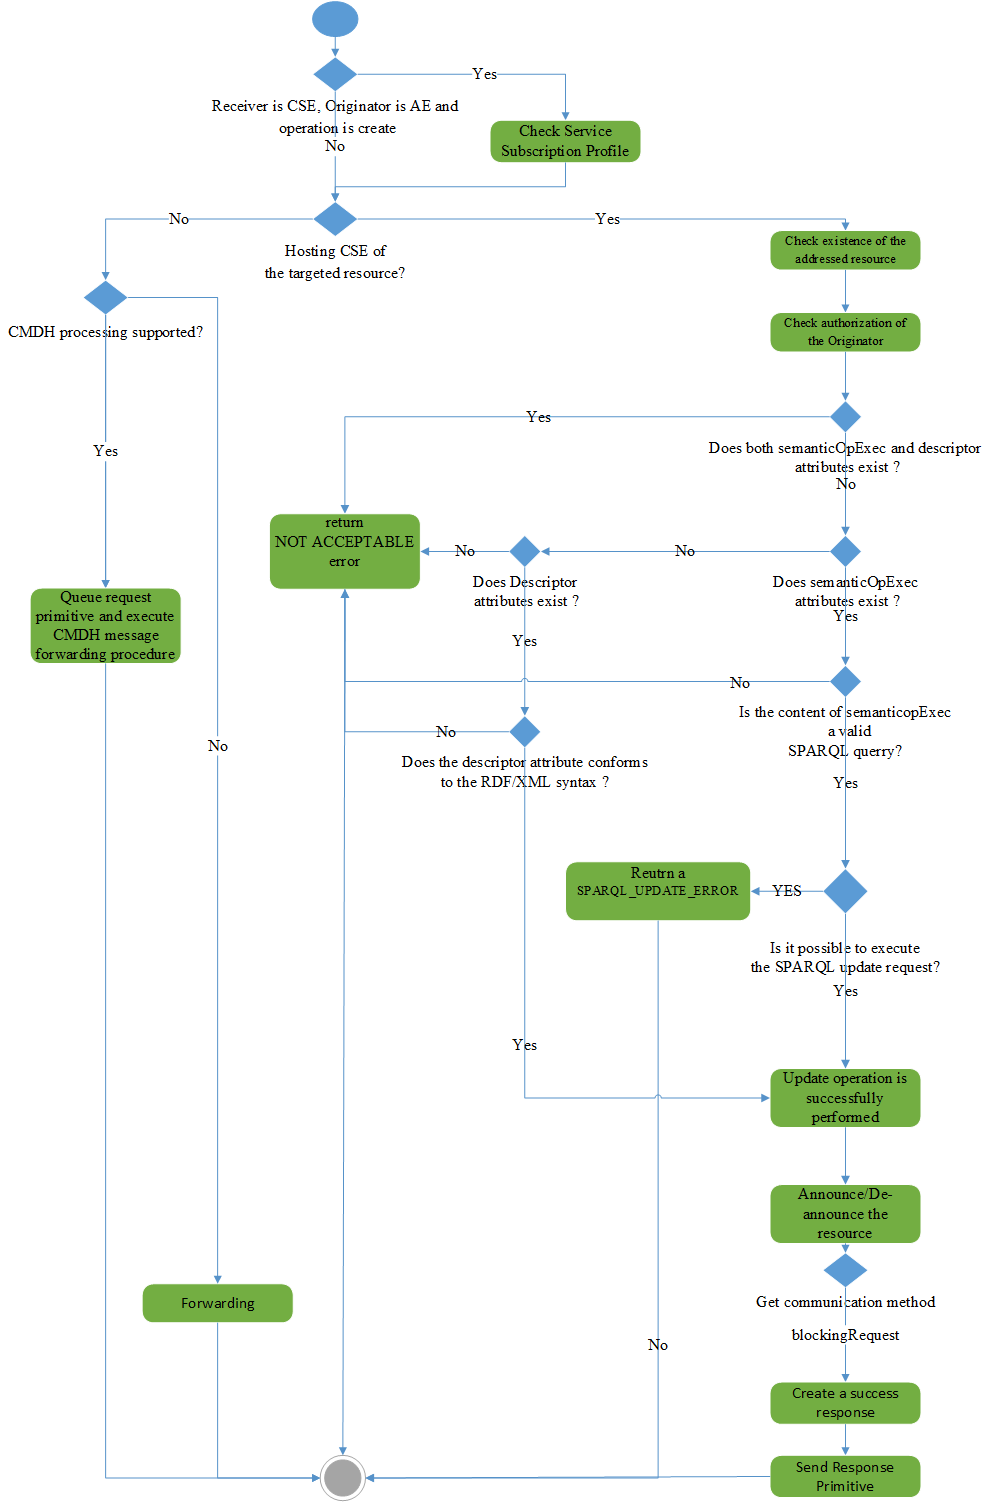
\includegraphics[width=1.1\textwidth]{resources/images/update2}
    \caption{General procedure of Update Operation for the receiver }\label{fig:contrib1:update}
\end{figure}
 First, the "Check validity of resource representation" step need to be modified as follow. The receiver shall check whether both, the semanticOpExec and descriptor attribute exist. If both exist, then the Hosting CSE shall return "NOT\textunderscore ACCEPTABLE" error as specified in OneM2M TS004. Otherwise, if the semanticOpExec only exist, the hosting CSE shall verify if the value of the attribute conforms to a valid SPARQL request. In case it does not conform to a valid SPARQL request, it shall return an "NOT\textunderscore ACCEPTABLE" error. In case the descriptor attribute exist, the receiver shall check if the new information provided conforms to the RDF/XML syntax. Otherwise, it shall return an "NOT\textunderscore ACCEPTABLE" error as well. \item
In the "Update operation is performed" step, if the semanticOpExec attribute exists, the hosting CSE shall execute the SPARQL request. In the case of failure, the receiver shall return "SPARQL\textunderscore UPDATE\textunderscore ERROR" error. Otherwise, it goes to the next step which was previously explained.
\subsubsection*{Delete Operation}
The procedure of Delete operation reminds the same as the general procedure for both originator and receiver.


\subsection{Design and specification of the Semantic Repository}
\subsubsection{Introduction}
\sidenote{Overview}
The preceding subsection described the detailed architecture of the semantic annotator responsible of semantically annotating the content of targeted resources. Thus, the relationship and value information modeled using different ontologies are stored with a resource in its <semanticDescriptor> resources. Due to the fact of the large heterogeneous data annotated and the limited lifetime of some resources, this approach is not completely efficient for Semantic Queries. In fact, Semantic Query is a necessary function in M2M system because it provides full support for resource reasoning, annotation and discovery. This is mainly done by using a Semantic Graph Storages for the Semantic Triples.\par
Therefore, the semantic repository designed for this thesis and presented here provides means to store semantics annotation about all the annotated resources and full support for Semantic Queries. This repository contains mainly a set of triples extracted from all the <semanticDescriptor> resources stored depending on the ontology used for modeling the information within each resource. For example in case there are two different ontologies used to modeled the information and data, the semantic repository will create for each ontology a specific Semantic Graph Store. \sidenote{Approach}\par
In this subsection, we investigate the project design. We will start by positioning the semantic repository regarding the ETSI-compliant M2M platform. Then, we will discuss the different options considered within the architecture for storing the modeled information gathered from various <semanticDescriptor> resources and the motives behind such architecture. Eventually, we will finish by evaluating between all the solutions considered in our work and discussing the architectural option chosen for the design of the semantic repository.
\sidenote{Structure}
\subsubsection{Semantic Repository positioning}
The semantic repository is considered a centralized location in our architecture that aims at managing semantic annotations and provide full support for query languages such as RDF Data Query Language (RDQL), QWL Query Language, SPARQL Protocol and RDF Query Language. It is mainly implemented as part of the M2M system services layer. For example, the semantic repository can be located in a CSE of a given M2M system. The figure below illustrates the positioning of the semantic repository based on the oneM2M high-level architecture.
\sidenote{Positioning}
\subsubsection{Semantic Repository architecture}
Based on the knowledge gained from the overall architecture described in SECTION the semantic repository architecture is inspired from the internal subscription/notification mechanism. In this context, the semantic repository can gather all the information and data needed to be stored. \par
The semantic repository subscribes to the resource of type <semanticDescriptor>. Thus, it grants access to all the attributes available required for accomplishing the Graph Storage. When a new <semanticDescriptor> is available or when modifications to a resource are made, a notification sends by the subscription hosting CSE to the Semantic Repository. Furthermore, the notification scope includes tracking changes of attributes and child resources directly related to the <semanticDescriptor> resource. \par
When receiving a notification from the hosting CSE about a newly created resource of type <semanticDescriptor>, the Semantic Repository shall go through the following actions in the aim of storing the information retrieved. \item
Those actions are described in the figure bellow \par
For each new resource of type <semanticDescriptor>, the Semantic Repository extract the semantic information from the descriptor attribute. In case the data and information are semantically described with more than one ontology, the Semantic Repository check the OntologyRef Attribute to figure the reference URL of the ontology used. Thus, if the ontology used for semantically describing information is not yet stored, the Semantic Repository create a new graph for that specific ontology. Finally the Semantic Repository store or add the concatenate the graph with the graph already stored. Concerning the Graph storage, there are two architectural options considered.
\subsubsection*{First design option}
After extracting the semantic information to be stored from all the <semanticDescriptor> resource available, the Semantic Repository deposes all information gathered, into a local Semantic Graph Store (i.e. Semantic Repository). In this manner, the Semantic repository is implemented as a linked-data databases allowing the management of semantic operations [semantic reference]. \par
This architectural solution provides full support for Semantic Queries with all Semantic Triples available in the Semantic Graph Store. Thus, the Semantic Repository handles the client’s queries (e.g. SPARQL queries) to find the resource semantics information available in the Semantic Graph Store by executing the query in the whole graph and return the results. In case the resource information are modeled with more than one ontology, the Graph Store shall include for each ontology a single graph. Therefore, when processing an SPARQL query, the Semantic Repository shall validate the semantic query operation before executing it. This validation compromises different steps to be followed. First, the Semantic Repository need to check whether the originator has all the privilege to access the resources or not. In the case of access granted, the hosting CSE shall check the OntologyRef attribute in case it is available to decide on which graph the query will be executed. Afterward, the semantic repository conducts the semantic query with the targeted Semantic Graph, and finally, it composes a response to be sent to the originator containing the semantic queries results. \item
The semantic query execution within this solution is illustrated in the sequence diagram in the figure bellow.

 Notwithstanding the above, this solution does not provide full support for semantic discovery and filtering. This is mainly caused by the distributed nature of the <semanticDescriptor> resources. As discussed in SECTION, the key functionalities of the <semanticDescriptor>‘s distributed architecture are enabling semantic filtering. Semantic filtering is a curial component for resource discovery and for specifying the different characteristics of the resource it is interested in. For example, in a normal discovery process, it is possible to filter all the AE resources presenting sensors represented in the M2M system through an IPE and to execute a particular SPARQL query on its \par
  Therefore, this architectural option requires the enablement of the Semantic filtering across the distributed nature of <semanticDescriptor> resources. Hence, there are different solutions considered in this architectural option which is mainly inspired from the under development “TR-0007-Study on Abstraction and Semantics Enablement version 2.9” specification.


\subsection{Conclusion}

\sidenote{Overview}
\todomid{write}

\sidenote{Approach}
\todomid{write}

\sidenote{Integration}
\todomid{write}

\section{Conclusion}

\sidenote{Summary}
\todomid{write}

\sidenote{Takeaway 1}
\todomid{write}

\sidenote{Takeaway 2}
\todomid{write}

\sidenote{Takeaway 3}
\todomid{write}

\sidenote{Next chapter}
\todomid{write}

    \cleardoublepage
\titleformat{\paragraph}
{\normalfont\normalsize\bfseries}{\theparagraph}{1em}{}

\titleformat{\subparagraph}
    {\normalfont\normalsize\bfseries}{\thesubparagraph}{1em}{}
\titlespacing*{\subparagraph}{\parindent}{3.25ex plus 1ex minus .2ex}{.75ex plus .1ex}

\setcounter{secnumdepth}{5}% Display enumeration up to \subparagraph (level 5)
\renewcommand{\theparagraph}{\thesubsubsection.\arabic{paragraph}}
\renewcommand{\thesubparagraph}{\theparagraph.\alph{subparagraph}}

\chapter{Design and Specification}\label{sec:contrib2}\minitoc\vspace{.5cm}
\index{Contribution 2}
\section{Introduction}
This chapter presents the design and specification of the semantic annotation extension introduced in this dissertation. Based on the understanding of the functional and non-functional requirements and the oneM2M architecture presented in the previous chapters, an extension is designed enabling interoperability between things and information within an M2M system complying with the oneM2M specification. As discussed in previous chapters, the current architecture and design of oneM2M system make any M2M Service able to operate in different environments by providing the means to interact with various existing connectivity technologies, such as ZigBee. Interworking with these external technologies makes it possible for the oneM2M application to communicate and interact with diverse heterogeneous devices that are attached to the system. The interworking is based on the Interworking Proxy Entity (IPE), which is defined by oneM2M for interworking with a non-oneM2M system as explained in chapter~\ref{sec:sota}. \par
\begin{figure}[htbp]
    \centering
    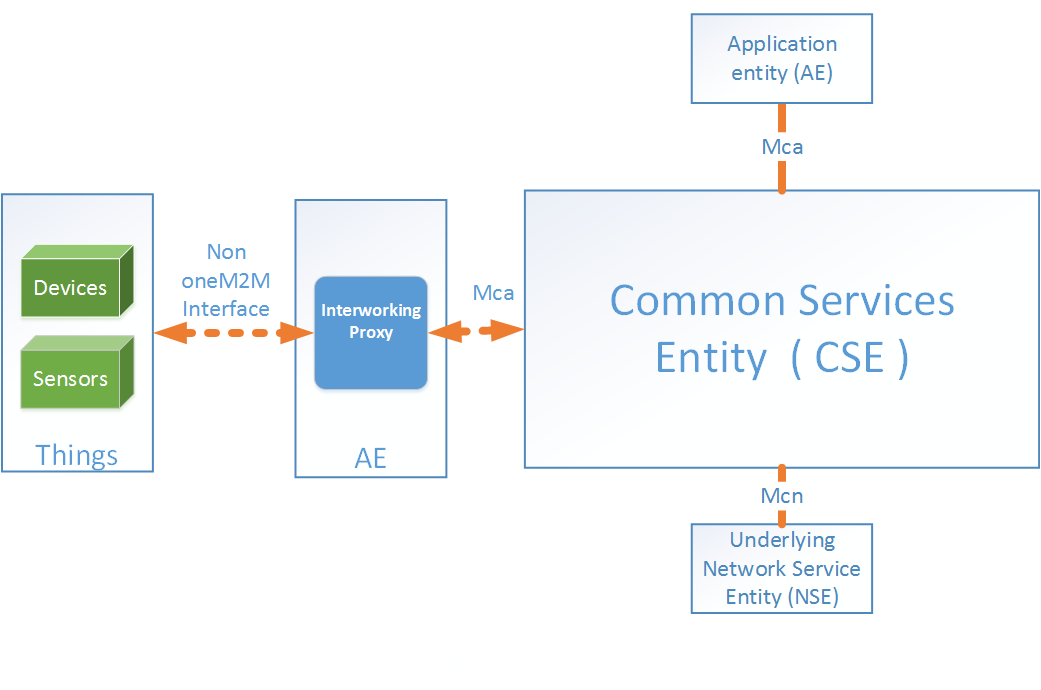
\includegraphics[width=1\textwidth]{resources/images/ini}
    \caption{IPE and oneM2M current architecture}\label{fig:contrib2:cc}
\end{figure}
Although the heterogeneous non-oneM2M enabled devices can be accessed through the Interworking proxy Entity (IPE) to exchange data and information, existing oneM2M implementations and solutions still lack this interoperability feature. Thus, Application needs to understand the semantic and information model of the non-M2M interfaces without going into deep knowledge of the connectivity technologies. For example, within the figure~\ref{fig:contrib2:cc}, the M2M solution presented provides interconnectivity with different devices and sensors through its IPE according to the oneM2M specification. Given two sensors mapped to the system through the IPE within this example. Each sensor includes a specific type. One may have a type "temperature sensor", and the other may have "pressure sensor". Based only on the devices type and their information model, it is not possible to conclude that both of the devices are Sensing Devices. Therefore, the semantic extension design aims mainly at providing additional semantic information to the M2M system by adding references to an ontology such as Fiesta-IoT ontology, that defines "pressure sensor" and "temperature sensor" as a sub-class of "Sensing Device". Such semantic information leverage interoperability between M2M applications. Thus, Applications can directly interact and communicate with real world entities or things through the annotated representation provided by the Semantic Annotation Extension.\par
Constructing an M2M extension that provides semantic interoperability between things can be achieved in various ways. This chapter investigates the Semantic Extension design. First, the Semantic Annotation Extension positioning within an M2M system, is given. Afterward, the Extension architecture and the motives behind such architecture are shown in detail. Eventually, the detailed functions of each module of the Extension and the communication between them are discussed as well.

\section{Extension positioning}
Based on the functional architecture of the oneM2M specification presented in the previous chapter, there are two options where the Semantic Annotation Extension can be located. Either in the Application Entity (AE) or the Common Services Entity (CSE). \par
As illustrated in the figure bellow, the Semantic Annotation Extension should reside inside the CSE. In this manner, the extension can provide communication with different Application Entity using an SPARQL interface as well as Mca reference point interface. On the other hand, this is not easy to handle and to manage in case the Semantic Annotation Extension is located in an Application Entity (AE) because it would be difficult to find the SPARQL interface by other AEs and IoT applications. Besides, locating the Semantic Annotator extension in the CSE facilitate the semantic inter-working with other CSEs via the Mcc reference point. Moreover, since that AEs are supposed to be agnostic towards the existence of other AEs and IPE are a specialized AE, considering locating the Extension inside an AE complicate the communication between the Semantic Annotation Extension and IPEs. Thus, it is more complicated for the Extension not only to describe data and information extracted from different IPEs but also to handle ontologies. Therefore, it is more convenient to reside the Semantic Annotation Extension in the CSE.


\begin{figure}[htbp]
    \centering
    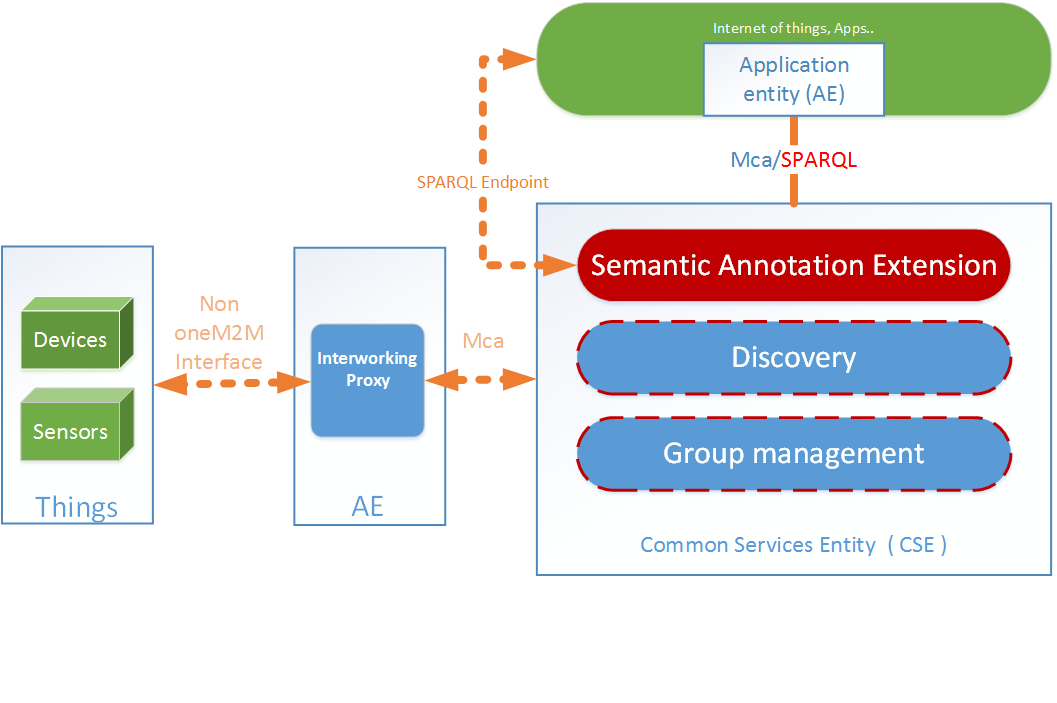
\includegraphics[width=1.\textwidth]{resources/images/positioning}
    \caption{Semantic Annotation Extension positioning in the oneM2M high-level architecture }\label{fig:contrib2:high}
\end{figure}
Going further in adapting the CSE with the semantic functionalities provided by the Semantic Annotation Extension, there are several Common Services Functions (CSFs) that require semantic adaptation by enhancing their functionalities. Those set of CSFs are highlighted in dark red color in figure~\ref{fig:contrib2:high}, such as the data management & repository, discovery and group management CSFs.

\section{Overall Architecture}

As illustrated in figure~\ref{fig:contrib2:2}, the Semantic Annotation Extension architecture focuses on the decomposition of the design into individual components that represent well-defined communication interfaces. Thus, it is composed of two main independent components. Each component includes a set of modules that enable specific functionalities and features. \par
\begin{figure}[htbp]
    \centering
    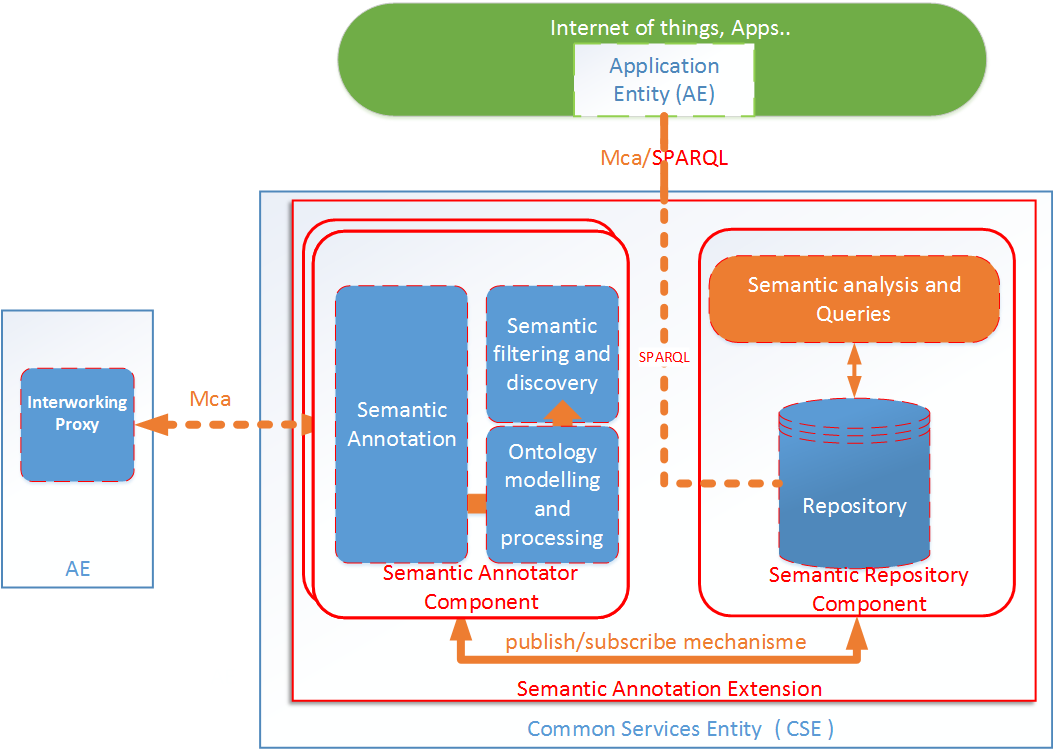
\includegraphics[width=1\textwidth]{resources/images/archi}
    \caption{Functional architecture of the Semantic Annotation Extension }\label{fig:contrib2:2}
\end{figure}
The first component is the semantic annotator which aims at semantically describing information and data extracted from the IPE(s) using a different set of ontologies. It also provides a mechanism for semantic filtering and discovery. Since this component is dealing with data and information extracted from IPE(s), it is required to extend the targeted IPE(s) itself to create a pool of targeted resources. Therefore the IPE within figure~\ref{fig:contrib2:2} is also highlighted in dark red color.\par
The second component is the Semantic Repository which provides means to store semantics annotation pertaining to all the annotated resources and full support for Semantic Queries using SPARQL Endpoint and/or Mca interfaces. \par 
As showing in figure~\ref{fig:contrib2:2}, each component is composed of a different set of coupled modules which offer specific functionalities. The Semantic Annotator component is mainly composed of three different modules:
\begin{itemize}
\item \textbf{Semantic Annotator module} responsible for providing data translation and data interoperability between heterogeneous M2M applications and platform by adding semantic information to M2M resources.
\item \textbf{Ontology modeling and processing module} responsible for linking the resources to different sets of ontology concepts.
\item \textbf{Semantic filtering and discovery module} responsible for extending the M2M discovery mechanism which provides means to link resources and/or services based on their semantic information. 
\end{itemize}\par 

The second component is composed of two main modules:
\begin{itemize}
\item \textbf{Semantic analysis and query module} responsible for enabling query and retrieve operations based on the semantic appliance information of target oneM2M service.
\item \textbf{Semantic Repository module} responsible for storing semantics annotation about all the annotated IPE(s) resources. It contains mainly a set of triples extracted from the annotated resources.
\end{itemize}
Regarding the communication between the two components, it is based on the internal subscription/notification architecture provided by the API of the oneM2M platform which was specified as a communication mechanism of the Semantic Annotation Extension in the previous chapter. This mechanism allows as well the Semantic Annotation Extension to subscribe in a oneM2M system to the targeted resources. This allows the CSE to send back notification as soon as the data is available or updated which enables the extension to manipulate the targeted data and information. \par

\subsection{Design Principles}

The architecture presented here encourages flexibility by its decoupled components, operational reliability and offering higher reusability through the set of modules that defines each component. In this manner, it is possible to manage the semantic operation applied on a given M2M platform. For example, in an M2M platform complying with the oneM2M architecture, each component can be implemented using a dedicated and decoupled plugin. Thus, each plugin can adapt to possible or future changes in its semantic functional requirements (e.g. Semantic Repository is not needed for a specific platform, ontology updating, etc.) or the system requirements (e.g. limited storage space), in a flexible manner without affecting the semantic operation or the performance of the other plugin. Moreover, using a dedicated decoupled component for annotating and semantically describing the resource’s information and data, provide flexibility and effectiveness over the long term as well as the short term. \par
The long-term flexibility and effectiveness are reflected in the ability to use multiple sets of ontologies. Hence, for each ontology, there is a dedicated Semantic Annotator component that can be turned on and off as needed. For the record, within this dissertation, there are two different ontologies used for data and information description and modeling. Therefore, it is mandatory to dedicate within this work for each ontology a particular semantic annotator component. In this context, the semantic annotation extension provides flexibility in adapting ontologies to the M2M platform, simply by adding a new semantic annotator for the desired ontology. Also, dividing each component to a set of modules that provides specific functionalities make it possible as well to adapts the already applied ontologies to the various changes that may occur in the core design of the ontology by only updating the Ontology modeling and processing module.    \par
Concerning the short-term flexibility and effectiveness, it is mainly reflected when the oneM2M platform is modeled using more than one ontology. Then, depending on the implementation method, it is possible to enable/disable the desired ontology simply by activating/deactivating the specific component. Thus, it is possible to use several ontologies to annotate data and information at the same time. \par 

\section{Architecture of Components }
As described in the preceding section, in order to annotate the targeted data and information mapped through the Interworking Proxy entity, it is required to extend the IPE itself which is presented herein. Afterwards, the detailed design and function of the different modules of each component previously presented are given. 
% AEs are supposed to be agnostic towards the existence of other AEs
%SPARQL is not easy to find by all the EAs
\subsection{Extending the Interworking Proxy Entity}
\label{sec:contrib2:ipe}
Based on the knowledge gained from the contexts described in the previous chapter, oneM2M deals with non-oneM2M enabled devices by its IPE(s). IPE is characterized by providing means for mapping the related data model to the oneM2M resources exposed via the Mca reference point~\cite{presentationIPE}. The remapping is mainly done by registering to the hosting CSE at first and then by creating a hierarchical tree resources where the IPE is presented as an <Application Entity> resource. All other relevant data or external information interworked to the oneM2M by the IPE are hosted as children of the <AE> resource. Moreover each resources includes a set of attributes. Those attributes are commonly used by all announced resources. In this manner there are a huge number of resources provided by the IPE(s) depending on the number of devices connected. Some of this resources are relevant to the Semantic annotation Extension and some of them are not. This mainly relay on the ontology used for modeling the resources. Following this approach, the Semantic Annotation Extension is targeting a pool of specific resources. Thus, it is mandatory to extend the IPE in a way to help the Semantic Annotator Extension distinguishing between the resources. \PAR
Extending the IPE to create a pool of targeted resources can be done by defining for each targeted resources a set of labels (keywords)as an attribute. there are a set of labels considered by the Semantic Annotation Extension. Those labels are presented in table~\ref{table:contrib2:label} and ~\ref{table:contrib2:label2}.

\begin{table}[htbp]
\centering
\begin{threeparttable}
\caption{Labels specified for the sensor resources remapped by the IPE}
\label{table:contrib2:label}
\begin{tabular}{lll}
 \hline
\textbf{Sensor resources} & \textbf{Specific Labels}                                                                                      & \textbf{Resource Type}         \\ \hline
Temperature resource      & \textit{\begin{tabular}[c]{@{}l@{}}openmtc:sensor\_data\\ openmtc:sensor\_data:temperature\end{tabular}} & <Container> \\\midrule
Humidity resource         & \textit{\begin{tabular}[c]{@{}l@{}}openmtc:sensor\_data\\ openmtc:sensor\_data:humidity\end{tabular}}    & <Container> \\\midrule
Pressure resource         & \textit{\begin{tabular}[c]{@{}l@{}}openmtc:sensor\_data\\ openmtc:sensor\_data:pressure\end{tabular}}    & <Container>\\\midrule
Movement resource         & \textit{\begin{tabular}[c]{@{}l@{}}openmtc:sensor\_data\\ openmtc:sensor\_data:movement\end{tabular}}    & <Container> \\\midrule
Brightness resource       & \textit{\begin{tabular}[c]{@{}l@{}}openmtc:sensor\_data\\ openmtc:sensor\_data:brightness\end{tabular}}  & <Container> \\ \hline
\end{tabular}
\begin{tablenotes}
      \small
      \item Prefixes can be modified as needed.
    \end{tablenotes}
\end{threeparttable}
\end{table}
\pagebreak

\begin{table}[htbp]
\centering
\begin{threeparttable}
\caption{Labels specified for the device resources remapped by the IPE}
\label{table:contrib2:label2}
\begin{tabular}{lll}
\hline
{\textbf{Device resources}} & {\textbf{Specific Labels}}   & {\textbf{Resource Type}} \\ \hline
ZigBee device resource                          & \textit{\begin{tabular}[c]{@{}l@{}}ZigBee-Device\\ openmtc:device\\ openmtc:device:zig\_bee\end{tabular}} & <Container>\\  \hline           
\end{tabular}
\begin{tablenotes}
      \small
      \item Prefixes can be modified as needed.
    \end{tablenotes}
\end{threeparttable}
\end{table}

\subsection{Design and Functions of the Semantic Annotator}
\sidenote{Overview}
The semantic annotator is the most important component of our work as it is responsible for semantically annotating sensors, devices and the type of information they produce (e.g., context of the data, units of the data, type of the data, the location/address, etc.). Hence, the network applications will have the possibility to discover, share and understand the information from different device applications. As outlined in the previous chapter, the Semantic Annotator component is composed of three coupled modules. The detailed design and function of each module are presented herein.

\subsubsection{Semantic Annotation module}
\sidenote{Overview}
 The main idea of the semantic annotation module is to create a child resources for the targeted resources mapped from an external non-oneM2M technology using IPE to help represent semantic information. As presented in the previous section, a targeted resource is a resource that is mapped to the interworking proxy Entity (IPE), and it includes at least one label as an attribute. The list of the labels handled within the scope of this work is presented in table~\ref{table:contrib2:label} and~\ref{table:contrib2:label2} . Those resources are addressable using a uniform resource identifier (URI) and stored in the resource repository of a given M2M system aligned with the oneM2M specification. In this manner, all the targeted resources provide a specific semantic representation which allows more advanced query based on semantic.\par
 Also, a resource is a uniquely addressable entity in the RESTful oneM2M architecture. It is possible to transfer and manipulate the resource representation by using the four RESTful methods such as Create, Retrieve, Update, and Delete (CRUD). Moreover, each resource may contain one or more child resources and attributes that store a different set of information about the resources. A child resource is a resource that has a containment relationship with a parent resource. Each child resource is referenced within the representation of its parent resource. Thus, the lifetime of each child resource is limited to its parent’s resource lifetime.\par
\sidenote{Approach}
As defined in OneM2M functional Architecture, the type of the resources aiming at providing a semantic representation of target resources which are created by our semantic annotator, is <semanticDescriptor> which was discussed in the previous chapter. This type of resources is a crucial component of the Semantic Annotations design as it allows the storage of the semantic information which principally includes relationship and value information of a given resource in its child resource. Thus, applying this approach provide means to extract and store this information in a semantic repository. The semantic repository presented in the next section contains one graph or more depending on the implementation method. This graph is constructed from the set of triples extracted from the targeted resources allowing semantic-based query execution. Also, each semantic annotation instance includes an identifier which is defined by the resource type <semanticDescriptor> associated with some random donation (e.g., a code that may be alphabetic). As presented in the State of the Art chapter, the oneM2M standard specifies the architecture of the resource type <semanticDescriptor> as an association of this type of resources with the resources that is included in it's tripled. Thus, each resource type <semanticDescriptor> is mapped to the URIs of the resources of resource repository stored in hierarchical oneM2M resource structure.  The figure~\ref{fig:contrib2:example} illustrate an example of the targeted Resource Tree that includes the resource type <semanticDescriptor>.\par
\begin{figure}[htbp]
    \centering
    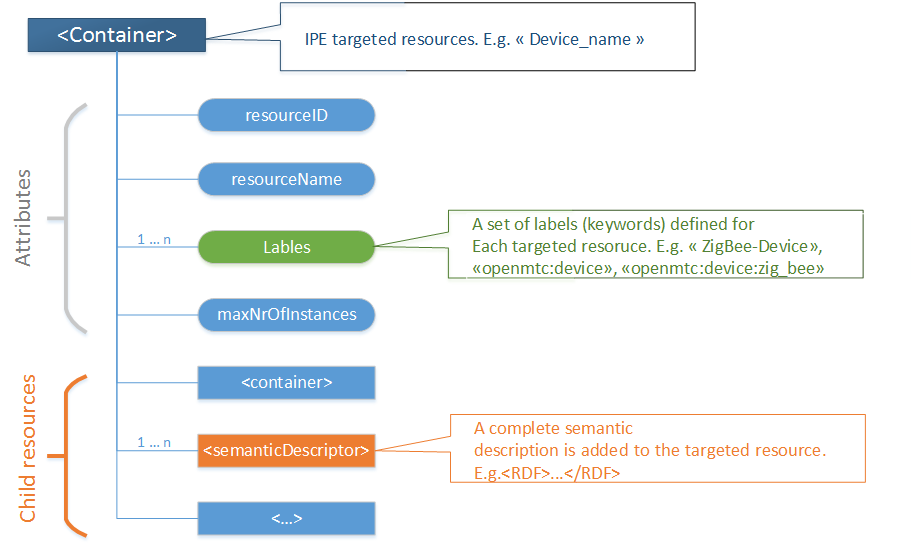
\includegraphics[width=1.1\textwidth]{resources/images/sdlabel}
    \caption{Structure of the semantically annotated targeted resource tree }\label{fig:contrib2:example}
\end{figure}
\sidenote{Integration}
As discussed previously, the resource type semantic descriptor is a key of importance for supporting semantic interoperability within an M2M system or M2M service middleware that adapt the oneM2M architecture. This can be done by storing the different semantic descriptions of the targeted resources in its child resources.
Within our work, the semantic description is mainly annotated by various ontologies which are handled by the Ontology modeling and processing module discussed herein. As a result, a targeted resource can have multiple semantic description resources as child resources in case it is semantically described by more than one ontology.\par
According to the oneM2M specification, each resource in the M2M system includes one or more attribute. This attributes comprises information about the resource. Moreover, each attribute has a unique name that belongs only to a given resource and value. The resources attribute are uniquely addressable as well.
In the M2M architecture, those attributes are commonly used by all announced resources including the resource type semantic descriptor. Besides the common attributes, there are more specific attributes for the semantic descriptor. Those attributes are shared by all announced <semanticDescriptor> specializations. From this perspective, the Semantic Annotation module is responsible for managing the creation of the specific attribute for each <semanticDescriptor> resources. Except for the descriptor attribute which is created by the Ontology modeling and processing module. \par

The semantic annotation module create the <semanticDescriptor> resource for a targeted resource following specific steps. Those steps are illustrated in the sequence diagram bellow~\ref{fig:contrib2:example} .\par
\begin{figure}[htbp]
    \centering
    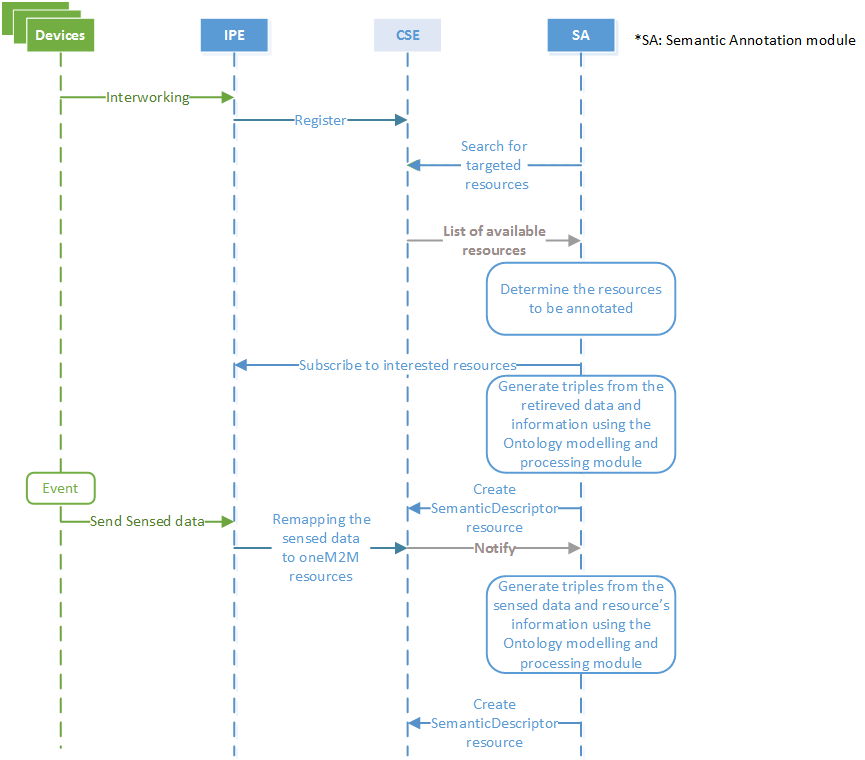
\includegraphics[width=1.2\textwidth]{resources/images/sequence1}
    \caption{Message flow of the <semanticDescriptor> creation }\label{fig:contrib2:sequence1}
\end{figure}
After the registration of the IPE in the hosting CSE and the resource(s) creation procedure is done, the Semantic Annotation module shall determine the IPE resources to be annotated. Therefore, it uses the label attribute as a Filter criteria condition to constrain the scope of tracking. When a targeted label is met, the Semantic Annotation module subscribes to the resource to receive a notification from the Subscription Hosting CSE, each time the attribute(s) or child resource(s) of the subscribed-to resource are modified. After subscribing to the targeted resources, the Semantic Annotation module starts retrieving information and data presented or stored in the resource’s attributes to generate triples and combine them into the descriptor attribute of the <semanticDescriptor> resource pertaining to the retrieved resource. The data and information retrieved depend on the ontology used for modeling which will be further explained in the Ontology modeling and processing module. In case the Semantic Annotation module receives a notification from the Hosting CSE such as a newly sensed data remapped through the IPE as a resource of type <ContentInstance> of the subscribed-to resource, it creates a new resource type <semanticDescriptor> for that <ContentInstance> resource. \par
Since that the Semantic Annotation Extension offer the possibilities to annotate data and information from diverse targeted resources, it may cause problems in case the data are annotated using more than one ontology such as misinterpret the data semantics and types by an application. The problem remains during the execution of a Semantic Query by an originator such as an AE(s) or CSE(s) on the wrong <semanticDescriptor> resource. In other word, the originator may use a particular query that applies to a specific ontology (e.g. Fiesta-IoT ontology),but it will be executed on a different semantic description representation of the same targeted resources which is annotated by a different ontology (e.g. oneM2M base ontology). Thus, there is no guarantee that the hosting CSE which create or update the <semanticDescriptor> resource will always provide the consistent information.\par 
The semantic annotator module is dealing mainly with this problem by providing for each <semanticDescriptor> resource created an ontologyRef attribute which is a reference (URI) of the ontology used to represent the semantic information stored in the descriptor attribute. Thus, it is possible to figure the information provided by the <semanticDescriptor> resource not only by the originator(s) but also by all the several modules and components of the Semantic Annotation Extension. This attribute is necessary for this work, and each <semanticDescriptor> resource must have an ontologyRef as an attribute.




\subsubsection{Ontology modelling and processing module}

One of the challenges of designing the Semantic Annotation Extension is the indexing of the content pertaining to the targeted resources using semantic annotations to provide an explicit knowledge representation. In the purpose of overcoming this challenge, different set of ontologies are considered to annotate the targeted resources because they provide means not only to cleverly structuring a domain but also to use semantic hierarchical and propriety/value relationships based on a vocabulary of concepts~\cite{ontology}.\PAR

The reason behind the usage of multiple ontologies to annotate resource in the core design of the Semantic Annotation Extension is to make it accessible by an extensive and various group of consumers because using only one particular ontology provide interoperability only for users and stakeholder that share and use the same ontology. This design decision is fully supported by the Semantic Annotator Extension as it was explained in the architecture section. In this context, there are a variety of ontologies considered within this thesis.\par
Since that the Semantic Annotation Extension aims at providing the possibilities for the users as well as applications to discover and control sensors and actuators offering specific services and including specific properties in an M2M system, the set of ontologies considered for annotating the data and information shall represent different concepts. Such concepts are deployment system, platform, system, thing, services, devices, sensors, and sensing capabilities, observation, operation unit, kind and their relationships. In a nutshell, the ontology shall be dedicated for IoT platform to help reduce the ambiguity of IoT terminology where resources are mainly related to Sensor, Actuator or devices.\PAR

There are two main ontologies considered within this work. The Fiesta-IoT ontology and OneM2M Base ontology. As discussed in the previous chapter, both of the ontologies fulfill the requirements specified for annotating the targeted resources. Each of the ontology mentioned is explained herein. First, an overview of the different classes, object and data properties considered by the Ontology modeling and processing module is given. Then, the annotation process of the resource is explained.\PAR
\paragraph{Considered elements from Fiesta-IoT Ontology }
\label{sec:contrib2:ele}
In this section, the most relevant Fiesta ontology's classes, object and data proprieties for the Ontology modeling and processing module is presented. The selection process of those elements is mainly based on the scope of the data and information to be annotated. The scope of elements used are presented in Figure~\ref{fig:contrib2:fiesta} and highlighted bellow:
\begin{figure}[htbp]
    \centering
    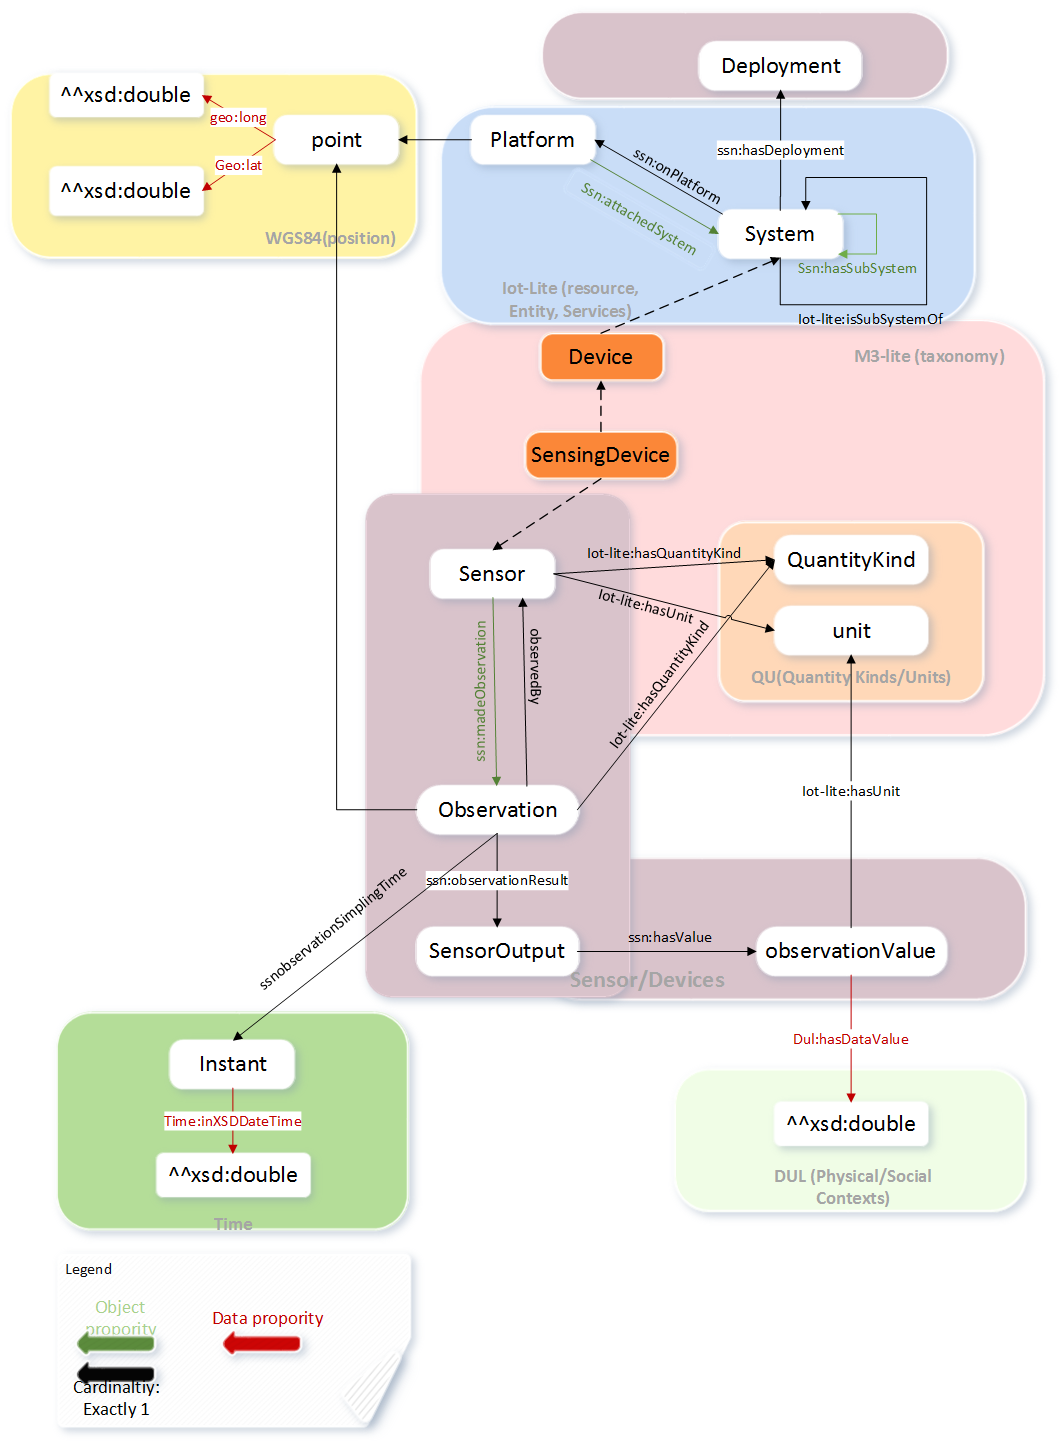
\includegraphics[width=1\textwidth]{resources/images/fiesta}
    \caption{Elements from FIESTA-IoT ontology used by the Ontology modelling and processing module. }\label{fig:contrib2:fiesta}
\end{figure}
\begin{itemize}
\item \textbf{\textit{ssn:Deployment}} presents the root of the graph for every sensor or device in order to identify its owner. For example, a specific Sensor deployed on a Platform or observation campaign.
\item \textbf{\textit{ssn:Platform}} is defined as an Entity that provides the possibilities to other Entities to be attached to it. For example, a device which contains more than a sensor can be defined as a platform.
\item \textbf{\textit{ssn:Device}} is considered by the Ontology modeling and processing module as the core of the resource description. It can be defined as a physical piece of technology - a system in a box. It may as well be built on smaller devices and software components~\cite{device}.Within the scope of Fiesta ontology, these devices are classified as \textit{iot-lite:ActuatingDevice}, \textit{iot-lite:TagDevice} or \textit{iotlite:SensingDevice}. In the scope of this work, the \textit{iotlite:SensingDevice} is considered only. Moreover \textit{ssn:Device} is exposed by an IoT services (\textit{iotlite:Service}). Note that, the IoT services are also in the scope of this thesis.
\item \textbf{\textit{iot-lite:SensingDevice}} can be described as the physical sensors deployed throughout the different M2M systems or Testbeds~\cite{fiesta}. As illustrated in Figure, \textit{iotlite:SensingDevice} is subclass of \textbf{\textit{ssn:Sensor}}. The \textbf{\textit{ssn:Sensor}} class is also relevant for this work because it can be used to describe the variety of devices and sensors remapped thought the IPE and to handle their data gathered from the observations. This \textit{ssn:Sensor} class uses the M3-lite taxonomy~\cite{fiestaiot} such as \textbf{\textit{m3-lite:QuantityKind}} and \textbf{\textit{m3-lite:Units}} to map the physical phenomena that is actually sensed by sensors. Both of those taxonomies are considered in this thesis as well. \textit{m3-lite:QuantityKind} represents sensed phenomenon such as temperature brightness or pressure, as for \textit{m3-lite:Units} it presents a value for a specific thing such as metadata. Since those quantity kinds may be varied depending on the M2M system where it is deployed, it is required to map those quantity kinds to the similar m3-lite quantity kinds. The mapping within this work is presented in table~\ref{table:contrib2:map} bellow. 

\begin{table}[htbp]
\centering
\caption{Mapping of sensors to the convenient m3-lite quantity kinds. }
\label{table:contrib2:map}
\begin{tabular}{ll}
 \hline

\textbf{Sensor}   & \textbf{m3-lite quantity kinds} \\ \midrule
Temperature       & m3-lite\#AirTemperature         \\ \midrule
Humidity          & m3-lite\#Humidity               \\ \midrule
Brightness        & m3-lite\#Illuminance            \\ \midrule
Pressure          & m3-lite\#AtmosphericPressure  \\ \hline
\end{tabular}
\end{table}


\item \textbf{\textit{geo:Point}} is based on the WGS84 ontology~\cite{fiestaiot} and it is responsible of describing the physical location of the devices. The Ontology modelling and processing module uses \textit{geo:lat} and \textit{geo:long} data properties to describe the latitude and longitude.
\end{itemize}
Finally, the Ontology modelling and processing module consider annotating the observations taken by the \textit{SensingDevices} by specifying:
\begin{enumerate}
\item The \textit{m3-lite:QuantityKind} related to the sensor via \textbf{\textit{ssn:observedProperty}}.
\item \textbf{\textit{ssn:observationSamplingTime}} that provides information about the date of the observation by linking it further to \textbf{\textit{Time:Instant}}.
\item \textit{geo:Point } which was previously described.
\item \textbf{\textit{ssn:ObservationValue}} is a subclass of \textbf{\textit{ssn:SensorOutput}} which links to the corresponding value of the observation via the data property \textbf{\textit{dul:hasDataValue}} and \textbf{\textit{m3-lite:Unit}} as showing in Figure.
\end{enumerate}


\paragraph{Annotation process using Fiesta-IoT ontology}

Based on the knowledge gained from analyzing the various elements of the Fiesta-IoT ontology, it is possible to categorize those elements in three main parts: device, sensor, and observation. From this perspective, the annotation process consists of using each part to annotate the equivalent resource. For example, the device part is used to annotate the resource representing a device which was remapped through the IPE. Therefore, the Ontology modeling and processing module shall categorize the resources as well to map each resource to the corresponding part of the ontology. Using this approach, allows the semantic annotation to provide semantic information residing in the Semantic Descriptor resource of the annotated resource that describes only that particular resource according to the Fiesta-IoT ontology.\par
The same concept of the semantic annotation module is used for categorizing the different IPE resources. It is based on filtering the resources remapped through the IPE by its labels. Thus, the Ontology modeling and processing module rely principally on the labels attributes to annotate each resource with its corresponding part of the ontology. As it was mentioned in~\ref{sec:contrib2:ipe}, there are a set of labels that provides information about the resources presented in table~\ref{table:contrib2:label} and ~\ref{table:contrib2:label2}. Each label from the tables~\ref{table:contrib2:label} and ~\ref{table:contrib2:label2}, and its corresponding part of the ontology is presented herein. 
\subparagraph*{Resource with the device labels }
Each resource that includes "ZigBee-Device," "openmtc: device" and "openmtc: device:zig\_bee" as showing in table~\ref{table:contrib2:label2} in its labels attribute shall be annotated with the first part of the ontology illustrated in Figure~\ref{fig:contrib2:fiestadevice} bellow.

\begin{figure}[htbp]
    \centering
    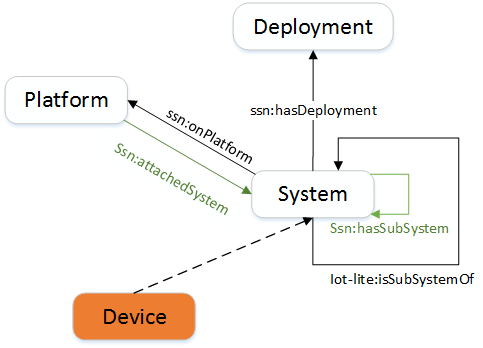
\includegraphics[width=.7\textwidth]{resources/images/device}
    \caption{Annotating the device resources using Fiesta-IoT ontology. }\label{fig:contrib2:fiestadevice}
\end{figure}

Using the different information provided by the device resources such as the \textit{ResourceName} attribute, child resources and parent resources it is possible to create a semantic description corresponding to the resources according to the relevant Fiesta-IoT ontology part illustrated in Figure~\ref{fig:contrib2:fiestadevice}. In case the information is not entirely provided by the resources such as the deployment location, it is always possible to extend the semantic description with the missing information within the Ontology modeling and processing module core depending on the implementation method. Finally, after annotating the resource corresponding to the device remapped through the IPE to oneM2M resources according to the relevant Fiesta-IoT ontology part, the semantic description of the resource shall be elaborated as showing in listing~\ref{lst:contrib3:rw3}. 

\lstset{caption=the semantic description of the resource corresponding to the non-M2M device, label=lst:contrib3:rw3,
language=xml, breaklines=true, numbers=left, basicstyle=\small\ttfamily,
stepnumber=1, frame=single, inputencoding=utf8/latin1}~\lstinputlisting{resources/code/device.rdf}

\subparagraph*{Resource with the sensors labels }
\par 
The same approach used to annotate the resource representing the non-M2M devices is used to annotate the resource representing sensors. The main idea is to annotate each resources containing specific labels in its labels attribute such as "openmtc:sensor\_data:temperature", "openmtc:sensor\_data:pressure", "openmtc:sensor\_data:humidity","openmtc:sensor\_data:brightness" or "openmtc:sensor\_data:movement" as illustrated in table~\ref{table:contrib2:label} by using the sensor part from the Fiesta-IoT ontology specified previously and illustrated in Figure~\ref{fig:contrib2:fiestasensor} bellow. 

\begin{figure}[htbp]
    \centering
    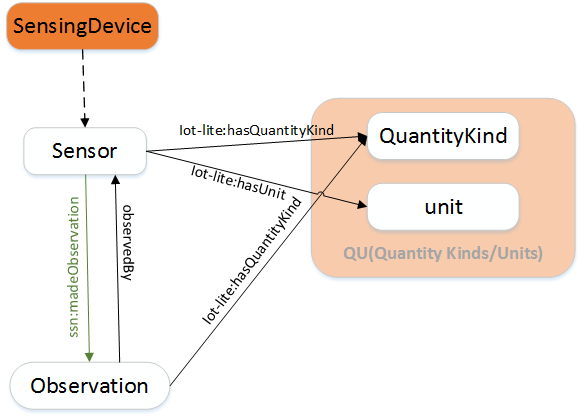
\includegraphics[width=.7\textwidth]{resources/images/sensor}
    \caption{Annotating the sensors resources using Fiesta-IoT ontology. }\label{fig:contrib2:fiestasensor}
\end{figure}

After annotating the resource corresponding to the device which was remapped through the IPE to oneM2M resources according to the relevant Fiesta-IoT ontology part using the different information retrieved from the targeted resource, the semantic description of the resource shall be elaborated depending on the sensor type. listing~\ref{lst:contrib3:rw4} shows the semantic description of a temperature sensor.

\lstset{caption=the semantic description of the resource corresponding to a sensor, label=lst:contrib3:rw4,
language=xml, breaklines=true, numbers=left, basicstyle=\small\ttfamily,
stepnumber=1, frame=single, inputencoding=utf8/latin1}~\lstinputlisting{resources/code/sensor.rdf}


\begin{figure}[htbp]
    \centering
    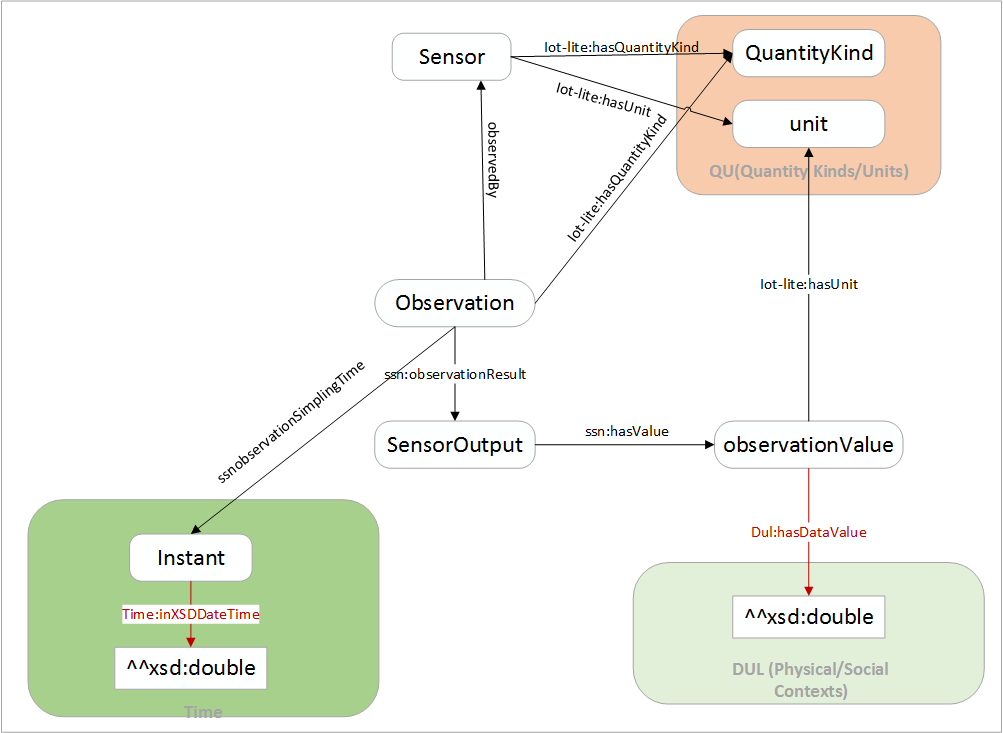
\includegraphics[width=.9\textwidth]{resources/images/ci}
    \caption{Annotating the sensors data using Fiesta-IoT ontology. }\label{fig:contrib2:ci}
\end{figure}

Since that the IPE push the sensor data aggregated from those sensors to a child resources type content Instance of the corresponding sensor resource, the Ontology modeling, and processing module is supposed to annotate the data residing under the content Instance resource as well. In other words, each content Instance resource residing under a resource presenting a sensor and including one of the labels mentioned in table ~\ref{table:contrib2:label} should be semantically annotated in a dedicated instance and not in the same instance of the parent resource. For example, if a container corresponding to a sensor which includes \textit{"openmtc:sensor\_data:humidity"} as a label in its label attribute, has more than one content instance, all of its content instances should be semantically annotated depending on their contents. In this context, each content instance has its respective semantic Descriptor as a child resource.\par
 

In case a content instance meet all the condition previously explained, the observation part from the Fiesta-IoT ontology illustrated in Figure~\ref{fig:contrib2:ci} shall be used to create a semantic description for all the information residing in its \textit{content} attribute. Also, as explained in~\ref{sec:contrib2:ele} each quantity kind provided by the Content attribute of the content instance resource should be mapped to the equivalent m3-lite quantity kind as illustrated in Table~\ref{table:contrib2:map}.\par

From this perspective, depending on the sensor type (temperature, humidity\ldots) the descriptor of the Semantic Descriptor attribute for each content Instance resource shall provide a semantic description that follows the observation part derived from the Fiesta-IoT ontology. For example, the semantic description of a content Instance pertaining to a temperature sensor is illustrated in~\ref{lst:contrib3:rw5}.\par

\lstset{caption=the semantic description of the resource corresponding to a content instance, label=lst:contrib3:rw5,
language=xml, breaklines=true, numbers=left, basicstyle=\small\ttfamily,
stepnumber=1, frame=single, inputencoding=utf8/latin1}~\lstinputlisting{resources/code/content.rdf}

\paragraph{OneM2M Base Ontology }
\paragraph{Semantic Query support }
\label{sec:contrib2:onq}
The distributed and independent manner of the semantic representation provided by the Ontology modeling and processing module aims at enabling resource discovery using semantic as well as semantic Query. Notwithstanding the previous sentence, providing semantic Query in a collection of an independent semantic description located independently in different semantic descriptor resources is problematic. In the context of this work, the Semantic Annotator Extension faces this problem directly by its Semantic filtering and discovery module and indirectly by the Ontology modeling and processing module. \par
Since that all the information and data semantically annotated by the Ontology modeling and processing module are related, their semantic representation should be linked as well. To be more specific, the semantic description pertaining to the targeted resources and located in the Semantic Descriptors should form a whole complete graph when they are gathered together for query proposes. \par
For this reason, there are several solutions considered within the Ontology modeling and processing module. The first solution consists of using a blank node (also called bnode) which is an RDF node but does not contain any data or information~\cite{bnode}. It is mainly for grouping different set of data that can have a common parent node. From an RDF/XML syntactical standpoint, a bnode is rdf:Description element that is not assigned to an rdf:about. Using this solution require more specification because merging a set of semantic description that includes the same bnodes in the same graph makes the identification of this bnodes in the combined graph impossible and they will be identified as a unique bnodes and not related~\cite{w3crdf}. Therefore, it is necessary as specified in~\cite{bnode}, to provide a blank node identifier for identifying each bnode, such as the sensor and its observations where the bnode links the sensor and its corresponding observations. \par
The second solution uses the same concept as the previous solution, but instead of using a blank node identifier, the Ontology modeling and processing module uses an additional URL to link between two semantic descriptions. There are several ideas to define the URL. This URL can be for example the URL of a <semanticDescriptor> resource, where additional RDF triples for the given class instance can be found, or it can be a newly defined URL associated with some random donation (e.g., a code that may be numeric which illustrate the number of the observation made by the sensor). We do not have to choose between the two solutions as they both provides the same results and it highly dependent on the implementation preferences. 

\subsubsection{Semantic filtering and discovery module}
\sidenote{Overview}
The oneM2M architecture provides procedures to discover the different resources available in a particular CSE within a given M2M system. This procedure is knowing as the resource discovery procedure~\cite{TS}. It is mainly processed using the RETRIEVE method which retrieves the information presented or stored in the resource’s attributes. This can be done by sending a request from a specific originator (e.g. CSE or AE) to a given receiver by including the name of the target attribute in the Content parameter in the request message. When receiving the request, the receiver verifies the presence of the requested resource and checks the originator privileges for retrieving the information related to the resource. The Receiver returns the requested information only if the verification is successfully done. Otherwise, an error is returned instead. 
Moreover, as specified in oneM2M-TS-0001 oneM2M Functional Architecture version 3, the usage of the resource discovery procedures can be customized with specified Filter Criteria parameter which limits the scope of the results. To be more specific, the filter criteria parameter provides rules description for resource discovery, (e.g. creation time, resource types, etc.).\par
\sidenote{approach}
Using the conventional oneM2M service layer mechanisms together with the filter criteria can provide efficient resource discovery. However, it is not as advanced as we expect for querying resources. Therefore, our semantic annotator’s design consists of providing through its Semantic filtering and discovery module more sophisticated mechanisms in order to achieve a more advanced resource query execution. The main design architecture of the Semantic filtering and discovery module aims at enabling semantic filter criteria. Semantic filter criteria are defined in the oneM2M specification Study on Abstraction and Semantics Enablement version 2.11~\cite{211} , as the semantic description presented in one of <semanticDescriptor> child resources that match the specified semantic filter. Thus, it can be specified as the possibilities to execute SPARQL requests on each semantic descriptors of the targeted resources. From this perspective, the overall result for the semantics filter criteria is true if one or more of the semantic filters matches the semantic description. The following two examples demonstrate the semantic filter criteria within the current Semantic Extension architecture by executing two different SPARQL queries on two semantic descriptions. The first semantic description pertains to a temperature sensor and the second pertains to its content instance. For the sake of facilitating understanding, the two annotations illustrated in~\ref{lst:contrib3:rw5} and~\ref{lst:contrib3:rw5} are used to execute the queries.  \par 

Since that the semantic description of the targeted resource in~\ref{lst:contrib3:rw5} and~\ref{lst:contrib3:rw5} is annotated using Fiesta-IoT ontology, the SPARQL request should be as follow. 

 \lstset{caption=First SPARQL query, label=lst:contrib3:s1,
language=xml, breaklines=true, numbers=left, basicstyle=\small\ttfamily,
stepnumber=1, frame=single, inputencoding=utf8/latin1}~\lstinputlisting{resources/code/sparql1.java}

The results of the previous SPARQL request on the content of the semantic descriptor representing temperature sensor is \textit{Device\_resource}. In the other hand, the results of the content of the semantic descriptor representing pressure sensor is empty which make sense because it does not includes the the requested information. \par 
\sidenote{Problem with this approach}
the second example consist of executing the SPARQL request as showing in~\ref{lst:contrib3:s2} on the content of the semantic descriptor of temperature sensor.

 \lstset{caption=Second SPARQL query, label=lst:contrib3:s2,
language=xml, breaklines=true, numbers=left, basicstyle=\small\ttfamily,
stepnumber=1, frame=single, inputencoding=utf8/latin1}~\lstinputlisting{resources/code/sparql2.java}

Although the temperature sensor provides a set of temperature values through its content instance resources which are annotated as well according to the functional architecture of the semantic annotation module as showing in~\ref{lst:contrib3:s2}, the results of the SPARQL query is empty. This can be explained by the fact that the relevant semantic information requested which is, in this case, the temperature value is not contained in the <semanticDescriptor> child resource of the temperature sensor resource directly but in its <contentInstance>'s <semanticDescriptor> resource.\par 

The overall goal of the Semantic filtering and discovery module is to provide a solution for the problem explained in the second example which consist of affording semantic filtering on the distributed Semantic Descriptors. As it was described previously in~\ref{sec:contrib2:onq}, this problem is already handled at the annotation level by the Ontology modeling and processing module. In the other hand, this issue is solved at the resource level by the Semantic filtering and discovery module. The main idea of this module is to link all the different <semanticDescriptor>(s) in case a semantic filtering or any other semantic operation is applied to the complete semantic graph or part of it. The general idea is demonstrated in Figures~\ref{fig:contrib2:dg}. \par 
The case of the semantic filter of the second SPARQL query whose scope takes into account semantic information stored in different <semanticDescriptor> resources is illustrated inFigure~\ref{fig:contrib2:scope}. The <semanticDescriptor> resource describing the sensor and the <semanticDescriptor> resources describing its <contentInstance>.
\begin{figure}[htbp]
    \centering
    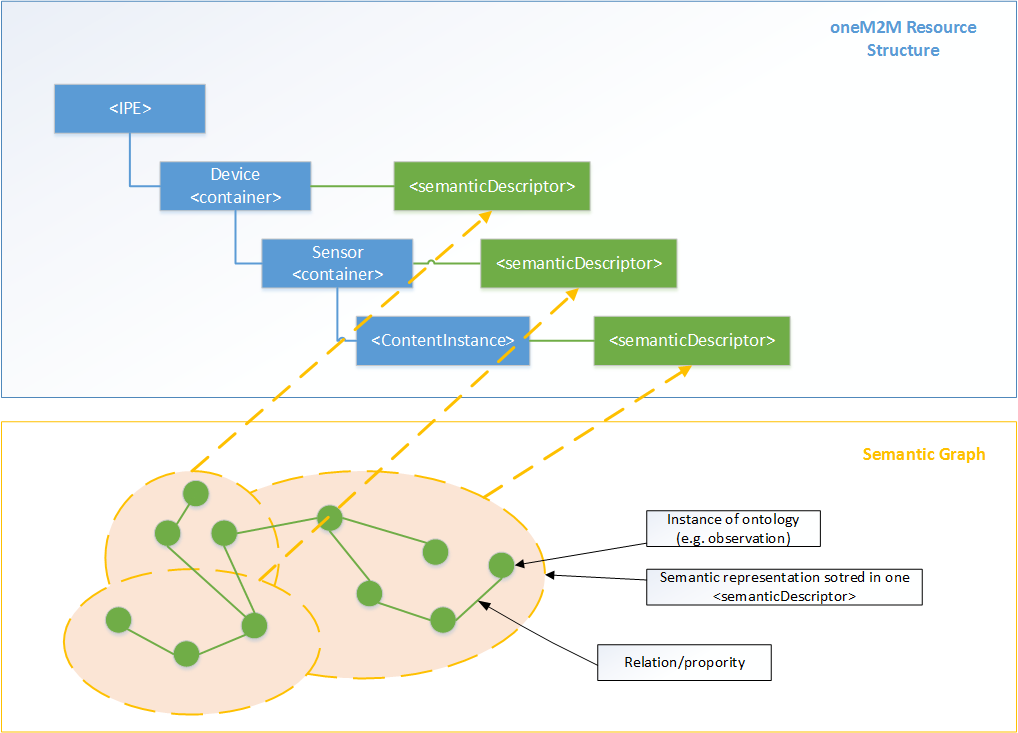
\includegraphics[width=1.\textwidth]{resources/images/dg}
    \caption{Mapping of logical semantic graph to oneM2M resource structure inspired from~\cite{211}. }\label{fig:contrib2:dg}
\end{figure}

\begin{figure}[H]
    \centering
    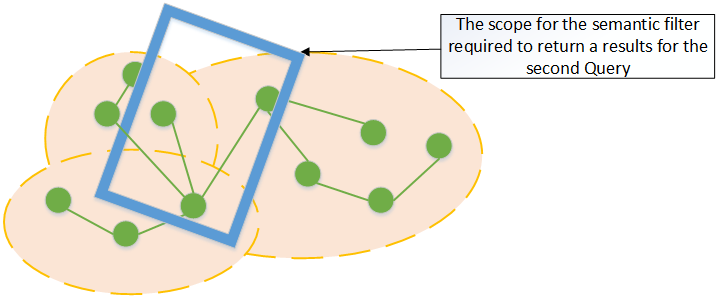
\includegraphics[width=1\textwidth]{resources/images/scope}
    \caption{Scope of semantic filter across semantic information stored in different resources inspired from~\cite{211}. }\label{fig:contrib2:scope}
\end{figure}

%\sidenote{Considered Solutions}
Before explaining the solution considered in this work to solve the semantic filter criteria on the distributed semantic descriptor problem, the several solutions available are discussed and compared herein to demonstrate the reasons behind such a choice for the solution.
 
\paragraph{First solution: }
\sidenote{First solution }
The concept of this solution is similar to the solution applied in the Ontology modeling and processing module to handle the distributed manner of the semantic representation which was already explained in~\ref{sec:contrib2:onq}. In this manner, the Semantic filtering and discovery module uses a resourceDescriptorLink which is an OWL annotation property defined in~\cite{211}. As it was explained in~\ref{sec:contrib2:onq}, this annotation propriety consist of using the URL of a <semanticDescriptor> resource which contains the information related to the <semanticDescriptor> resource included in a semantic filtering operation. For example, applying a specific filter request for sensors that produce temperature output which has the SPARQL query representation showing in~\ref{lst:contrib3:s2}, require the usage of the two semantic descriptions of the temperature sensor and its <contentInstance> illustrated in~\ref{lst:contrib3:g1} and~\ref{lst:contrib3:g2}. From an ontology annotation point of view, as demonstrated in Figure~\ref{fig:contrib2:link}, the output of the temperature sensor requested is described as an observation based on Fiesta-IoT ontology. Therefore the observation in the semantic description of the temperature sensor should be linked to the observation in the semantic description of the <contentInstance>. From this perspective, the resourceDescriptorLink aims at linking the observation of the semantic descriptor resource of the candidate resource where the SPARQL request is executed, with the observation of the semantic descriptor resource related to it. Thus, each time during the SPARQL request execution a class instance is encountered with a resourceDescriptorLink annotations, the content of each of the <semanticDescriptor> resources the resourceDescriptorLink references should be added to the content on which the SPARQL request is being executed to form a larger content. Then the SPARQL execution continues on the enlarged content. 

\begin{figure}[htbp]
    \centering
    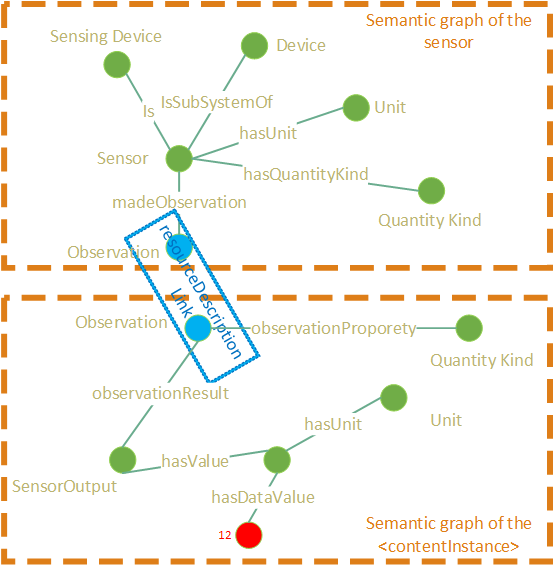
\includegraphics[width=.7\textwidth]{resources/images/link}
    \caption{Semantic filter for sensor that produce temperature output. }\label{fig:contrib2:link}
\end{figure}

\paragraph{Second solution}
In contract to the previous solution, this solution provides semantic filtering on the distributed Semantic Descriptors at the resource level instead of the semantic description level. It consists of providing an additional attribute for indicating all the resources with resources related to the candidate resource. This attribute is defined by the oneM2M specification as the relatedSemantics attribute. From this perspective, when performing a semantic filtering operation, it is required to fetish all the links available in the relatedSemantics attribute of the candidate resource and to retrieve the corresponding semantic descriptions from the descriptor attribute. Afterward, all those sub-graphs retrieved shall be merged in order to create a complete graph. As a final step, the SPARQL request representing the semantic filter operation will be executed across the resultant enlarged graph. As illustrated in the Figure~\ref{fig:contrib2:rs}, applying this approach to the semantic description of the temperature sensor resource, require the creation of a list containing all the related resources to the semantic description temperature sensor resource. In this case, this list should include the path of the semantic description presenting the device of the sensor and the semantic description of the output provided by the sensor which is in a normal case pushed to the <contentInstance> resource of the sensor resource. This list previously defined should be fetched each time a Semantic Query is performed on the semantic description of the temperature sensor resource to create a larger resultant graph which includes all the semantic description related to a temperature sensor.

\begin{figure}[htbp]
    \centering
    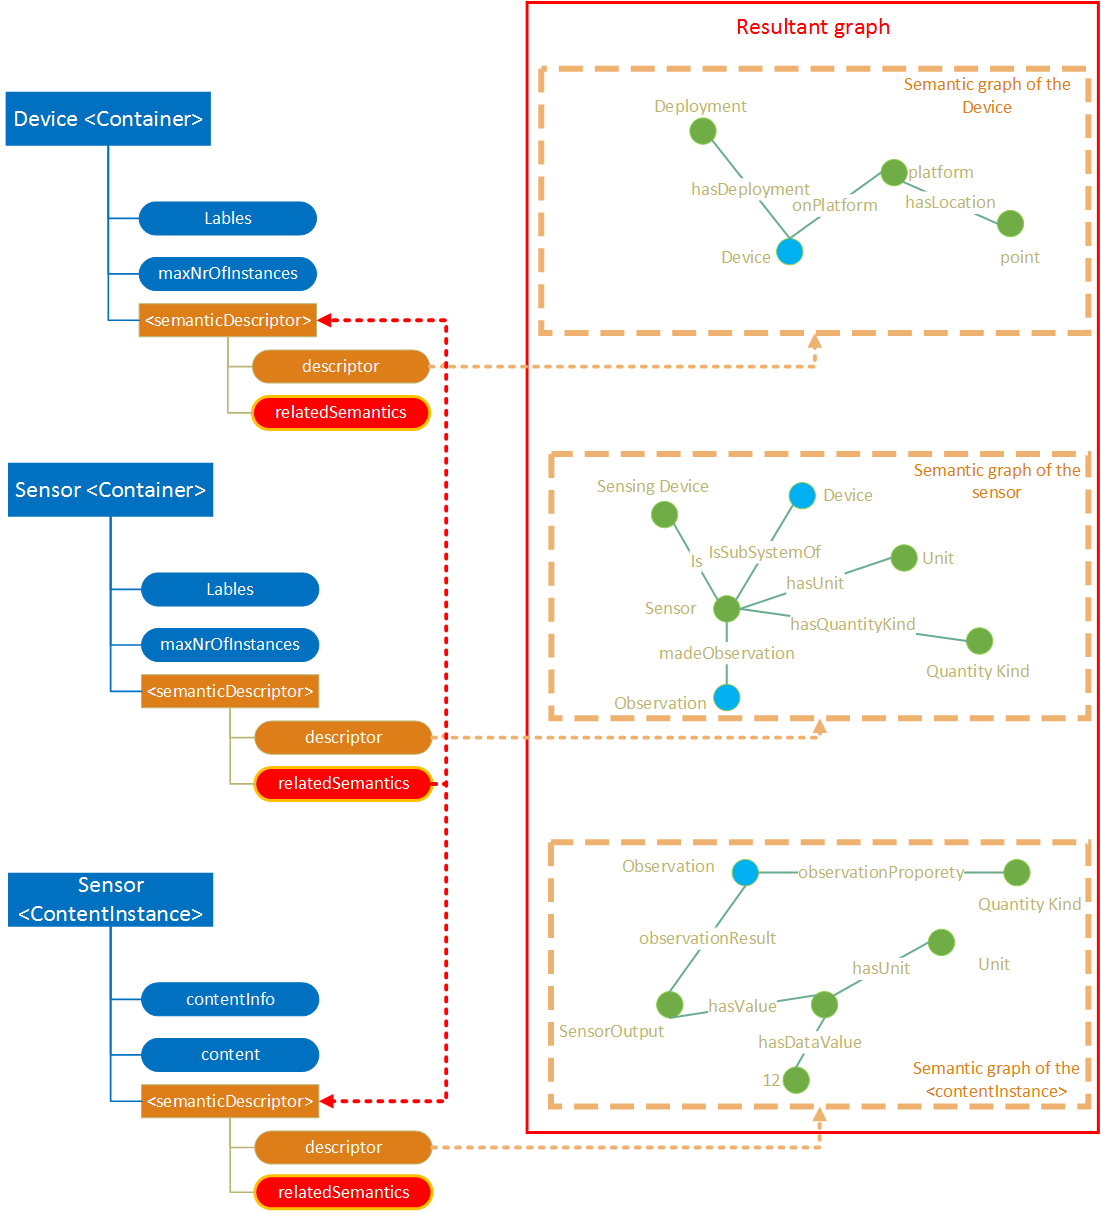
\includegraphics[width=1\textwidth,left]{resources/images/rs}
    \caption{Use of relatedSemantics attribute. }\label{fig:contrib2:rs}
\end{figure}

\paragraph{Comparison between the two solutions}
In order to select the appropriate solution, this section provides the comparison between the two solution presented previously.\par 
Both of the solutions presents semantic filtering on the distributed Semantic Descriptors by providing means to find the required semantic information. They also provide resource-based access control by enabling access to the semantic information at execution time of the operation. \par 
The main difference between both of the solutions is that the first solution requires the modification of the SPARQL request each time a new resourceDescriptorLink is encountered. This is caused by the fact that the SPARQL request needs to retrieve the semantic description linked by the resourceDescriptorLink to retrieve the semantic information required. In the other hand, the second solution does not require the modification of the SPARQL request during the execution which can be classified as an advantage of using this solution. Another advantage of the second solution is reflected in the ability to link more than one concept in different descriptors attribute by only one link which avoids the duplication of content being considered for processing the SPARQL request. \par 
The only disadvantage of the second solution compared to the first one is that each time an SPARQL request is executed all the links located in the \textit{RelatedSemantic} attribute has to be fetched even if it is not required to submit the SPARQL query. Thus, it may cause a problem in case the \textit{RelatedSemantic} attribute includes a huge list of related <semanticDescriptor> resources. In contrast, the first solution by its concept avoid this issue because the SPARQL query has to be aware of the directly related instance in other <semanticDescriptor> resources, but it still needs to modify the SPARQL query each time as it was explained previously.\par


\paragraph{Specific Design Decisions}

Based on the understanding of the difference between the two solutions and analyzing their strength and weakness. The second solutions are adapted within the core design of the Semantic filtering and discovery module. This solution was chosen over the first one for a particular reason. The fact that the second solution does not require the modification of the SPARQL query during the execution time is a significant advantage. Thus, the applications or CSE(s) execute a query which will be directly executed on the resultant enlarged graph derived from the links in the \textit{RelatedSemantic} attribute. But as explained previously, one may say that this solution is problematic in case the \textit{RelatedSemantic} attribute contain a huge list of links. In fact, this can be true on a large scale of data to be annotated which is not the case of this work because the semantic annotation is targeting only a set of specific resources that includes well-defined labels. Thus, using the labels attribute of each annotated resource can help in defining the relations between the different <semanticDescriptor> resources. Moreover, it is possible to limit the number of links in the \textit{RelatedSemantic} attribute in case it includes the different set of related <semanticDescriptor> resources pertaining to <contentInstance> which may lead to overload the \textit{RelatedSemantic} attribute because they are created based on events. The limitation can be done based on the \textit{NumberOfInstances} attribute of the candidate resource. Thus, if, for example, the number of instances of the temperature sensor resource is limited to ten, then the \textit{RelatedSemantic} attribute of its <semanticDescriptor> resource is also limited to ten links which point to <semanticDescriptor> resources pertaining to a <contentInstance> resource.
Applying the second solution within the core design of Semantic filtering and discovery module require the creation of a list containing all the related semantic Descriptors resources for the candidate resource and then to include and update this list in the \textit{RelatedSemantic} attribute of each semantic Descriptors resources. Since that all the semantic Descriptors attributes are mainly created by the Semantic Annotation module, the Semantic filtering and discovery module needs only to update the \textit{RelatedSemantic} attribute each time there is a new related semantic descriptors resources to the candidate resource. Therefore, this module has to follow several steps and actions as depicted in figure~\ref{fig:contrib2:rs2} in order to figure which semantic descriptors resources are related to each other and then to update the candidate \textit{RelatedSemantic} attribute. Those steps are described in the following. 

\begin{figure}[htbp]
    \centering
    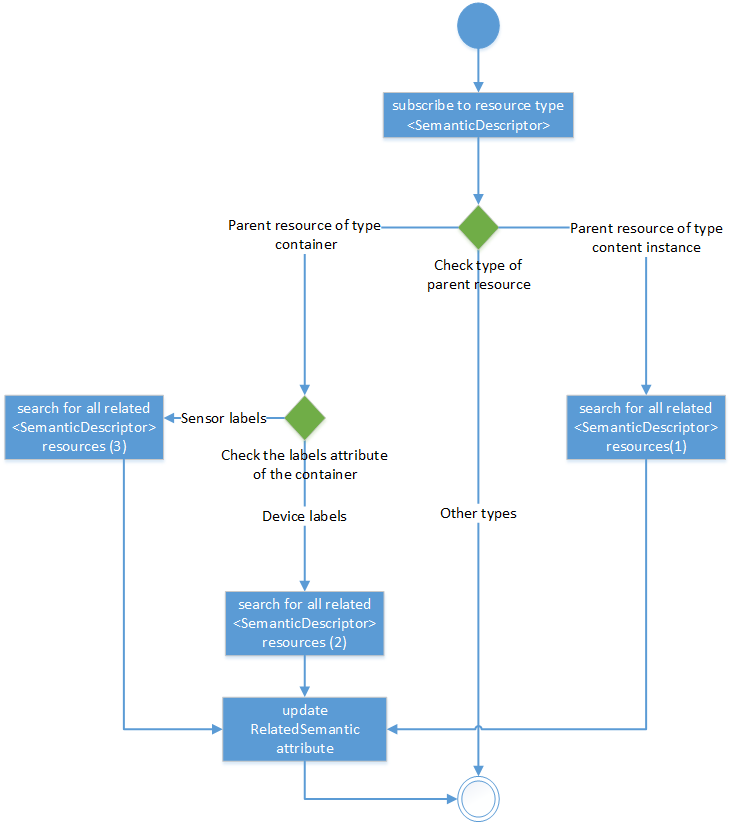
\includegraphics[width=1\textwidth]{resources/images/rsdiagram}
    \caption{Activity diagram of the \textit{RelatedSemantic} attribute update process. }\label{fig:contrib2:rs2}
\end{figure}

In the beginning, the Semantic filtering and discovery module subscribe to all available resources of type <semanticDescriptor> which are created by the Semantic Annotation module. Then, it starts checking the type of the parent resource of the candidate <semanticDescriptor> resource to figure whether it pertains to a resource of type container or of type content instance. In case the resource is of type content instance, the Semantic filtering and discovery module update the \textit{RelatedSemantic} attribute of the candidate resource with all the related <semanticDescriptor> resources. This is mainly done by adding the path of the <semanticDescriptor> resource presenting the sensor in which the candidate resource is made available and the path of the <semanticDescriptor> resource presenting the device of that particular sensor. Otherwise, in case the parent resource of the candidate <semanticDescriptor> resource is of type container, the Semantic filtering and discovery module shall retrieve the \textit{labels} attribute of its parent resource by extracting the parent resource itself. Then depending on the content of the labels attribute, the Semantic filtering and discovery module perform the update process of the \textit{RelatedSemantic} attribute. As illustrated in the figure there are mainly two situations. The first situation is when the content of the labels attribute conform to one of the sensors labels presented in the table. In this case, the Semantic filtering and discovery module update the \textit{RelatedSemantic} attribute with the path of the <semanticDescriptor> resource presenting the device of that particular sensor and with all paths of the <semanticDescriptor> resources that annotate its content Instances. Since that each container can have a limited number of instances which is defined in its MaxNumberOfInstance attribute, the Semantic filtering and discovery module shall limit the paths of the <semanticDescriptor> resources of the <contentInsctances> available in the \textit{RelatedSemantic} to the maximal number of instances available for each container. The second situation occurs when a device label is presented. In this case, the Semantic filtering and discovery module update the \textit{RelatedSemantic} attribute with the path of all the <semanticDescriptor> resources presenting all the sensors provided by the device and all their content instances. The number of paths of the <semanticDescriptor> resources of the <contentInsctances> exhibited in the \textit{RelatedSemantic} attribute should be limited to the number of instances of the device container as well.



\subsection{Design and Functions of the Semantic Repository }

The preceding section described the detailed architecture of the semantic annotator component responsible of semantically annotating the content of targeted resources. Thus, the relationship and value information modeled using different ontologies are stored with a resource in its <semanticDescriptor> resources. Due to the fact of the large heterogeneous data annotated and the limited lifetime of some resources, this approach is not completely efficient for Semantic Queries. In fact, Semantic Query is a necessary function in M2M system because it provides full support for resource reasoning, annotation and discovery. This is mainly done by using a Semantic Graph Storage for the Semantic Triples. \par 
Therefore, the semantic repository designed for this thesis and presented here provides means to store semantics annotation pertaining to all the annotated resources and full support for Semantic Queries. This repository contains mainly a set of triples extracted from all the <semanticDescriptor> resources stored depending on the ontology used for modeling the information within each resource. For example in case there are two different ontologies used to model the information and data, the semantic repository will create for each ontology a specific Semantic Graph Store. \par 
As outlined in the previous chapter, the Semantic Repository component is composed of two coupled modules. The detailed design and function of each module are presented herein.

\subsubsection{Repository module }
the semantic repository is responsible of gathering all the semantic information and data provided by the semantic annotator component to be stored.
In this context, the semantic repository subscribes to the resource of type <semanticDescriptor> using the internal subscription/notification mechanism previously presented in~\ref{sec:contrib2:Environment}. Thus, it grants access to all the attributes available and required for accomplishing the Graph Storage. When a new <semanticDescriptor> is available or when modifications to a resource are made, a notification sends by the subscription hosting CSE to the Semantic Repository. Furthermore, the notification scope includes tracking changes of attributes and child resources directly related to the <semanticDescriptor> resource. \par 
When receiving a notification from the hosting CSE about a newly created resource of type <semanticDescriptor>, the Semantic Repository shall go through the following actions in the aim of storing the information retrieved. Those actions are described in the figure~\ref{fig:contrib2:store}.

\begin{figure}[htbp]
    \centering
    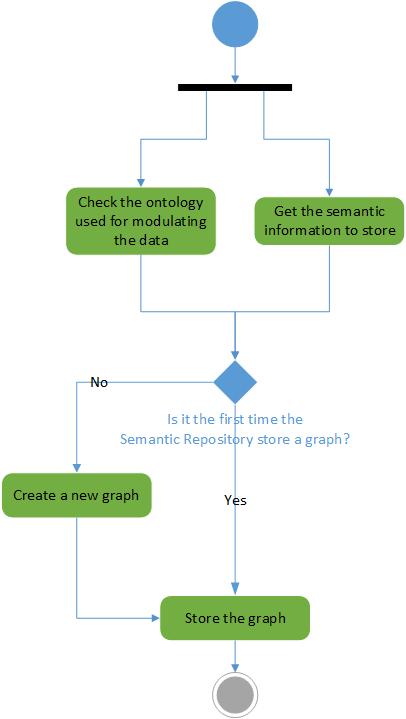
\includegraphics[width=.6\textwidth]{resources/images/storage}
    \caption{Activity diagram of the triplestore process. }\label{fig:contrib2:store}
\end{figure}
For each new resource of type <semanticDescriptor>, the Semantic Repository extract the semantic information from the descriptor attribute. In case the data and information are semantically described with more than one ontology, the Semantic Repository check the OntologyRef Attribute to figure the reference URL of the ontology used. Thus, if the ontology used for semantically describing information is not yet stored, the Semantic Repository create a new graph for that specific ontology. Finally the Semantic Repository store or concatenate the graph with the graph already stored. Concerning the Graph storage, there are two architectural approach considered within this work. For this reason, the design and functions of Semantic analysis and query module depends principally on the design of the graph storage. Thus, it is explained within each approach.

\paragraph{First approach }
After extracting the semantic information to be stored from all the <semanticDescriptor> resource available, the Semantic Repository deposes all information gathered, into a local, centralized Semantic Graph Store (i.e. Semantic Repository) as illustrated in the figure~\ref{fig:contrib2:1store}. In this manner, the Semantic repository is implemented as a linked-data database allowing the management of semantic operations.\par 
\begin{figure}[htbp]
    \centering
    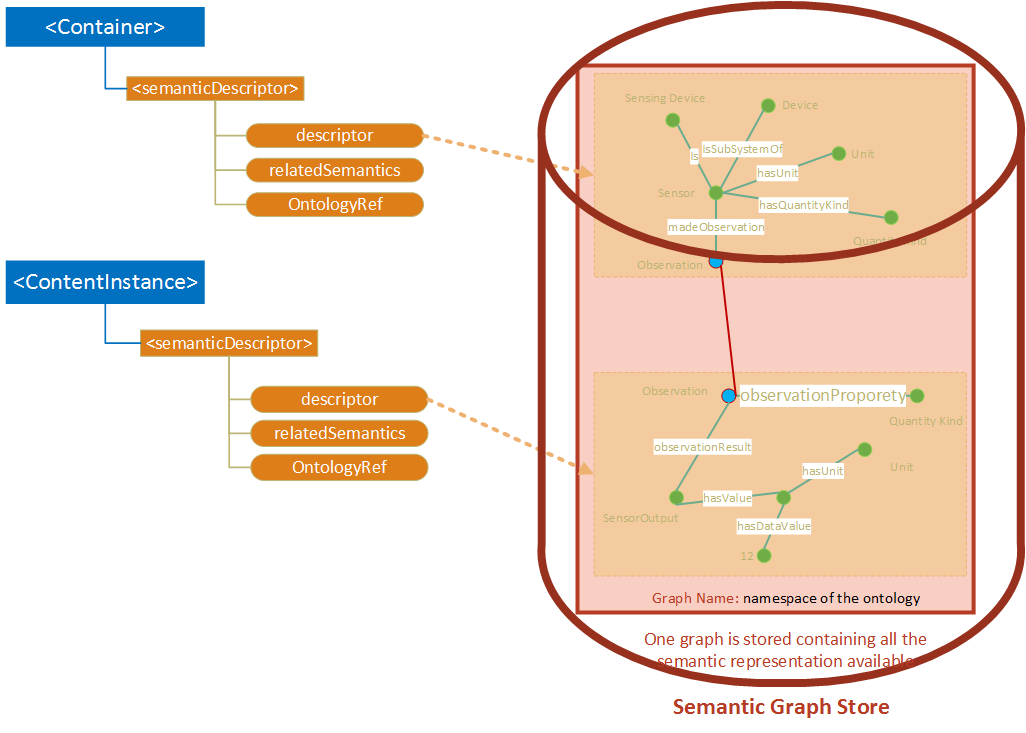
\includegraphics[width=.9\textwidth]{resources/images/1store}
    \caption{The triplestore process using the first approach. }\label{fig:contrib2:1store}
\end{figure}
This architectural solution provides full support for Semantic Queries with all Semantic Triples available in the Semantic Graph Store. Thus, the Semantic Repository handles the client’s queries (e.g. SPARQL queries) to find the resource semantics information available in the Semantic Graph Store by executing the query in the whole graph and return back the results. In case the resource information are modeled with more than one ontology, the Graph Store shall include for each ontology a single graph. Therefore, it is required to use a quadstore storage which provide the possibility to name each graph with the namespace of the ontology used to annotate the data.\par 
Within this approach, the Semantic analysis and query module is responsible mainly for providing means to perform Semantic Query on the distributed Semantic Descriptors. As illustrated in the sequence diagram in the figure there are several steps to follow for the purpose of performing Semantic Queries on the distributed Semantic Descriptors. It all start by an originator (typically a CSE or EA) sending a Semantic Query operation request in the form of SPARQL request with the option of specifying the resource, sensor, device or service to be discovered. For example an originator specifies the resource to be semantically queried or the device name. In case the originator does not specify a resource or any data to be semantically discovered and queried the Semantic analysis and query module conducts the semantic query with the Semantic Graph sored in the Semantic Repository and it composes a response to the originator containing the semantic queries results. Otherwise, if the originator specifies the resource to be Semantically Queried, the semantic analysis and query module shall conduct a semantic descriptor discovery among all the resource tree. Then it retrieve the resource discovered and extract all links presented in the <RelatedSemantics> attribute to create a local temporary graph constructed from the semantic descriptions retrieved from all related semantic descriptor resources. Finally, the Semantic analysis and query module conduct a semantic query in the temporary graph and compose a response with the Semantic Query results. 

  
\paragraph{Second approach }

In contrast to the first approach, within this approach each semantic description extracted from each descriptor attribute is stored in a single graph as showing in figure~\ref{fig:contrib2:2store}.
\begin{figure}[htbp]
    \centering
    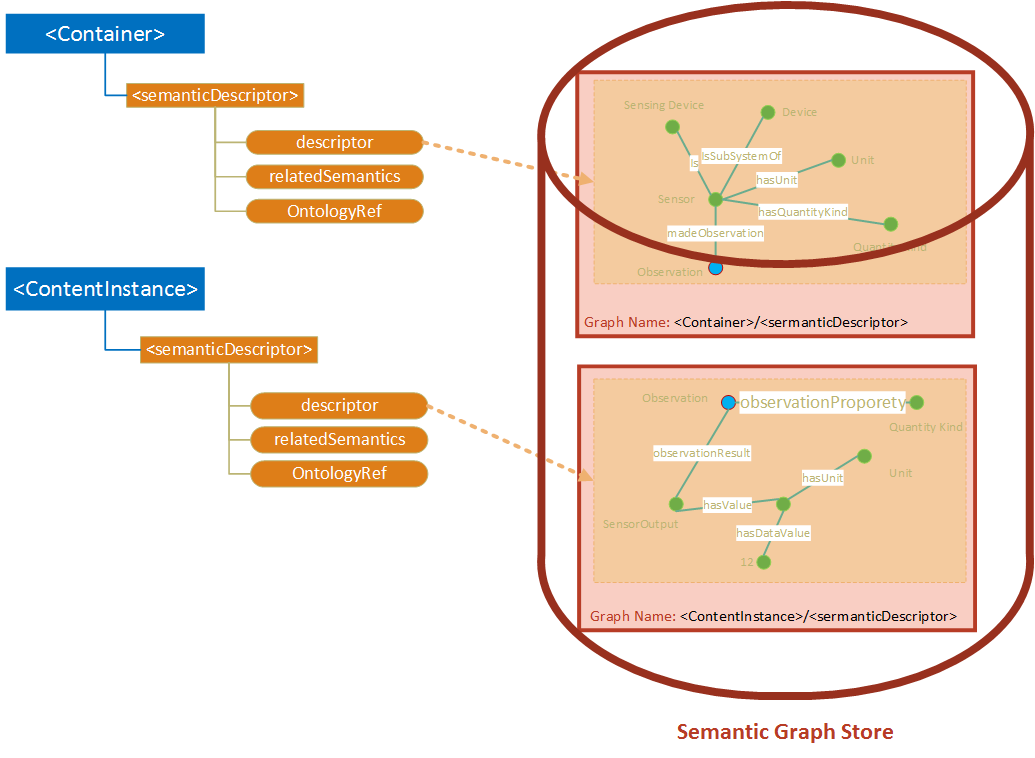
\includegraphics[width=.9\textwidth]{resources/images/2store}
    \caption{The triplestore process using the second approach. }\label{fig:contrib2:2store}
\end{figure}

Therefore, using this approach require the use of a quadstore to name each graph retrieved form the set of the available <semanticDescriptor> resources. The idea behind this approach is not only to optimize the query execution process, but also to provide means to perform Semantic Query on the discovered Semantic Descriptors presented in hierarchical Resource Tree without requiring the creation of a local temporary Semantic Graph Store to dispose all the Semantic Triples extracted. From this perspective, each graph is named with its <semanticDescriptor> resource URL. Thus, when performing a Semantic Query on the discovered Semantic Descriptors, it is possible for the Semantic analysis and query module to retrieve all the related semantic descriptors to the candidate resource from its \textit{RelatedSemantic} attribute and to compose a query targeting those specific resources. The figure illustrate the overall semantic query process between an originator and a receiver.

Although this approach provides a practical solution to perform Semantic Query with Distributed Semantic Descriptors without the need of a temporary graph store, the Semantic Query with all Semantic Triples Contained in the Graph Store might get complicated compared to the first approach. Since that each Semantic Triples extracted form each Semantic Descriptor resource is stored in a dedicated graph as showing in figure~\ref{fig:contrib2:2store}, the originator is required to specify all the Semantic Descriptors where the query shall be performed. Moreover, in our overall architecture, it is possible to semantically annotate data and information using two ontologies. For this reasons adapting this approach require the use of two dedicated Semantic graph store, one for each ontology used. Thus, it is more convenient to use for each ontology not only a dedicated Semantic Annotator component as it was explained in , but also a dedicated Semantic repository component.

\paragraph{Specific Design Decisions }
The main differences between the two approach is the handling of the Semantic Queries on the distributed Semantic Descriptors. The first approach consist of providing a centralized Graph store with the possibility to create a temporary graph to perform the Semantic Queries on the distributed Semantic Descriptors. In the other hand, the second approach consist of storing the semantic description of all resources in a distributed manner. Thus, it is possible to perform Semantic Queries on the distributed Semantic Descriptors without requiring the creation of a temporary semantic graph.\par 

Based on the understanding of the design architecture of each approach used to provide Semantic Queries on the distributed Semantic Descriptors, it is possible to conclude that both of them are relaying on the \textit{RelatedSemantic} attribute of the candidate resource. Therefore, the performance of each approach is directly related to the \textit{RelatedSemantic} attribute which signify that in case this attribute includes a huge set of links to be queried, it is more appropriate to adapt the second approach because it does not require the creation of a local temporary graph. In fact, as it was previously explained this approach conduct directly the Semantic Query on the centralized Graph Store in all cases including querying the distributed Semantic Descriptors . Otherwise, in case the \textit{RelatedSemantic} attribute includes a limited set of links to be queried which is the case of our work, it is more appropriate to adapt the first approach because it provide an easier and more efficient method to query the semantic information residing in the local Semantic Graph store. \par 

Since that the \textit{RelatedSemantic} attribute can have a limited set of links in the core design of the Semantic annotation Extension as it was explained in the previous section, the Repository module adapt the first approach to store and query the semantic information and data provided by the semantic annotator component.




%TR-0033-Study_on_Enhanced_Semantic_Enablement-V0_2_0

\section{Conculsion}
    \cleardoublepage
\chapter{Implementation}\label{sec:contrib3}\minitoc\vspace{.5cm}



\index{Contribution 3}

\section{Introduction}
As it was described in state of the art, the OpenMTC features are aligned with the oneM2M specification. Therefore it implements a CSE at the Front-end gateway and a second CSE at the back-end server. Moreover, it provides several methods to communicate with non-M2M enabled devices through dedicated Inter-working proxy Entities. \par 
Based on the design and specification described in Chapter~\ref{sec:contrib2}, this chapter describes the actual implementation of this specification in the form of a prototype solution as part of the OpenMTC platform.\par 
First, the implementation environment of the Semantic Annotation Extension and the overall structure is specified. Afterward, the implementation of the different components and modules are explained.

\section{Environment Specification}

The implementation environment can be described as follow: The OpenMTC platform is communicating with non-M2M enabled devices that provide sensed data thought its Interworking Proxy Entity. \par 
Within this work, the devices are using the ZigBee wireless language as a connectivity technology. In this context an overview of the hardware environment is given at first and then the software environment is described.
\subsection{Hardware environment}
The hardware environment is composed of three main components:
\begin{itemize}
\item \textbf{ZigBee wireless M-Bus Multi-Sensor 2}:
It is a multi-sensing device that uses ZigBee wireless language to provide full measures and monitors of various environmental factors such as temperature, motion, humidity, air pressure and brightness. It includes the following features:
\begin{itemize}
    \item Temperature (up to 0.3°C; resolution 0.1°C on demand).
    \item Motion Detection.
    \item Presence Detection.
    \item Relative humidity.
    \item Brightness (/FS only).
    \item Air pressure (/FS only).
    \item Uses ZigBee IEEE 802.15.4.
\end{itemize}
\item \textbf{Gateway}:
\item \textbf{A workstation computer}:
A workstation where OpenMTC is running.
\end{itemize}

\subsection{Software environment}

The Semantic Annotation Extension is completely implemented using Python 2.7 language. Therefore the integrated development environment (IDE) used within this work is JetBrains PyCharm professional edition version 2016.3.2 which is a cross-platform that works on Windows, OS X and Linux.\par 
In the following list a summery of the operating system, frameworks, software and the most relevant library used within this work:
\begin{itemize}
\item \textbf{Ubuntu 14.04.4 LTS}: This Linux distribution was used as an OpenMTC platform where the development of the Extension is done. For the implementation propose a 64 bit version of the distribution was used together with a kernel version 3.16.0-77-generic.

\item \textbf{OpenMTC and its ZigBee Interworking Proxy Entity (ZigBeeIPE)}: The ZigBeeIPE is used for the mapping of the different set of outputs provided by the ZigBee multi-sensor device. 
\item \textbf{Postman chrome App}: Postman is a Chrome browser App. This Chrome App is used within this work to construct CRUD requests on the oneM2M resources of the OpenMTC platform, save them for later use and analyze the responses sent by the OpenMTC gateway. Thus, through its simple user interface it provides means to test, verify and manipulate the resources available effortless. Postman includes different feature relevant to this work such as: 
\begin{itemize}
\item CRUD methods (Create, Retrieve Update and Delete).
\item Fast request creation.
\item History of the sent requests.
\item A good user interface (UI)
\end{itemize}
\item \textbf{RDFLib}: is a pure and extensive python package for working with RDF. It contains most things required to work with RDF such as parsers, serializers for RDF/XML, N3, Turtle and RDFa and a SPARQL 1.1 implementation. RDFLib version used within this thesis is rdflib-4.2.2.
\item \textbf{Open Link Virtuoso}: is a native triplestore that provide an RDF web application server and file server functionality for storing and querying RDF data. It provides mainly a mechanism for persistent storage and access of RDF graphs which is used within this work to store the different graphs extracted from the targeted resources.

\item \textbf{Flask}: is a web framework written in Python which does not require particular tools or libraries. This framework is used within this work to create a server from where OpenMTC applications can perform discovery requests based on semantic on a the IPE resources.
\end{itemize}
\section{Development Method}
In order to set a development strategy for the Semantic Annotation Extension implementation, the V-model illustrated in Figure~\ref{fig:contrib2:v}, is adapted as a reference development method design. It was chosen from the other development models because, in one hand the requirements of this work are well understood, in the other hand it fits well for single person development. Moreover, this model is simple, easy to use and it promotes proactive defect tracking by finding defects at early stages. \par 
\begin{figure}[htbp]
    \centering
    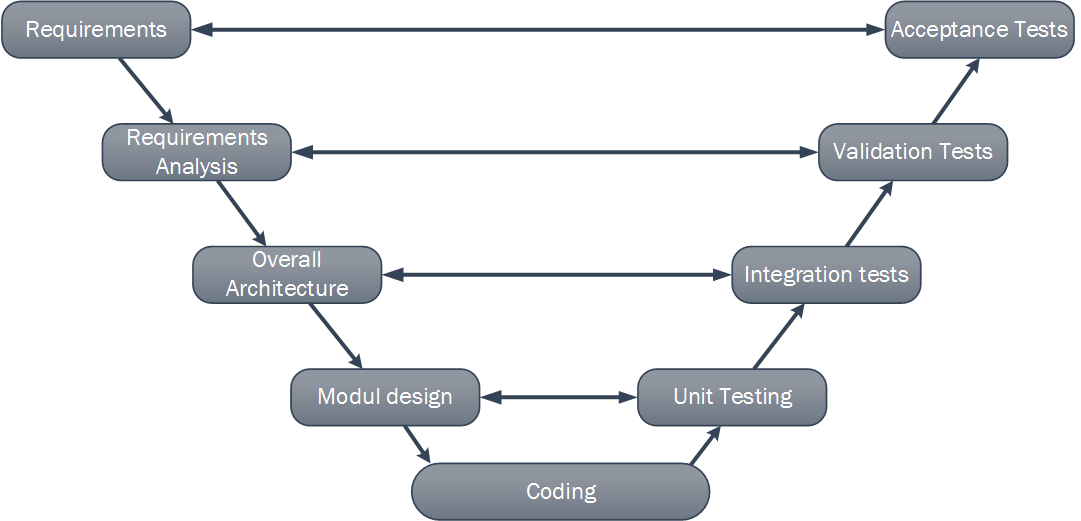
\includegraphics[width=1\textwidth]{resources/images/vmodel}
    \caption{V-model representation}\label{fig:contrib2:v}
\end{figure}
Since that the several steps of the V-model are sequentially passed through, each step should be completed before moving to the next one. Thus, the process starts by analyzing and collecting the requirements. Based on the collected requirements, the overall design system architecture is documented. Afterward, the implementation step starts by developing the core skeleton of the design previously documented and sequentially adding new functional units. Finally as illustrated in figure~\ref{fig:contrib2:v} there are several steps used to validate the process with various tests (e.g. Unit testing, component testing\ldots).

\section{Project Structure}

%But there are several programming language used for implementing the user interfaces within this work.

%As it was described in the chapter, the OpenMTC feature are aligned with the oneM2M specification. Therefore it implements a CSE at the Front-end gateway and a second CSE at the back-end server. Moreover it provides several method to communicate with non-M2M enabled devices through dedicated Inter-working proxy Entities. \par 

%This extension allows OpenMTC to create a pool of common data available in a specific environment and to share them between different OpenMTC applications, without requiring the information of the data type or content (units, meta data, context, etc.) in advance. Moreover, our implementation consist as well in enabling data access via SPARQL interface and oneM2M standard. \par 
%As outlined in the previous chapter, the goal of this thesis is to design and implement a semantic annotation extension for the OpenMTC Platform aiming to provide semantic interoperability for accessing resources and interpreting data from different stakeholders. \par 


%reference for the device and everything



\section{Conclusion}

\sidenote{Summary}
\todomid{write}

\sidenote{Takeaway 1}
\todomid{write}

\sidenote{Takeaway 2}
\todomid{write}

\sidenote{Takeaway 3}
\todomid{write}

\sidenote{Next chapter}
\todomid{write}

    \cleardoublepage
\chapter{Evaluation}\label{sec:eval}\minitoc\vspace{.5cm}
\index{Evaluation}\index{Validation}\index{Verification}

\section{Introduction}

\begin{wrapfigure}{r}{0.2\textwidth}
    \centering
    \includegraphics[width=0.2\textwidth]{resources/images/example3}
\end{wrapfigure}

\sidenote{Overview}
\todomid{write about \Cref{sec:eval:tec}}

\begin{figure}[htbp]
    \centering
    \includegraphics[width=.8\textwidth]{resources/images/example3}
    \caption{Choice of verification and validation techniques~\cite{li2002design}}\label{sec:eval:tec}
\end{figure}

\sidenote{Approaches}
\todomid{write}

\sidenote{Structure of Research}
\todomid{write about \Cref{fig:hourglass:evaluation}}

\begin{figure}[htpb]
    \centering
    \includegraphics[width=.55\textwidth]{resources/images/example3}
    \caption{Placement of the evaluation in the structure of research}\label{fig:hourglass:evaluation}
\end{figure}

\section{Experimental Validation}

\sidenote{Overview}
\todomid{write about \Cref{tbl:eval:experiments}}

\begin{sidewaystable}
      \centering
      \captionsetup{type=table}
      \caption{Sideways table}
      \begin{tabular}{lllllll}\toprule
  \textbf{Experiment 1}   & \textbf{Experiment 2}  & \textbf{Experiment 3} & \textbf{Experiment 4} & \textbf{Experiment 5} & \textbf{Experiment 6} & \textbf{Experiment 7}  \\ \midrule
  CATCH & ME & IF & YOU & CAN & \emph{NOW} & OR NEVER \\
  CATCH & ME & IF & YOU & CAN & \emph{NOW} & OR NEVER \\
  CATCH & ME & IF & YOU & CAN & \emph{NOW} & OR NEVER \\
  CATCH & ME & IF & YOU & CAN & \emph{NOW} & OR NEVER \\
  CATCH & ME & IF & YOU & CAN & \emph{NOW} & OR NEVER \\
  CATCH & ME & IF & YOU & CAN & \emph{NOW} & OR NEVER \\
  CATCH & ME & IF & YOU & CAN & \emph{NOW} & OR NEVER \\
  CATCH & ME & IF & YOU & CAN & \emph{NOW} & OR NEVER \\
  CATCH & ME & IF & YOU & CAN & \emph{NOW} & OR NEVER \\
  CATCH & ME & IF & YOU & CAN & \emph{NOW} & OR NEVER \\
  CATCH & ME & IF & YOU & CAN & \emph{NOW} & OR NEVER \\
  \bottomrule
      \end{tabular}\label{tbl:eval:experiments}
\end{sidewaystable}


\subsection{Setup 1}

\sidenote{Overview}
\todomid{write}

\sidenote{Integration}
\todomid{write about \Cref{eq:var_idb}}

\small
\begin{equation}
  \begin{array}{l}
    \displaystyle t^{p_d}_{fw}(d) = \max_{d}(t_{child_{i}}) \\
    \displaystyle t^{p_d}_{db}(d) = \sum_{i=1}^{d} t_{db_{i}} \\
    \displaystyle t^{p_d}_{pc}(n,d) =
    	\begin{cases}
        	t_{pc}(d) + c(n) & \text{if $d = 1$,}\\
        	t_{pc}(d) + c(n) + \max(t_{avail}(d)) & \text{if $d>1$.}\\
        \end{cases}
  \end{array}\label{eq:var_idb}
\end{equation}
\normalsize

\sidenote{Example}
\todomid{write about \Cref{lst:eval:exp1}}

\needspace{5\baselineskip}\lstset{caption=Experiment 1, label=lst:eval:exp1,
language=ttl, breaklines=true, numbers=left,
stepnumber=1, frame=single, inputencoding=utf8/latin1}~\lstinputlisting{resources/code/example.java}

\subsection{Setup 2}

\sidenote{Overview}
\todomid{write}

\sidenote{Integration}
\todomid{write}

\sidenote{Example}
\todomid{write about \Cref{fig:eval:sub1,fig:eval:sub2,fig:eval:sub}}

\begin{figure}
    \begin{subfigure}[b]{.455\textwidth}
      \centering
      \includegraphics[width=.9\textwidth,frame]{resources/images/example3}
      \caption{Subfig 1}\label{fig:eval:sub1}
    \end{subfigure}~\begin{subfigure}[b]{.545\textwidth}
      \centering
      \includegraphics[width=1\textwidth,frame]{resources/images/example3}
      \caption{Subfig 2}\label{fig:eval:sub2}
    \end{subfigure}
    \caption{Sub Figures}\label{fig:eval:sub}
\end{figure}


\section{Performance Evaluation}

\sidenote{Overview}
\todomid{write}

\subsection{Evaluation 1}

\sidenote{Setup}
\todomid{write}

\sidenote{Cost Metrics}
\todomid{write}

\sidenote{Optimizing}
\todomid{write}

\sidenote{Performance Comparison}
\todomid{write}

\subsection{Evaluation 2}

\sidenote{Setup}
\todomid{write}

\sidenote{Response Times}
\todomid{write}
\begin{itemize}[noitemsep]
  \item \emph{In}: 159 ms $\pm$ 21 ms (95\% CI)
  \item \emph{Out}: 33 ms $\pm$ 5 ms (95\% CI)
  \item \emph{Between}: 238 ms $\pm$ 9 ms (95\% CI)
  \item \emph{After}: 45 ms $\pm$ 1 ms (95\% CI)
  \item \emph{Under}: 215 ms $\pm$ 2 ms (95\% CI)
  \item \emph{Over}: 148 ms $\pm$ 3 ms (95\% CI)
\end{itemize}

\sidenote{Scalability}
\todomid{write}

\section{Observational Validation}

\sidenote{Overview}
\todomid{write}

\subsection{Project 1}

\sidenote{Overview}
\todomid{write}

\sidenote{System Specification}
\todomid{write}

\sidenote{Extraction}
\todomid{write}

\sidenote{Example}
\todomid{write}

\subsection{Project 2}

\sidenote{Overview}
\todomid{write}

\sidenote{System Specification}
\todomid{write about \Cref{fig:eval:side}}

\begin{figure}[htbp]
    \centering
    \includegraphics[height=.5\textwidth,angle=270]{resources/images/example3}
    \caption{Sideways figure}\label{fig:eval:side}
\end{figure}

\sidenote{Extraction}
\todomid{write}

\sidenote{Example}
\todomid{write}

\section{Deployments}

\sidenote{Overview}
\todomid{write}

\subsection{Installation 1}

\sidenote{Overview}
\todomid{write}

\sidenote{Integration}
\todomid{write}


\subsection{Installation 2}

\sidenote{Overview}
\todomid{write}

\sidenote{Integration}
\todomid{write}

\section{Code Verification}

\sidenote{Overview}
\todomid{write}

\sidenote{Static Tests}
\todomid{write}

\sidenote{Continuous Integration}
\todomid{write}

\sidenote{Test Coverage}
\todomid{write}

\section{Comparative Analysis}

\sidenote{Overview}
\todomid{write}

\subsection{Requirement Evaluation}

\sidenote{\Cref{tbl:reqs:compare}}
\todomid{write}

\begin{tabularx}{\textwidth}{p{2cm}X}
    \caption{Mapping requirements against own approach}\label{tbl:reqs:compare}\\
    \toprule
    \textbf{Requirements}& \textbf{Approach}  \\\midrule
    \endfirsthead%
    \toprule
    \textbf{Requirements}& \textbf{Approach}  \\\midrule
    \endhead%
\ref{req:stakeholder1:foo}\newline(Foo) &
\todomid{write}
\\\midrule

\ref{req:stakeholder1:bar}\newline(Bar) &
\todomid{write}
\\\midrule

\ref{req:stakeholder2:foo}\newline(Foo) &
\todomid{write}
\\\midrule

\ref{req:stakeholder2:bar}\newline(Bar) &
\todomid{write}
\\\midrule

\ref{req:stakeholder3:foo}\newline(Foo) &
\todomid{write}
\\\midrule

\ref{req:stakeholder3:bar}\newline(Bar) &
\todomid{write}

\\\bottomrule
\end{tabularx}

\subsection{Comparison with Other Approaches}

\sidenote{Overview}
\todomid{write}

\sidenote{\Cref{tbl:approaches:compare}}
\todomid{write about \Cref{tbl:approaches:compare}}

\begin{tabularx}{\textwidth}{p{2cm}LLLLLL}
    \caption{Comparison of related work with own approach}\label{tbl:approaches:compare}\\
    \toprule
    \textbf{Requirements} & \textbf{Related 1} & \textbf{Related 2} & \textbf{Related 3} & \textbf{Related 4} & \textbf{Related 5} & \textbf{Own Approach} \\\midrule
    \endfirsthead%
    \toprule
    \textbf{Requirements} & \textbf{Related 1} & \textbf{Related 2} & \textbf{Related 3} & \textbf{Related 4} & \textbf{Related 5} & \textbf{Own Approach} \\\midrule
    \endhead%

\ref{req:stakeholder1:foo}~\ref{req:stakeholder1:bar} & \textbf{(+)} & \textbf{(++)} & \textbf{(o)} & \textbf{(-)} & \textbf{(o)} & \textbf{(+++)} \\
(\ac{ABAC}) & \ac{ABAC} \ac{ABAC} v3, \ac{ABAC} \ac{ABAC} & \ac{ABAC} \ac{ABAC} v2, \ac{ABAC}, native \ac{ABAC} & \ac{ABAC} & native \ac{ABAC} & \ac{ABAC} \ac{ABAC} v2 & \ac{ABAC} \ac{ABAC} v3, \ac{ABAC} \ac{ABAC}, \ac{ABAC}, native \ac{ABAC}, native \\\midrule

\ref{req:stakeholder3:foo} & \textbf{(o)} & \textbf{(++)} &  & & \textbf{(++)} & \textbf{(+)} \\
(Details) & via foo & by bar / role-foo & --- & --- & bar / foo & foo-bar \\\midrule

\ref{req:stakeholder2:foo}~\ref{req:stakeholder2:bar}~\ref{req:stakeholder3:bar} & \textbf{(+)} & \textbf{(+)} & & \textbf{(+)} & \textbf{(+)} & \textbf{(+)} \\
(Barli) & via barli & via fooli & --- & via bar-foo & via foo-bar & via bar-bar \\\bottomrule
\end{tabularx}

\section{Conclusion}

\sidenote{Summary}
\todomid{write}

\sidenote{Takeaway 1}
\todomid{write}

\sidenote{Takeaway 2}
\todomid{write}

\sidenote{Takeaway 3}
\todomid{write}

\sidenote{Next chapter}
\todomid{write}

    \cleardoublepage
\chapter{Summary and Further Work}\minitoc\label{sec:summary}\vspace{.5cm}

\section{Overview}

\begin{wrapfigure}{r}{0.2\textwidth}
    \centering
    \includegraphics[width=0.2\textwidth]{resources/images/example3}
\end{wrapfigure}

\sidenote{Contributions}
\todomid{write}

\begin{figure}
    \centering
    \includegraphics[width=.55\textwidth]{resources/images/example3}
    \caption{Placement of the outlook in the structure of research}\label{fig:hourglass:outlook}
\end{figure}

\sidenote{Dissemination}
\todomid{write about \Cref{fig:hourglass:outlook}}

\section{Conclusions and Impact}

\sidenote{Context}
\todomid{write}

\sidenote{Contribution 1}
\todomid{write}

\sidenote{Contribution 2}
\todomid{write}

\sidenote{Contribution 3}
\todomid{write}

\section{Outlook}

\sidenote{Intro}
\todomid{write}

\sidenote{Application Area 1}
\todomid{write about \Cref{fig:outlook:aa1}}

\begin{figure}
    \centering
    \includegraphics[width=.85\textwidth]{resources/images/example3}
    \caption{Area 1~\cite{li2002design}}\label{fig:outlook:aa1}
\end{figure}

\sidenote{Application Area 2}
\todomid{write}

\sidenote{Application Area 3}
\todomid{write}

\sidenote{Application Area 4}
\todomid{write}

    \nolinenumbers
    \cleardoublepage

    \appendix
    \pagenumbering{Roman}
    \setcounter{page}{1}
    \cleardoublepage\chapter{Specifications}\minitoc\vspace{.5cm}

\section{Specification 1}\index{Specification 1}

\todomid{write about \Cref{lst:spec1}}

\lstset{language=ttl, breaklines=true, caption=Specification 1, %
emptylines=0,
label=lst:spec1, numbers=left, stepnumber=1, inputencoding=utf8}
\lstinputlisting{resources/code/example.java}


\section{Specification 2}\index{Specification 2}

\todomid{write about \Cref{lst:spec2}}

\lstset{language=ttl, breaklines=true, caption=Specification 2, %
emptylines=0,
label=lst:spec2, numbers=left, stepnumber=1, inputencoding=utf8}
\lstinputlisting{resources/code/example.java}


\cleardoublepage\chapter{Test Results}\minitoc\vspace{.5cm}

\section{Conformance Results}

\sidenote{Overview}
\todomid{write about \Cref{fig:test:result1,fig:test:result2}}

\begin{figure}[H]
    \centering
    \includegraphics[width=.9\textwidth,frame,page=1]{resources/images/example3}
    \caption{Test results (page 1)}\label{fig:test:result1}
\end{figure}

\begin{figure}[H]
    \centering
    \includegraphics[width=.9\textwidth,frame,page=1]{resources/images/example3}
    \caption{Test results (page 2)}\label{fig:test:result2}
\end{figure}

\section{Performance Results}

\subsection{Histograms}

\sidenote{Overview}
\todomid{write about \Cref{fig:eval:perf:hist:forms}}

\begin{figure}[H]
    \begin{subfigure}[b]{.5\textwidth}
      \centering
      \includegraphics[width=.95\textwidth,frame]{resources/images/example3}
      \caption{Form A}
    \end{subfigure}~\begin{subfigure}[b]{.5\textwidth}
      \centering
      \includegraphics[width=.95\textwidth,frame]{resources/images/example3}
      \caption{Form B}
    \end{subfigure}
    \caption{Histogram of Forms}\label{fig:eval:perf:hist:forms}
\end{figure}


\subsection{Lineplots}

\sidenote{Overview}
\todomid{write about \Cref{fig:eval:perf:line:lines}}

\begin{figure}[H]
    \begin{subfigure}[b]{.5\textwidth}
      \centering
      \includegraphics[width=.95\textwidth,frame]{resources/images/example3}
      \caption{Lines A}
    \end{subfigure}~\begin{subfigure}[b]{.5\textwidth}
      \centering
      \includegraphics[width=.95\textwidth,frame]{resources/images/example3}
      \caption{Lines A}
    \end{subfigure}
    \caption{Lineplot of the lines}\label{fig:eval:perf:line:lines}
\end{figure}


    \cleardoublepage
    \cleardoublepage
\chapter*{Acronyms}
\mtcaddchapter\addstarredchapter{Acronyms}
\markboth{Acronyms}{Acronyms}
\stepcounter{chapter}
\renewcommand*{\chapterthumbformat}{Acronyms}
\printacronyms[name={}, exclude-classes=exclude]

\cleardoublepage
\stepcounter{chapter}
\renewcommand{\glossaryname}{Glossary}
\markboth{\glossaryname}{\glossaryname}
\renewcommand*{\chapterthumbformat}{\glossaryname}
\printglossary%

\cleardoublepage
\chapter*{Bibliography}
\mtcaddchapter\addstarredchapter{Bibliography}
\markboth{Bibliography}{Bibliography}
\stepcounter{chapter}
\renewcommand*{\chapterthumbformat}{Bibliography}
\minitoc\vspace{.5cm}

\section*{List of Author's Publications Covered in this Thesis}
\nocite{li2002design}
\newrefcontext[labelprefix=a]
\printbibliography[keyword=own,heading=empty,category=cited]


\section*{References to Scientific Publications}
\defbibfilter{papers}{
  type=article
  or type=inproceedings
  or type=proceedings
  or type=journal
  or type=phdthesis
  or type=incollection
  or type=book
  or keyword=thesis
  and not keyword=W3C
  and not keyword=RFC
  and not keyword=ITU
  and not keyword=IEEE
  and not keyword=ANSI
  and not keyword=OGF
  and not keyword=web
  and not keyword=presentation
  and not keyword=workingpaper
}
\newrefcontext[labelprefix=p]
\printbibliography[filter=papers,heading=empty,category=cited,notkeyword=own]


\section*{Technical References}

\defbibfilter{standards}{
  keyword=W3C
  or keyword=RFC
  or keyword=TMF
  or keyword=ITU
  or keyword=IEEE
  or keyword=ANSI
  or keyword=OGF
  or keyword=ETSI
  or keyword=OneM2M
  or keyword=IETF
  or keyword=OMA
  or keyword=TMG
  or keyword=NIST
  or keyword=SNIA
  or keyword=OMG
  or keyword=DMTF
  or keyword=OASIS
  or type=techreport
  or keyword=deliverable
  or keyword=techreport
  or keyword=whitepaper
  and not keyword=web
  and not keyword=presentation
  and not keyword=workingpaper
}
\newrefcontext[labelprefix=t]
\printbibliography[filter=standards,heading=empty,category=cited,notkeyword=own]


\section*{Miscellaneous References}
\defbibfilter{misc}{
  keyword=web
  or keyword=presentation
  or keyword=workingpaper
}
\newrefcontext[labelprefix=m]
\printbibliography[filter=misc,heading=empty,category=cited,notkeyword=own]


\section*{Not referenced (will be empty)}
\todo{this section should be empty at the end}
\nocite{*}
\newrefcontext[labelprefix=x]
\printbibliography[heading=empty,notcategory=cited,notkeyword=own]


    \backmatter
    \cleardoublepage\cleardoublepage
\phantomsection
\stepcounter{chapter}
\renewcommand{\indexname}{Index}
\renewcommand*{\chapterthumbformat}{\indexname}
\markboth{\indexname}{\indexname}
\printindex%

\end{document}
% ------------------------------------------------------------------------------
